\chapter{Δομή και εξέλιξη αστέρων}
\label{ch:Chapter5}
{\hypersetup{linkcolor=black, pdfborder=0 0 1}
	\minitoc
	%\newpage
}

Όλες οι παρατηρούμενες ιδιότητες που έχουμε αναφέρει μέχρι στιγμής, είναι ιδιότητες της επιφάνειας του αστέρα. Γι' αυτό χρειαζόμαστε μια θεωρία αστρικής δομής για να εξάγουμε συμπεράσματα για τις ``εσωτερικές'' ιδιότητες των άστρων. Παρόλα αυτά, υπάρχουν μερικά παράθυρα για την άμεση παρατήρηση του τι συμβαίνει στο εσωτερικό, όπως παρατηρήσεις νετρίνων (μέχρι στιγμής αυτό ισχύει μόνο για τον Ήλιο) και ταλαντώσεις που μας δίνουν πληροφορίες για την ταχύτητα που ταξιδεύουν τα ηχητικά κύματα στο εσωτερικό και άρα για την πυκνότητα και θερμοκρασία που επικρατούν.
%% ---------------------------------------------------------------------------------------------------- %%
%% ---------------------------------------------------------------------------------------------------- %%
%% ---------------------------------------------------------------------------------------------------- %%
\section{Εσωτερική δομή αστέρων}
Το πρότυπο αστρικής δομής που είναι σήμερα αποδεκτό προτείνει ότι η ενέργεια που ακτινοβολούν οι αστέρες εκλύεται στον πυρήνα τους από θερμοπυρηνικές αντδράσεις σύντηξης. Η ενέργεια αυτή διαδίδεται προς την επιφάνεια του αστέρα είτε με τη μορφή ακτινοβολίας είτε με ρεύματα μεταφοράς ύλης, και τελικα ακτινοβολείται από την επιφάνειά του προς το διάστημα. Για να γνωρίσουμε το εσωτερικό του Ήλιου (και άλλων αστέρων) βασιζόμαστε σε θεωρητικά επιχειρήματα, από τα οποία οδηγούμαστε τελικά σε ένα σύστημα διαφορικών εξισώσεων. Το σύστημα αυτό αποτελείται, στην απλούστερη μορφή του, από τέσσερις διαφορικές εξισώσεις και στη μορφή αυτή περιγράφει το θεωρητικό πρότυπο ενός σφαιρικά συμμετρικού, στατικού και μη-περιστρεφόμενου αστέρα, το υλικό του οποίου βρίσκεται σε υδροστατική και τοπική θερμοδυναμική ισορροπία.
%% ---------------------------------------------------------------------------------------------------- %%
%% ---------------------------------------------------------------------------------------------------- %%
%% ---------------------------------------------------------------------------------------------------- %%
\subsection{Μηχανική ισορροπία}
Η υπόθεση της σφαιρικής συμμετρίας έχει ως συνέπεια ότι όλες οι εξαρτημένες μεταβλητές του προβλήματος (πίεση $P$, πυκνότητα $\rho$, θερμοκρασία $T$ κτλ) είναι συνάρτηση μόνο της ακτινικής απόστασης, $r$, από το κέντρο του αστέρα, $r \in [0, \dots, R]$. Σε ένα αστέρι που εξελλίσεται όπως θα δούμε με τον χρόνο, όλες οι ποσότητες εξαρτώνται από τον χρόνο αλλά αυτό δεν θα είναι προφανές από τον τρόπο που θα παρουσιάσουμε τις εξισώσεις: μία παράγωγος $d/dr$ (ή $d/dm$) θα πρέπει να εκλαμβάνεται ως μερική παράγωγος ως προς τη χωρική συντεταγμένη υπό σταθερό χρόνο.
%% ---------------------------------------------------------------------------------------------------- %%
%% ---------------------------------------------------------------------------------------------------- %%
%% ---------------------------------------------------------------------------------------------------- %%
\subsubsection{Εξίσωση συνέχειας μάζας}
Έστω σφαιρικός φλοιός πάχους $dr$ σε απόσταση $r$ από το κέντρο του αστέρα (σχήμα \ref{fig:spherical_shell_hydrostatic_equilibrium}). Η αρχή της διατήρησης μάζας μας δίνει για τη στοιχειώδη μάζα, $dm$:
$$dm = \rho(r) dV$$
Ο όγκος του φλοιού θα είναι ουσιαστικά η επιφάνεια της εσωτερικής σφαίρας επί το στοιχειώδες πάχος. Αυτό αποδεικνύεται εύκολα ως εξής
$$dV = \frac{4}{3} \pi (r+dr)^3 - \frac{4}{3} \pi r^3 = \frac{4}{3} \pi \left[ (r+dr)^3 - r^3 \right] \simeq 4\pi r^2 dr$$ καθώς ο τετραγωνικός και κυβικός όρος του $dr$ στο ανάπτυγμα του πολυωνύμου μπορούν να θεωρηθούν ότι είναι περίπου μηδέν όταν $dr \ll r$. Αυτό μας οδηγεί στην πρώτη διαφορική εξίσωση που περιγράφει την δομή ενός αστέρα, την \textbf{εξίσωση συνέχειας μάζας}

\begin{equation}
    \label{eq:mass_continuity_diff}
    \boxed{\frac{dm}{dr} = 4 \pi r^2 \rho(r)} 
\end{equation}
Η εξίσωση αυτή περιγράφει το πως κατανέμεται η μάζα, και πως η κατανομή αυτή δεν έχει ασυνέχειες (δεν υπάρχουν τρύπες).


\begin{figure}
    \centering
    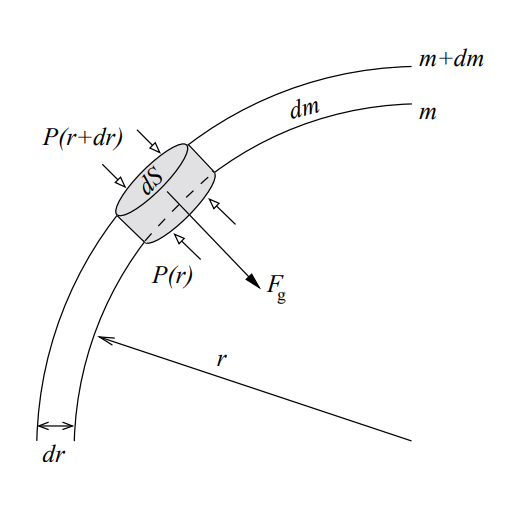
\includegraphics[scale=0.4]{Figures/spherical_shell_mechanical_equilibrium.png}
    \caption{Φλοιός σε ακτίνα $r$ και πάχος $dr$, μέσα σε σφαιρικά συμμετρικό αστέρι. Η μάζα του φλοιού είναι $dm = 4\pi r^2 \rho dr$. Στο σχήμα φαίνεται επίσης η πίεση και η βαρυτική δύναμη που ενεργούν σε ένα στοιχειώδες κυλινδρικό στοιχείο μάζας.}
    \label{fig:spherical_shell_hydrostatic_equilibrium}
\end{figure}

Η ολοκλήρωση της σχέσης \eqref{eq:mass_continuity_diff} μας δίνει την μάζα, $m(r)$, που περικλείει ένας σφαιρικός φλοιός ακτίνας $r$
\begin{equation}
        \label{eq:mass_coordinate}
    m(r) = \int_{0}^{R} 4\pi r^2 \rho(r) \,dr \hspace{0.5cm} (m \in 0,\dots,M)
\end{equation}

Επειδή η μάζα $m(r)$ αυξάνεται μονοτονικά προς την επιφάνεια του αστέρα, μπορούμε να χρησιμοποιήσουμε αυτή ως ακτινική συντεταγμένη αντί του $r$ (δηλαδή να χρησιμοποιήσουμε μια Λαγκραντζιανή περιγραφή αντί της μεθόδου του Euler). Έτσι η εξίσωση \eqref{eq:mass_coordinate} περιγράφει τη \textit{συντεταγμένη μάζας} (mass coordinate), η οποία είναι γενικευμένη συντεταγμένη (Lagrange coordinates) και κινείται μαζί με ένα στοιχειώδες κομμάτι του ρευστού. Αυτή η περιγραφή είναι προτιμότερη πολλές φορές καθώς η ακτίνα του αστέρα είναι συνάρτηση του χρόνου και μεταβάλλεται πολλές τάξεις μεγέθους κατά τη διάρκεια της εξέλιξής του.
Αντίθετα, η μάζα του μπορεί να θεωρηθεί σταθερή σε πρώτη φάση, γεγονός που απλοποιεί μερικές από τις χρονικές παραγώγους στις διαφορικές εξισώσεις που περιγράφουν την χημική σύσταση του αστέρα όπως θα δούμε. Έτσι, μπορούμε να γράψουμε όλες τις ποσότητες ως συνάρτηση της μάζας αντί του $r$ ως $r = r(m), \rho = \rho(m), P = P(m)$ κτλ. Κάνοντας τον μετασχηματισμό $r \rightarrow m$, η εξίσωση \eqref{eq:mass_continuity_diff} γράφεται ξανά:
\begin{equation}
    \label{eq:mass_continuity_diff_dm}
    \frac{d}{dm} = \frac{d}{dr} \cdot \frac{dr}{dm}  \longrightarrow \boxed{\frac{dr}{dm} = \frac{1}{4\pi r^2 \rho (r)}}
\end{equation}
%% ---------------------------------------------------------------------------------------------------- %%
%% ---------------------------------------------------------------------------------------------------- %%
%% ---------------------------------------------------------------------------------------------------- %%
\subsubsection{Το βαρυτικό πεδίο}
Τα αστέρια είναι αέρια σώματα που υποστηρίζονται από την ίδια τους την βαρύτητα (self-gravitating bodies), πράγμα που σημαίνει ότι η βαρύτητα παίζει καταλυτικό ρόλο στην εξέλιξή τους. Στη γενική, μη-σφαιρική περίπτωση, η βαρυτική επιτάχυνση είναι η κλίση (gradient) του βαρυτικού δυναμικού $\Phi$
$$\boldsymbol{g} = - \nabla \Phi$$
όπου το $\Phi$ είναι λύση της εξίσωσης Poisson 
\begin{equation}
    \label{eq:poisson_equation}
    \nabla^2 \Phi = 
    \begin{cases}
        0 & \text{για r > R}\\
        4\pi G \rho & \text{για r < R}
    \end{cases}
\end{equation}

Για μία σφαιρική κατανομή μάζας $M$, μπορούμε να θεωρήσουμε ότι όλη η μάζα είναι συγκεντρωμένη σε ένα σημείο στο κέντρο. Τότε, το βαρυτικό δυναμικό $\Phi$ σε απόσταση $r>R$ από το κέντρο, ισούται με το έργο ανά μονάδα μάζας που απαιτείται για να φέρουμε ένα σώμα μάζας $m$ από το άπειρο, σε αυτό το σημείο
\begin{equation}
    \Phi = \frac{1}{m}\int_{\infty}^{r} \boldsymbol{F_{\text{gr}}} \cdot d\boldsymbol{r} = \frac{1}{m} \int_{\infty}^{r} G\frac{M \,m }{r^2} \,dr \Rightarrow \Phi = - \frac{G \,M}{r}
\end{equation}
H βαρυτική επιτάχυνση γράφεται απλά $g = d\Phi / dr$ και σε ακτίνα $r$ (ή ισοδύναμα σε συντεταγμένη μάζας $m$) δίνεται από 
\begin{equation}
    \label{eq:gravitational_field}
    g = G \frac{m}{r^2}
\end{equation}
Σφαιρικοί φλοιοί που βρίσκονται σε ακτίνα μεγαλύτερη από $r$ δεν εφαρμόζουν κάποια δύναμη, άρα το $g$ εξαρτάται μόνο από την κατανομή της μάζας μέσα στον φλοιό ακτίνας $r$ (shell theorem). Το συμπέρασμα αυτό μπορεί να αποδειχθεί με τη βοήθεια του νόμου του Gauss από τον διανυσματικό λογισμό σύμφωνα με τον οποίο "το επιεπιφάνειο ολοκλήρωμα μια διανυσματικής συνάρτησης σε μια κλειστή επιφάνεια S ισούται με το τριπλό ολοκλήρωμα της απόκλισης (divergence) της διανυσματικής αυτής συνάρτησης στον όγκο V που περικλείεται από την κλειστή επιφάνεια"
\begin{equation}
    \label{eq:gauss_law_vector_calculus}
    \oiint_S \boldsymbol{f} \cdot d \boldsymbol{S} = \iiint_V (\nabla \cdot \boldsymbol{f}) \,dV 
\end{equation}
Θέτωντας $\boldsymbol{f} = \boldsymbol{g}$, προκύπτει ότι το αριστερό μέλος της σχέσης \eqref{eq:gauss_law_vector_calculus} γράφεται
\begin{equation}
    \label{eq:left_hand_side_gauss_law}
    \oiint_S \boldsymbol{g} \cdot d \boldsymbol{S} = \oiint_S (\boldsymbol{g} \cdot \hat{\eta}) \, dS = - 4\pi r^2 g
\end{equation}
Το παραπάνω αποτέλεσμα προκύπτει από τη σφαιρική συμμετρία του βαρυτικού πεδίου του αστέρα. Λόγω της συμμετρίας αυτής το πεδίο έχει μόνο ακτινική συνιστώσα, η οποία μάλιστα έχει σταθερή τιμή πάνω στη σφαιρική επιφάνεια S. Άρα, με την ένταση του βαρυτικού πεδίου να βγαίνει εκτός ολοκληρώματος, το κλειστό επικαμπύλιο ολοκλήρωμα ισούται με την επιφάνεια της σφαίρας με ακτίνα $r$. Το μείον προκύπτει επειδή το $\boldsymbol{g}$ με το διάνυσμα επιφάνειας $d\boldsymbol{S} = dS \cdot \hat{\eta}$ είναι συγγραμικά αλλά αντίρροπα.

Για το δεξιό μέλος της εξίσωσης \eqref{eq:gauss_law_vector_calculus}, πρέπει να βρούμε την απόκλιση της βαρυτικής επιτάχυνσης $(\nabla \boldsymbol{g})$. Από την εξίσωση Poisson (σχέση \eqref{eq:poisson_equation}), προκύπτει ότι
\begin{equation}
    \label{eq:right_hand_side_gauss_law}
    \nabla \boldsymbol{g} = \nabla (- \nabla \Phi) = - \nabla^2 \Phi = - 4\pi G \rho
\end{equation}
Συνδυάζοντας τις σχέσεις \eqref{eq:gauss_law_vector_calculus}, \eqref{eq:left_hand_side_gauss_law} και \eqref{eq:right_hand_side_gauss_law}, έχουμε ότι
\begin{equation}
    -4 \pi r^2 g = -4 \pi G \iiint_V \rho \,dV \Rightarrow g = G \frac{m(r)}{r^2}
\end{equation}
όπου το τριπλό ολοκλήρωμα μας δίνει απλά τη μάζα του αστέρα που περιέχεται μέσα σε μία σφαιρική επιφάνεια ακτίνας $r$ (σύμφωνα και με τη σχέση \eqref{eq:mass_coordinate}).
%% ---------------------------------------------------------------------------------------------------- %%
%% ---------------------------------------------------------------------------------------------------- %%
%% ---------------------------------------------------------------------------------------------------- %%
\subsubsection{Βαρυτική δυναμική ενέργεια}
Το να βρούμε τη συνολική βαρυτική δυναμική ενέργεια, $E_{\text{gr}}$, μιας μάζας όπως ο Ήλιος, φαίνεται εκ πρώτης όψεως μάταιο καθώς θα έπρεπε να αθροίσουμε τη δυναμική ενέργεια που προκαλεί κάθε ζεύγος σωματιδίων που αποτελούν τον Ήλιο. Το πρόβλημα απλουστεύται αν θεωρήσουμε ότι "κατασκευάζουμε" τον αστέρα με το να μεταφέρουμε στοιχειώδη σωματίδια από το άπειρο, ένα προς ένα (γι' αυτό και μερικές φορές αναφερόμαστε στην συνολική βαρυτική δυναμική ενέργεια ως ενέργεια σύνδεσης του αστέρα). Με αυτόν τον τρόπο, μεταφέρουμε ένα κομμάτι ύλης $dm$ στον μερικώς κατασκευασμένο αστέρα, που εκείνη τη στιγμή έχει μάζα $m$. Το κομμάτι αυτό της ύλης κατανείμεται συμμετρικά γύρω από τον αστέρα σχηματίζοντας έναν σφαιρικό φλοιό πάχους $dr$. Όπως είπαμε, η βαρυτική δύναμη που ασκείται σε ένα σωματίδιο έξω από μία σφαιρική κατανομή μάζας, όπως αυτή του Ήλιου, είναι ίδια σαν η μάζα να ήταν συγκεντρωμένη στο κέντρο του αστέρα. Γι' αυτό το λόγο, η δυναμική ενέργεια της μάζας $dm$ η οποία κατανέμεται συμμετρικά σε απόσταση $r$ από το κέντρο του αστέρα, είναι ίδια με τη δυναμική ενέργεια που θα είχαμε μεταξύ δύο σημειακών μαζών $dm$ και $m$ σε απόσταση $r$ μεταξύ τους. Έτσι, η διαφορά στη δυναμική βαρυτική ενέργεια του αστέρα θα ήταν
\begin{equation}
    dE_{\text{gr}} = E_{\text{gr}}^{dm}(r) - \cancelto{0}{E_{\text{gr}}^{dm}(\infty)} = - G \frac{m(r) \, dm}{r} 
\end{equation}
Ολοκληρώνοντας για όλες τις μάζες $dm$ μέσα στον φλοιό πάχους $dr$ σε απόσταση $r$ από το κέντρο έχουμε
\begin{equation}
    dE_{\text{gr}} = -G \int \frac{m(r) \,dm}{r} \xRightarrow{dm = \rho(r) \,dV} dE_{\text{gr}} = - G \frac{m(r) \,\rho(r) \, 4\pi r^2 \,dr}{r}
\end{equation}
όπου $dV = 4\pi r^2 \,dr$ ο όγκος του σφαιρικού φλοιού πάχους $dr$.

Ολοκληρώνοντας τώρα ως προς την ακτίνα του αστέρα, παίρνουμε την ολική βαρυτική δυναμική ενέργεια
\begin{equation}
    E_{\text{gr}} = -4\pi G \int_{0}^{R} m(r) \rho(r) \,r \,dr
\end{equation}
Γενικά, πρέπει να γνωρίζουμε το $\rho(r)$ για να βρούμε τη μάζα $m(r)$ η οποία είναι κι αυτή το ολοκλήρωμα
$$m(r) = \int_{0}^{m} dm = 4 \pi \int_{0}^{r} \rho(r) r^2 \,dr$$

Υποθέτωντας ότι 
\begin{equation}
    \rho(r) \approx \langle \rho \rangle = \frac{m}{\frac{4}{3} \pi R^3} \longrightarrow m(r) = \frac{4}{3} \pi r^3 \langle \rho \rangle
\end{equation}

Συνδυάζοντας όλα τα παραπάνω, προκύπτει τελικά ότι
\begin{align}
\label{eq:gravitational_potential_energy}
    \nonumber E_{\text{gr}} &= -4 \pi G \int_{0}^{R} \frac{4}{3} \pi r^3 \langle \rho \rangle^2 r \,dr \\\nonumber \\
    \nonumber &= -4\pi G \left( \frac{4\pi}{3} \right) \int_{0}^{R} r^4 \left( \frac{m}{\frac{4}{3} \pi R^3} \right)^2 \Rightarrow \\\nonumber \\
    &\Rightarrow \boxed{E_{\text{gr}} = - \frac{3Gm^2}{5R}}
\end{align}
%% ---------------------------------------------------------------------------------------------------- %%
%% ---------------------------------------------------------------------------------------------------- %%
%% ---------------------------------------------------------------------------------------------------- %%
\subsubsection{Υδροστατική ισορροπία}
Στη συνέχεια θα ασχοληθούμε με την αρχή διατήρησης της ορμής μέσα σε ένα αστέρι, δηλαδή με τον δεύτερο νόμο του Νεύτωνα. Η επιτάχυνση που δέχεται ένα στοιχειώδες κομμάτι αερίου καθορίζεται από το άθροισμα όλων των δυνάμεων που ενεργούν σε αυτό. Πέρα από την βαρυτική δύναμη, υπάρχουν και άλλες δυνάμεις που οφείλονται στην πίεση που ασκούν τα γειτονικά στρώματα αερίου πάνω στο υπο εξέταση στοιχειώδες κομμάτι. Λόγω της σφαιρικής συμμετρίας, οι δυνάμεις πίεσης που ασκούνται οριζόντια (κάθετα στην ακτινική διεύθυνση) εξισορροπούνται μεταξύ τους και άρα μόνο η δύναμη της πίεσης που ενεργεί κατά μήκος της ακτινικής διεύθυνσης πρέπει να ληφθεί υπόψιν. Άρα, η επιτάχυνση, $\boldsymbol{\ddot{r}}$, που δέχεται ένα στοιχειώδες κομμάτι αερίου μάζας
\begin{equation}
    \label{eq:dm}
    dm = \rho \,dr \,dS
\end{equation}
όπου $dr, dS$ είναι το στοιχειώδες πάχος και η στοιχειώδης οριζόντια επιφάνεια του κυλίνδρου (σχήμα \ref{fig:spherical_shell_hydrostatic_equilibrium}), θα είναι:
\begin{align}
    \label{eq:equation_of_motion_eulerian_coordinate}
    \nonumber dm \frac{\partial^2 \boldsymbol{r}}{\partial t^2} &\equiv \ddot{\boldsymbol{r}} \,dm = \boldsymbol{F}_{g} + \boldsymbol{F}_r + \boldsymbol{F}_{r+dr} = \\ \nonumber \\
    \nonumber & = -g \,dm + P(r) dS - P(r+dr) dS = \\ \nonumber \\
    \nonumber & = -g \,dm + dS \underbrace{\left[ P(r) - P(r+dr) \right]}_{-dP} = \\ \nonumber \\
    \nonumber & = -g \,dm - dP \,dS \Rightarrow \ddot{r} = -g - \frac{dP \,dS}{dm} \\ \nonumber \\
    &\xrightarrow[\text{\eqref{eq:gravitational_field}, \eqref{eq:dm}}]{\text{σχέσεις}} \ddot{r} = - G \frac{m}{r^2} - \frac{1}{\rho} \frac{dP}{dr}
\end{align}
Η σχέση \eqref{eq:equation_of_motion_eulerian_coordinate} είναι η \textit{εξίσωση κίνησης} για ένα στοιχειώδες κομμάτι αερίου μέσα στον αστέρα.

Xρησιμοποιώντας τη σχέση \eqref{eq:mass_continuity_diff_dm} στην βαθμίδα της πίεσης (pressure gradient), μπορούμε να γράψουμε ισοδύναμα την εξίσωση κίνησης εκφρασμένη σε συντεταγμένες μάζας ως
\begin{equation}
    \label{eq:equation_of_motion_lagrangian_coordinate}
    \ddot{r} = - G \frac{m}{r^2} - 4 \pi r^2 \frac{dP}{dm}
\end{equation}

Το γεγονός ότι η ακτίνα του Ήλιου παραμένει σταθερή εδώ και εκατομμύρια χρόνια, το γνωρίζουμε τόσο από ηλιακές όσο και γεωλογικές παρατηρήσεις. Εφόσον λοιπόν ο Ήλιος ούτε συστέλλεται ούτε διαστέλλεται, οι δυνάμεις που ασκούνται σε καθεμιά από τις δύο πλευρές κάθε επιφάνειας στο εσωτερικό του θα είναι ίσες και αντίθετες (σε αντίθετη περίπτωση η επιφάνεια αυτή δεν θα παρέμεινε ακίνητη). Με άλλα λόγια, η επιτάχυνση κατά την ακτινική διεύθυνση θα είναι μηδέν. Θέτωντας $\ddot{r} = 0$ στην εξίσωση κίνησης που δίνεται από τη σχέση \eqref{eq:equation_of_motion_eulerian_coordinate}, προκύπτει ότι
\begin{equation}
    \label{eq:hydrostatic_equilibrium_eulerian coordinates}
    \boxed{\frac{dP}{dr} = - G \frac{m(r) \rho(r)}{r^2}}
\end{equation}
ή, ισοδύναμα, σε συντεταγμένες μάζας
\begin{equation}
    \label{eq:hydrostatic_equilibrium_lagrangian_coordinate}
    \boxed{\frac{dP}{dm} = - G \frac{m(r)}{4\pi r^4}}
\end{equation}

Η εξίσωση \eqref{eq:hydrostatic_equilibrium_eulerian coordinates} αποτελεί τη δεύτερη διαφορική εξίσωση της αστρικής δομής, ονομάζεται εξίσωση \textit{υδροστατικής ισορροπίας}, και ισχύει όταν ο αστέρας βρίσκεται σε μηχανική ισορροπία (όταν δηλαδή οι δυνάμεις που ασκούνται σε ένα στοιχειώδες κομμάτι αερίου, εξισορροπούνται μεταξύ τους). Μαζί με την εξίσωση συνέχειας της μάζας (σχέση \eqref{eq:mass_continuity_diff}), προσδιορίζουν την \textit{μηχανική δομή} (mechanical structure) ενός αστέρα.

Άμεση συνέπεια της εξίσωσης \eqref{eq:hydrostatic_equilibrium_eulerian coordinates}, είναι ότι η πίεση σε έναν αστέρα που βρίσκεται σε υδροστατική ισορροπία \textit{πρέπει} να αυξάνεται όσο πλησιάζουμε το κέντρο του, ώστε να μπορεί να υποστηρίξει το βάρος των υπερκείμενων στρωμάτων.\\

{\color{red} \hrule}
\underline{Παρατήρηση}: Ένα αντικείμενο για να βρίσκεται σε κατάσταση υδροστατικής ισορροπίας, πρέπει να έχει αρκετή μάζα ώστε η βαρυτική δύναμη να είναι υπολογίσιμη. Έτσι, σώματα όπως η Σελήνη ή η Γη βρίσκονται σε κατάσταση υδροστατικής ισορροπίας, αλλά αντικείμενα όπως οι αστερεοιδείς όχι. Τα αντικείμενα αυτά υποστηρίζονται από τη φυσική ακαμψία τους (rigidity) η οποία οφείλεται στις ηλεκτρομαγνητικές αλληλεπιδράσεις των μορίων που τα αποτελούν.\\
{\color{red} \hrule}

Αξίζει να σημειωθεί ότι για να καταλήξουμε στην εξίσωση \eqref{eq:hydrostatic_equilibrium_eulerian coordinates} δεν κάναμε καμία υπόθεση για τη φύση της πίεσης που υπεισέρχεται στην εξίσωση αυτή, δηλαδή για τους μικροφυσικούς μηχαισμούς που παρουσιάζονται μακροσκοπικά ως πίεση. Από τη βασική Φυσική είναι γνωστοί ήδη δύο τέτοιοι μηχανισμοί, που μακροσκοπικά χαρακτηρίζονται ως \textit{πίεση αερίου}, $P_{\text{gas}}$, και \textit{πίεση ακτινοβολίας}, $P_{\text{rad}}$. Στη συνέχεια θα συναντήσουμε και έναν τρίτο μηχανισμό, που χαρακτηρίζεται μακροσκοπικά ως \textit{πίεση εκφυλισμένης ύλης}, $P_{\text{deg}}$. Στη γενικότερη περίπτωση λοιπόν θα πρέπει να χρησιμοποιούμε την ολική πίεση
$$ P = P_{\text{gas}} + P_{\text{rad}} + P_{\text{deg}}$$
όπου η πίεση του αερίου δίνεται από τον νόμο των τέλειων αερίων (σχέση \eqref{eq:ideal_gas_eos}), και η πίεση της ακτινοβολίας, $P_{\text{rad}}$, από τη σχέση \eqref{eq:radiation_pressure_black_body}. Ευτυχώς στο μεγαλύτερο ποσοστό των αστέρων, μεταξύ των οποίων συμπεριλαμβάνεται και ο Ήλιος, η πίεση της ακτινοβολίας και η πίεση της εκφυλισμένης ύλης είναι αμελητέες συγκρινόμενες με την πίεση του αερίου, και μπορούμε άνετα να τις παραλέιψουμε. Οι πιέσεις $P_{\text{rad}}$ και $P_{\text{deg}}$ γίνονται σημαντικές στις περιπτώσεις των πολύ μεγάλων, σε μάζα, αστέρων (η πρώτη) και των πολύ μικρών, σε διαστάσεις, αστέρων (η δεύτερη). Η ολοένα και αυξανόμενη πίεση της ακτινοβολίας όσο αυξανεται η μάζα των αστέρων είναι αυτή που θέτει και ένα ανώτερο όριο στη μάζα που μπορεί να έχει ένας αστέρας. Από κάποια οριακή τιμής της μάζας και πάνω, η πίεση της ακτινοβολίας είναι τόσο μεγάλη που καταστρέφει το αστέρι.
%% ---------------------------------------------------------------------------------------------------- %%
%% ---------------------------------------------------------------------------------------------------- %%
%% ---------------------------------------------------------------------------------------------------- %%
\subsubsection{Καταστατικές εξισώσεις}
Οι εξισώσεις \eqref{eq:mass_continuity_diff_dm} και \eqref{eq:hydrostatic_equilibrium_lagrangian_coordinate}
αποτελούν ένα σύστημα δύο εξισώσεων με τρεις αγνώστες συναρτήσεις του $m$ ($r$, $P$ και $\rho$), οπότε δεν μπορούν να λυθούν χωρίς μία τρίτη συνθήκη. Αυτή η συνθήκη είναι συνήθως μία σχέση μεταξύ της πίεσης, $P$, και της πυκνότητας μάζας, $\rho$, την οποία ονομάζουμε \textit{καταστατική εξίσωση} (equation of state). Γενικά, η καταστατική εξίσωση εξαρτάται και από τη θερμοκρασία, $T$, οπότε η μηχανική δομή ενός αστέρα εξαρτάται επίσης και από την κατανομή της θερμοκρασίας στο εσωτερικό του, δηλαδή από τη θερμική δομή του. Σε κάποιες ειδικές περιπτώσεις, η καταστατική εξίσωση είναι ανεξάρτητη της $T$, και μπορεί να γραφτεί ως $P = P(\rho)$. Σε αυτές τις περιπτώσεις (γνωστές ως βαρυτροπικές ή πολυτροπικές), η μηχανική δομή ενός αστέρα γίνεται ανεξάρτητη από τη θερμική δομή του. Μία τέτοια περίπτωση είναι αυτή των λευκών νάνων όπως θα δούμε στη συνέχεια.

Γίνεται αντιληπτό πως η καταστατική εξίσωση περιγράφει τις μικροσκοπικές ιδιότητες της αστρικής ύλης, για μία δεδομένη πυκνότητα μάζας $\rho$, θερμοκρασία $T$, και χημικής σύστασης $X_i$. Συνήθως εκφράζεται ως σχέση μεταξύ της πίεσης και αυτών των ποσοτήτων:
\begin{equation}
    P = P(\rho, T, X_i)
\end{equation}

Αν θεωρήσουμε αρχικά για λόγους απλότητας πως ένας αστέρας αποτελείται εξ' ολοκλήρου από Υδρογόνο και συμπεριφέρεται ως ιδανικό αέριο, τότε η καταστατική εξίσωση θα δίνεται από την γνωστή καταστατική εξίσωση των τέλειων αερίων 
\begin{equation}
    P(r) = n(r) kT = \frac{\rho}{m_\text{H}} kT
\end{equation}
Θεωρώντας τώρα ότι ένας αστέρας αποτελείται από διάφορα χημικά στοιχεία, η μάζα μπορεί να αντικατασταθεί από τη μέση μάζα του αέριου μείγματος, $\overline{m}$, ώστε
\begin{equation}
    P = \frac{\rho}{\overline{m}} kT
\end{equation}

Ορίζοντας την ποσότητα του \textit{μέσου μοριακού βάρους}
\begin{equation}
    \mu \equiv \frac{\overline{m}}{m_{\text{H}}}
\end{equation}
η καταστατική εξίσωση για ένα μείγμα ιδανικού αερίου θα είναι
\begin{equation}
    \label{eq:ideal_gas_eos}
    \boxed{P = \frac{\rho}{\mu m_{\text{H}}} k T }
\end{equation}
Προφανώς ο βαθμός ιονισμού του αερίου, κβαντομηχανικά (εκφυλισμός) και σχετικιστικά φαινόμενα επηρεάζουν την μορφή της καταστατικής εξίσωσης που πρέπει να λάβουμε υπόψιν κάθε φορά που θέλουμε να μελετήσουμε τη δομή ενός αστέρα. 

Η πίεση σχετίζεται και με την εσωτερική ενέργεια ενός αερίου. Για καταστατικές εξισώσεις αερίων που δεν είναι ιδανικά, υπάρχει μία σχέση μεταξύ της πίεσης και της εσωτερικής ενέργειας, την οποία μπορούμε να γράψουμε γενικά
\begin{equation}
    \label{eq:generic_eos}
    E_{\text{int}} = \phi \frac{P}{\rho} 
\end{equation}
Για το ιδανικό αέριο, η μέση εσωτερική ενέργεια ισούται με τη μέση κινητική ενέργεια (λόγω της θερμικής κίνησης των σωματιδίων) καθώς σε ένα μονοατομικό ιδανικό αέριο, τα σωματίδια δεν δονούνται και δεν περιστέφονται. Έτσι, μόνο η συνεισφορά της θερμικής (κινητικής) ενέργειας λαμβάνεται υπόψιν ώστε
\begin{equation}
    \label{eq:internal_energy_ideal_gas}
    \frac{\langle  E_{\text{int}} \rangle}{N} = \frac{\langle  E_{\text{kin}} \rangle}{N} = \frac{3}{2}kT
\end{equation}
όπου $N=\overline{m}/(\mu m_{\text{H}})$ είναι ο αριθμός των σωματιδίων. Oπότε για την περίπτωση του ιδανικού αερίου, $\phi = 3/2$. Αποδεικνύεται ότι αυτό ισχύει όχι μόνο στην περίπτωση του ιδανικού αερίου, αλλά για όλα τα μη-σχετικιστικά σωματίδια. Αντίθετα, αν θεωρήσουμε ένα αέριο που αποτελείται από σχετικιστικά σωματίδια, κυρίως φωτόνια (πίεση ακτινοβολίας), τότε προκύπτει ότι $\phi = 3$.

Με την καταστατική εξίσωση βρήκαμε μία σχέση μεταξύ της πίεσης και της πυκνότητας μάζας, αλλά εμφανίστηκε η άγνωστη παράμετρος της θερμοκρασίας. Το ότι η θερμοκρασία δεν είναι σταθερή σε όλη τη μάζα του αστέρα το γνωρίζουμε από διάφορα παρατηρησιακά δεδομένα όπως έχουμε πει, π.χ. αμαύρωση του χείλους, γραμμές απορρόφησης, και ότι το συνεχές φάσμα δεν ταυτίζεται με αυτό του μέλανος σώματος. Χρειαζόμαστε άρα και μία εξίσωση για το πως αλλάζει η θερμοκρασία προκειμένου να κλείσει το σύστημα των εξισώσεων.
%% ---------------------------------------------------------------------------------------------------- %%
%% ---------------------------------------------------------------------------------------------------- %%
%% ---------------------------------------------------------------------------------------------------- %%
\subsubsection{Θεώρημα virial}
Μία από τις συνέπεις της υδροστατικής ισορροπίας, είναι το θεώρημα virial. Το θεώρημα αυτό είναι παίζει καθοριστικό ρόλο σε διάφορα πεδία της Αστροφυσικής καθώς συνδέει δύο διαθέσιμες "δεξαμενές" ενέργειας επιτρέποντάς μας να ερμηνεύσουμε και να κάνουμε προβλέψεις για διάφορες φάσεις της αστρικής εξέλιξης.

Για να καταλήξουμε στο θεώρημα virial ξεκινάμε από την εξίσωση υδροστατικής ισορροπίας, \eqref{eq:hydrostatic_equilibrium_lagrangian_coordinate}. Πολλαπλασιάζοντας τα δύο μέλη με τον εσώκλειστο όγκο $V = \frac{4}{3}\pi r^3$ και ολοκληρώνοντας ως προς τη μάζα έχουμε
\begin{align*}
    \int_{0}^{M} \frac{4}{3} \pi r^3 \frac{dP}{dm} \,dm  = - \frac{1}{3} \underbrace{\int_{0}^{M} \frac{G \,m}{r} \,dm}_{= - E_{\text{gr}}} \Rightarrow \int_{\text{C}}^{\text{S}} V \,dP = \frac{1}{3} E_{\text{gr}}
\end{align*}
όπου οι τιμές S, C δηλώνουν επιφανειακές και κεντρικές τιμές αντίστοιχα. Το ολοκλήρωμα στο αριστερό μέλος μπορεί να λυθεί κατά παράγοντες ώστε
\begin{align}
    \label{eq:generic_form_virial}
    \nonumber &\left. V \,P \right|_{\text{C}}^{\text{S}} - \int_{\text{C}}^{\text{S}} P \,dV = \frac{1}{3} E_{\text{gr}} \Rightarrow V_{\text{S}}  \,\cancelto{0}{P_{\text{S}}} - \cancelto{0}{V_{\text{C}}} \,P_{\text{C}} - \\ \nonumber \\
    &- \int_{\text{C}}^{\text{S}} P \,dV = \frac{1}{3} E_{\text{gr}} \xRightarrow{dV = \rho \,dm} \boxed{E_{\text{gr}} = -3 \int_{0}^{M} \frac{P}{\rho} \,dm}
\end{align}

Η σχέση \eqref{eq:generic_form_virial} αποτελεί τη γενική μορφή του θεωρήματος virial και μας δείχνει ότι η μέση πίεση που χρειάζεται για να υποστηριχτεί ένας αστέρας σε υδροστατική ισορροπία είναι ίση με το $- \frac{1}{3} \frac{E_{\text{gr}}}{V}$. Συγκεκριμένα, μας δείχνει ότι ένας αστέρας ο οποίος συστέλλεται σχεδόν στατικά (δηλαδή αρκετά αργά ώστε να παραμένει σε υδροστατική ισορροπία) πρέπει να αυξάνει την εσωτερική του πίεση, αφού η βαρυτική δυναμική ενέργεια, $E_{\text{gr}}$, μειώνεται όσο μικραίνει η ακτίνα του αστέρα και γίνεται πιο συμπαγές (more tightly bound).


Όπως έχουμε πει, η πίεση σχετίζεται με την εσωτερική ενέργεια ενός αερίου. Στην περίπτωση που το αέριο αυτό είναι ιδανικό, τότε από τις σχέσεις \eqref{eq:ideal_gas_eos}, \eqref{eq:internal_energy_ideal_gas} και \eqref{eq:generic_form_virial}, προκύπτει ότι 
\begin{align*}
    \langle E_{\text{int}} \rangle = \langle E_{\text{kin}} \rangle = \frac{3}{2} \frac{P}{\rho} \mu m_{\text{H}} \longrightarrow u = \frac{\langle E_{\text{int}} \rangle}{\mu m_{\text{H}}}
\end{align*}
όπου με $u$ συμβολίζουμε την εσωτερική ενέργεια ανά μονάδα μάζας, και άρα η μορφή του θεωρήματος virial είναι
\begin{equation}
    \label{eq:ideal_gas_virial}
    E_{\text{gr}} = -3 \int_{0}^{M} \frac{P}{\rho} \,dm = - 2 \underbrace{\int_{0}^{M} u \,dm}_{E_{\text{int}}} \rightarrow \boxed{E_{\text{int}} = - \frac{1}{2} E_{\text{gr}}}
\end{equation}
 
Η σχέση \eqref{eq:ideal_gas_virial} θεμελιώνει ένα σύνδεσμο μεταξύ της βαρυτικής δυναμικής ενέργειας και της εσωτερικής (θερμικής) ενέργειας ενός αστέρα σε υδροστατική ισορροπία, ο οποίος αποτελείται από ιδανικό αέριο. Το θεώρημα virial μας λέει ότι όσο πιο συμπαγής γίνεται ένας αστέρας θα πρέπει να έχει και μεγαλύτερη εσωτερική ενέργεια, δηλαδή να είναι πιο θερμός. Με άλλα λόγια, ένας αστέρας που συστέλλεται σχεδόν στατικά πρέπει να γίνεται ολοένα και θερμότερος κατά τη διάρκεια της διαδικασίας. Το τι συνεπάγεται αυτό θα φανεί σε λίγο όταν αναλογιστούμε την ολική ενέργεια του αστέρα.

Στην περίπτωση που το αέριο δεν μπορεί να θεωρηθεί ιδανικό, δείξαμε ότι η σχέση μεταξύ της πίεσης και της εσωτερικής ενέργειας θα δίνεται από μία σχέση της μορφής της \eqref{eq:generic_eos}. Για $\phi = 3/2$ το αέριο είναι ιδανικό, ενώ για $\phi = 3$ το αέριο αποτελείται από σχετικιστικά σωματίδια. Αν το $\phi$ είναι σταθερό, τότε ολοκληρώνοντας τη σχέση \eqref{eq:generic_form_virial}, καταλήγουμε σε μια ακόμα πιο γενική μορφή του θεωρήματος virial
\begin{equation}
    \label{eq:generic_eos_virial}
    E_{\text{gr}} = - \frac{3}{\phi} \int_{0}^{M} \langle E_{\text{int}} \rangle \,dm \Rightarrow \boxed{ E_{\text{int}} = - \frac{1}{3} \phi  E_{\text{gr}}}
\end{equation}
%% ---------------------------------------------------------------------------------------------------- %%
%% ---------------------------------------------------------------------------------------------------- %%
%% ---------------------------------------------------------------------------------------------------- %%
\subsubsection{Ολική ενέργεια αστέρων}
Η ολική ενέργεια ενός αστέρα είναι το άθροισμα της βαρυτικής δυναμικής ενέργειας, της εσωτερικής του ενέργειας, και της κινητικής ενέργειας (λόγω της μαζικής κίνησης --bulk motion-- του αερίου μέσα στον αστέρα και όχι λόγω της θερμικής κίνησης των σωματιδίων του αερίου).
\begin{equation}
    \label{eq:total_energy_of_star_generic}
    E_{\text{tot}} =  E_{\text{gr}} +  E_{\text{int}} +  E_{\text{kin}}
\end{equation}
Ένας αστέρας εξακολουθεί να είναι δέσμιος (bound) όσο η ολική του ενέργεια είναι \textbf{αρνητική}.

Για έναν αστέρα σε υδροστατική ισορροπία μπορούμε να θέσουμε $ E_{\text{kin}} = 0$. Επίσης, για τον αστέρα που βρίσκεται σε υδροστατική ισορροπία ισχύει το θεώρημα virial, οπότε η $E_{\text{gr}}$ και η $E_{\text{int}}$ είναι στενά συνδεδμένες μέσω της σχέσης \eqref{eq:generic_eos_virial}. Συνδυάζοντας τις σχέσεις \eqref{eq:generic_eos_virial} και \eqref{eq:total_energy_of_star_generic} προκύπτουν οι ακόλουθες σχέσεις
\begin{equation}
    \label{eq:total_energy_of_star_with_generic_eos}
    E_{\text{tot}} = E_{\text{gr}} + E_{\text{int}} = \left( \frac{\phi - 3}{\phi} \right) E_{\text{int}} = \left( 1 - \frac{\phi}{3} \right) E_{\text{gr}}
\end{equation}
Παρατηρούμε ότι όσο το $\phi < 3$, ο αστέρας είναι δέσμιος. Αν θέσουμε $\phi = 3/2$, παίρνουμε την περίπτωση του ιδανικού αερίου οπότε η σχέση \eqref{eq:total_energy_of_star_with_generic_eos} γράφεται
\begin{equation}
    \label{eq:total_energy_of_star_ideal_gas}
     \boxed{E_{\text{tot}} = -  E_{\text{int}} = \frac{1}{2}  E_{\text{gr}} < 0}
\end{equation}
δηλαδή βλέπουμε πως για έναν τέτοιον αστέρα, η ολική του ενέργεια ισούται με το μισό της βαρυτικής δυναμικής του ενέργειας. 

Αν η κυρίαρχη πίεση στο εσωτερικό ενός αστέρα είναι η πίεση της ακτινοβολίας ($\phi = 3$), τότε βλέπουμε ότι η ολική του ενέργεια ισούται με μηδέν, καθώς $ E_{\text{int}} = -  E_{\text{gr}}$. Για αυτό το λόγο, αστέρες που υποστηριζόνται από την πίεση σχετικιστικών σωματιδίων είναι οριακά δέσμιοι, και συνεπώς εξαιρετικά ευαίσθητοι σε διαταραχές που μπορούν να οδηγήσουν στην κατάρρευση ή την έκρηξη του αστέρα. 


Από την σχέση \eqref{eq:total_energy_of_star_ideal_gas} προκύπτει ότι το θεώρημα virial έχει τις εξής συνέπειες:

\begin{itemize}
    \item Βαρυτικά δέσμιες σφαίρες αερίων πρέπει να είναι θερμές για να διατηρήσουν υδροστατική ισορροπία: η θερμότητα παρέχει την πίεση που απαιτείται για να εξισορροπιστεί η βαρύτητα. Όσο πιο συμπαγές είναι μία τέτοια σφαίρα, τόσο πιο δέσμια θεωρείται, και άρα περισσότερο θερμή.
    
    \item Μία θερμή σφαίρα αερίων ακτινοβολεί ενέργεια στον τριγύρω χώρο σύμφωνα με τον νόμο των Stefan-Boltzmann. Άρα, ο αστέρας πρέπει να χάνει ενέργεια από την επιφάνειά του. Ο ρυθμός με τον οποίο ακτινοβολείται αυτή η ενέργεια από την επιφάνεια είναι η λαμπρότητα του αστέρα. Αν δεν υπάρχει κάποια εσωτερική πηγή ενέργειας, τότε αυτή η απώλεια ενέργειας πρέπει να είναι ίση με την μείωση της ολικής ενέργειας του αστέρα
    \begin{equation}
        L = - \frac{dE_{\text{tot}}}{dt} > 0
    \end{equation}
    εφόσον θεωρούμε ότι το $L$ είναι θετικό.
    
    \item Παίρνοντας την χρονική παράγωγο της σχέσης \eqref{eq:total_energy_of_star_ideal_gas}, βρίσκουμε ότι ως συνέπεια του ότι ο αστέρας χάνει ενέργεια:
    \begin{equation}
        \Dot{E}_{\text{gr}} = - 2L < 0    
    \end{equation}
    δηλαδή ο αστέρας συστέλλεται (γίνεται πιο δέσμιος), καθώς επίσης
    \begin{equation}
        \Dot{E}_{\text{int}} = L > 0
    \end{equation}
    που σημαίνει ότι ο αστέρας γίνεται πιο θερμός --- σε αντίθεση με τα καθημερινά αντικείμενα όπου γίνονται πιο ψυχρά καθώς χάνουν ενέργεια. Γι' αυτό το λόγο, ένας αστέρες λέγεται ότι έχει \textit{αρνητική θερμοχωρητικότητα}. Η μισή ενέργεια που απελευθερώνεται από τη συστολή του αστέρα χρησιμοποιείται για τη θέρμανση του αστέρα, ενώ η άλλη μισή ακτινοβολείται από την επιφάνεια.
    
    \item Όσο ο αστέρας είναι στην κύρια ακολουθία μετατρέποντας Υδρογόνο σε Ήλιο (όπως θα δούμε αργότερα μέσω θερμοπυρηνικής σύντηξης), το μέσο μοριακό βάρος του αυξάνεται. Αυτό οδηγεί σε μεγαλύτερη εσωτερική ενέργεια, και σύμφωνα με το θεώρημα virial ο αστέρας πρέπει να συσταλλέι προκειμένου να διατηρήσει την πίεση που χρειάζεται ώστε να αντισταθμιστεί η βαρύτητα.
\end{itemize}
%% ---------------------------------------------------------------------------------------------------- %%
%% ---------------------------------------------------------------------------------------------------- %%
%% ---------------------------------------------------------------------------------------------------- %%
\subsubsection{Κεντρική πίεση και θερμοκρασία αστέρων}
\begin{enumerate}
    \item Μπορούμε να έχουμε μία εκτίμηση για την τάξη μεγέθους της πίεσης που επικρατεί στο κέντρο των αστέρων αν θέσουμε στην εξίσωση \eqref{eq:hydrostatic_equilibrium_lagrangian_coordinate},
        \begin{equation}
            \frac{dP}{dm} \sim \frac{\cancelto{0}{P_{\text{S}}} - P_{\text{C}}}{M_{\text{S}} - \cancelto{0}{M_{\text{C}}}} \,\approx - \frac{P_{\text{C}}}{M}
        \end{equation}
        όπου υποθέσαμε ότι η πίεση στην επιφάνεια και η μάζα στο κέντρο του αστέρα είναι πρακτικά μηδέν. Θέτωντας $m \sim \frac{1}{2} M $ και $r \sim \frac{1}{2} R$ στο δεύτερο μέλος της σχέσης \eqref{eq:hydrostatic_equilibrium_lagrangian_coordinate}, προκύπτει ότι 
        \begin{equation}
            \label{eq:estimation_of_central_pressure}
            \boxed{P_{\text{C}} \sim \frac{2}{\pi} \frac{G M^2}{R^4}}
        \end{equation}
        Στο ίδιο αποτέλεσμα καταλήγουμε και αν ολοκληρώσουμε την εξίσωση της υδροστατικής ισορροπίας, θεωρώντας την πυκνότητα σταθερή $\langle \rho \rangle \approx 3M/(4\pi R^3)$.
        
        Για τον Ήλιο, η σχέση \eqref{eq:estimation_of_central_pressure} μας δίνει $$P_{\text{C}} \sim 7 \times 10^9 \,\text{atm} \,= 7 \times 10^{15} \,\text{dyn/cm$^2$}$$
        
        Μπορούμε να βρούμε ένα κατώτερο όριο για την κεντρική πίεση αν γράψουμε τη σχέση \eqref{eq:hydrostatic_equilibrium_lagrangian_coordinate} ως
        \begin{align*}
            \frac{dP}{dr} &= - \frac{Gm}{4\pi r^4} \frac{dm}{dr} = - \frac{d}{dr} \left( \frac{Gm^2}{8\pi r^4} \right) - \frac{Gm^2}{2\pi r^5} \Rightarrow \\\\
            &\Rightarrow \frac{d}{dr} \underbrace{\left( P + \frac{G m^2}{8 \pi r^4} \right)}_{\Psi(r)} = - \frac{G m^2}{2\pi r^5} < 0
        \end{align*}
        Η ποσότητα $\displaystyle \Psi(r) = P + \frac{G m^2}{8 \pi r^4}$, είναι λοιπόν μία συνάρτηση που μειώνεται με το $r$. Στο κέντρο του αστέρα, ο δεύτερος όρος μηδενίζεται επειδή $m \propto r^3$ για μικρά $r$, οπότε $\Psi(0) = P_{\text{C}}$. Στην επιφάνεια του αστέρα, η πίεση είναι πρακτικά μηδέν και άρα $\displaystyle \Psi(R) = \frac{GM^2}{8\pi R^4}$. Αφού η ποσότητα $\Psi$ πρέπει να μειώνεται με την απόσταση $r$, συνεπάγεται πως $\Psi(0) > \Psi(R)$ και άρα
        \begin{equation}
            \label{eq:lower_limit_of_central_pressure_for_stars_in_HE}
            P_{\text{C}} > \frac{1}{8\pi} \frac{GM^2}{R^4}
        \end{equation}
        
        Σε αντίθεση με την σχέση \eqref{eq:estimation_of_central_pressure}, αυτό είναι ένα αυστηρό μαθηματικό αποτέλεσμα που ισχύει για κάθε αστέρα σε υδροστατική ισορροπία, ανεξάρτητα από τις άλλες ιδιότητές του (συγκεκριμένα, ανεξάρτητα από την κατανομή της πυκνότητάς του). Για τον Ήλιο προκύπτει ότι $P_{\text{C}} > 4.4 \times 10^{14} \,\text{dyn/cm$^2$}$. Και οι δύο εκτιμήσεις δείχνουν ότι χρειάζονται πολύ υψηλές τιμές της κεντρικής πίεσης για να κρατήσουν τον Ήλιο σε υδροστατική ισορροπία.
        
        
        \item Χρησιμοποποιώντας το θεώρημα virial μπορούμε να κάνουμε μία εκτίμηση για την μέση θερμοκρασία που επικρατεί σε έναν αστέρα που αποτελείται από ιδανικό αέριο. Η βαρυτική ενέργεια βρήκαμε από τη σχέση \eqref{eq:gravitational_potential_energy} ότι είναι
        \begin{equation*}
            E_{\text{gr}} = - \alpha \frac{GM^2}{R}
        \end{equation*}
        όπου η σταθερά $\alpha$ είναι της τάξης της μονάδας και καθορίζεται από την κατανομή της μάζας στον αστέρα, δηλαδή το προφίλ της πυκνότητάς του. Η εσωτερική ενέργεια θα είναι
        \begin{align*}
            u &= \frac{3}{2} \frac{kT}{\mu m_{\text{H}}} = \frac{E_{\text{int}}}{\mu m_{\text{H}}} = \frac{3}{2} \frac{P}{\rho}  \longrightarrow \\\\
            E_{\text{int}} &= \frac{3}{2} \frac{k}{\mu m_{\text{H}}} \int T \,dm = \frac{3}{2} \frac{k}{\mu m_{\text{H}}} \langle T \rangle M
        \end{align*}
        όπου $\langle T \rangle$ είναι η μέση θερμοκρασία υπολογισμένη σε όλους τους φλοιούς. Έτσι, από το θεώρημα virial έχουμε
        \begin{equation}
            2 E_{\text{int}} = - E_{\text{gr}} \longrightarrow \langle T \rangle = \frac{\alpha}{3} \frac{\mu m_{\text{H}}}{k} \frac{GM}{R}
        \end{equation}
        Θέτωνας $\alpha \approx 1$ και $\mu = 0.5$ για ιονισμένο Υδρογόνο, προκύπτει ότι για τον Ήλιο
        $\langle T \rangle \sim 4 \times 10^6 \,\text{K}$. Αυτή είναι η μέση θερμοκρασία που απαιτείται για να παρέχει την κατάλληλη πίεση ώστε να κρατάει τον Ήλιο σε υδροστατική ισορροπία. Επειδή η θερμοκρασία σε έναν αστέρα συνήθως μειώνεται όσο πλησιάζουμε την επιφάνεια, αυτή η εκτίμηση είναι επίσης και ένα κατώτερο όριο για την κεντρική θερμοκρασία του Ήλιου. Σε αυτές τις θερμοκρασίες, το Υδρογόνο και το Ήλιο είναι όντως τελείως ιονισμένα.
\end{enumerate}
%% ---------------------------------------------------------------------------------------------------- %%
%% ---------------------------------------------------------------------------------------------------- %%
%% ---------------------------------------------------------------------------------------------------- %%
\subsection{Θερμική ισορροπία}
Από παρατηρήσεις γνωρίζουμε πως ο Ήλιος συνεχώς εκπέμπει ενέργεια από την επιφάνειά του αλλά η $T_{\text{eff}}$ παραμένει περίπου σταθερή. Αυτό σημαίνει πως ο Ήλιος βρίσκεται σε μία στατική κατάσταση.
Εαν υπάρχουν εσωτερικές πηγές ενέργειας στους αστέρες, τότε η ενέργεια που χάνεται από την επιφάνεια μπορεί να αναπληρωθεί:
$$L = L_{\text{source}} = - \frac{dE_{\text{source}}}{dt}$$
Σε αυτή την περίπτωση, η ολική ενέργεια του αστέρα διατηρείται και η εξίσωση \eqref{eq:total_energy_of_star_ideal_gas} μας λέει ότι
$$\Dot{E}_{\text{tot}} = \Dot{E}_{\text{int}} = \Dot{E}_{\text{gr}} = 0$$
Το θεώρημα virial μας υποδεικνύει τότε πως οι $E_{\text{int}}, E_{\text{gr}}$ διατηρούνται επίσης: ο αστέρας δεν μπορεί για παράδειγμα να συσταλλεί και να ψυχθεί ενώ διατηρεί την ολική του ενέργεια σταθερή.

Σε αυτή την στατική κατάσταση, την οποία θα ονομάζουμε \textbf{θερμική ισορροπία}, η ενέργεια ακτινοβολείται από την επιφάνεια του αστέρα με τον ίδιο ρυθμό που παράγεται στο εσωτερικό του. Ο αστέρας δεν συστέλλεται ούτε διαστάλλεται, διατηρώντας μία σταθερή εσωτερική θερμοκρασία. Όπως θα δούμε, αυτή η θερμοκρασία ρυθμίζεται από τις πυρηνικές αντιδράσεις που συμβαίνουν στον πυρήνα του, που σε συνδυασμό με το θεώρημα virial λειτουργούν ως αστρικός θερμοστάτης. Αυτό συμβαίνει γιατί αν η ενέργεια διαφεύγει με ταχύτερο ρυθμό απ' ότι παράγεται, τότε το εσωτερικό ψύχεται. Αυτό σημαίνει ότι ελλατώνεται η πίεση του αερίου, και ο αστέρας συστέλλεται. Αλλά όσο ο αστέρας συστέλλεται, η πυκνότητα αυξάνει και η απελευθέρωση της βαρυτικής δυναμικής ενέργειας πηγαίνει στη θέρμανση του υλικού. Αυτή η διαδικασία αυξάνει τον ρυθμό των πυρηνικών αντιδράσεων, παράγωντας περισσότερη ενέργεια. Όταν επέλθει μία ισορροπία μεταξύ του ρυθμού παραγωγής ενέργειας και την ροή της διαφεύγουσας ενέργειας, ο αστέρας έχει φτάσει σε μία σταθερή θερμική δομή, και δεν χρειάζονται περισσότερες προσαρμογές στην δομή.
Αστέρες της κύριας ακολουθίας, όπως ο Ήλιος, είναι σε θερμική ισορροπία και παραμένουν σε αυτή την κατάσταση για όσο διάστημα οι πυρηνικές αντιδράσεις μπορούν να παρέχουν την κατάλληλη ενέργεια.

\begin{figure}[h]
    \centering
    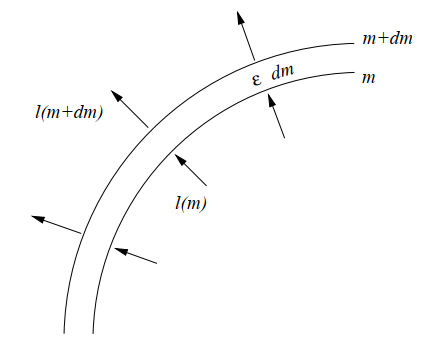
\includegraphics[scale=0.5]{Figures/thermal_equilibrium_scheme.png}
    \caption{Παραγωγή ενέργειας και ροή θερμότητας προς και από σφαιρικό φλοιό μάζας $dm$.}
    \label{fig:thermal_equilibrium_scheme}
\end{figure}

Έστω ότι θεωρούμε έναν σφαιρικό, Λαγκραντζιανό φλοιό σταθερής μάζας $dm$ μέσα σε έναν αστέρα (σχήμα \ref{fig:thermal_equilibrium_scheme}). Αλλαγές στο ποσό θερμότητας ($dQ = dq \,dm$) μπορεί να οφείλονται σε διάφορες πηγές ή καταβόθρες:
\begin{itemize}
    \item Θερμότητα εναποτίθεται από την ενέργεια που παράγουν οι πυρηνικές αντιδράσεις. Ο ρυθμός της ενέργειας ανά μονάδα μάζας και χρόνου είναι $\epsilon_{\text{nuc}}$.
    \item Θερμότητα μπορεί να διαρρέει λόγω ακτινοβολίας νετρίνο, τα οποία δεν αλληλεπιδρούν σχεδόν καθόλου με την ύλη και διαφεύγουν από την επιφάνεια του αστέρα ανεμπόδιστα. Τα νετρίνο δημιουργούνται είτε ως παράγωγα συγκεκριμένων πυρηνικών αντιδράσεων, οπότε και συνυπολογίζονται στην $\epsilon_{\text{nuc}}$, είτε λόγω ασθενών αλληλεπιδράσεων στην περίπτωση που έχουμε πολύ πυκνό και θερμό πλάσμα. Η ενέργεια που χάνεται (ανά μονάδα μάζας και χρόνου) λόγω των νετρίνο συμβολίζεται με $\epsilon_\nu$ και παίζει μεγάλο ρόλο στην ψύξη του πυρήνα σε μεταγενέστερα στάδια της εξέλιξης ενός αστέρα.
    \item Απορρόφηση ή εκπομπή θερμότητας, σύμφωνα με την ισορροπία μεταξύ της θεμικής ροή που εισέρχεται στο κατώτερο μέρος του φλοιού και της θερμικής ροής που εξέρχεται από το ανώτερο στρώμα του φλοιού. Ορίζουμε έτσι ένα νέο μέγεθος, τη \textit{τοπική λαμπρότητα} (local luminosity), ως τον ρυθμό με τον οποίο η ενέργεια με τη μορφή θερμότητας κινείται προς τα εξωτερικά στρώματα διαμέσου μιας σφαίρας ακτίνας $r$. Σε σφαιρική συμμετρία η τοπική λαμπρότητα συνδέεται με την ακτινική ροή ενέργειας $F$ μέσω της σχέσης
    \begin{equation}
        \label{eq:local_luminosity}
        l = 4\pi r^2 F
    \end{equation}
    Έτσι, η τοπική λαμπρότητα στην επιφάνεια του αστέρα είναι $l(R) = L$ και στο κέντρο του $l(0) = 0$. Φυσιολογικά, η θερμότητα ρέει προς τα έξω, προς τη κατεύθυνση δηλαδή που μειώνεται η θερμοκρασία. Γι' αυτό η τοπική λαμπρότητα είναι συνήθως θετική. Παρόλα αυτά, σε συγκεκριμένες περιπτώσεις (π.χ. ψύξη του πυρήνα λόγω ακτινοβολίας νετρίνο), η θερμότητα μπορεί να ρέει προς το εσωτερικό του αστέρα, πράγμα που σημαίνει ότι η τοπική λαμπρότητα είναι αρνητική.
\end{itemize}

Μπορούμε λοιπόν να γράψουμε:
\begin{equation*}
    \delta Q = \epsilon_{\text{nuc}} \,dm \,\delta t - \epsilon_\nu \,dm \,\delta t + l(m) \,\delta t - l(m+dm) \,\delta t
\end{equation*}
Επειδή 
\begin{equation*}
    l(m+dm) = l(m) + \frac{dl}{dm}dm    
\end{equation*}
η παραπάνω σχέση αν διαιρέσουμε και με την μάζα $dm$, γράφεται και ως
\begin{align*}
    \delta q &= \epsilon_{\text{nuc}} \,\delta t - \epsilon_\nu \,\delta t - \frac{dl}{dm} \delta t = \left(\epsilon_{\text{nuc}} - \epsilon_\nu - \frac{dl}{dm}\right) \delta t
\end{align*}
Ο δεύτερος νόμος της θερμοδυναμικής ορίζει την ειδική (specific) εντροπία, $s$, ενός συστήματος ως
\begin{eqnarray}
    \label{eq:second_law_of_thermodynamics}
    dq = Tds
\end{eqnarray}
οπότε παίρνοντας το όριο $\delta t \rightarrow 0$, καταλήγουμε στην σχέση
\begin{eqnarray}
    \label{eq:thermal_equilibrium_lagrangian_with_entropy_term}
    \boxed{\frac{dl}{dm} = \epsilon_{\text{nuc}} - \epsilon_\nu - T \frac{ds}{dt}}
\end{eqnarray}

Συνηθίζεται να γράφουμε 
\begin{equation*}
    \epsilon_{\text{gr}} = -T \frac{ds}{dt}
\end{equation*}
οπότε αν $\epsilon_{\text{gr}} > 0$, τότε ο φλοιός απελευθερώνει ενέργεια λόγω συστολής, ενώ εαν $\epsilon_{\text{gr}} < 0$, ο φλοιός απορροφά ενέργεια λόγω διαστολής. Σε θερμική ισορροπία $\epsilon_{\text{gr}} = 0$, καθώς ο αστέρας είναι σε στατική κατάσταση και άρα η χρονική παράγωγος μηδενίζεται, οπότε έχουμε την απλοποιημένη \textbf{εξίσωση θερμικής ισορροπίας} στο σύστημα συντεταγμένων του Lagrange
\begin{equation}
    \label{eq:thermal_equilibrium_lagrangian_form}
    \boxed{\frac{dl}{dm} = \epsilon_{\text{nuc}} - \epsilon_\nu}
\end{equation}
ή ισοδύναμα, στο σύστημα συντεταγμένων του Euler
\begin{equation}
    \label{eq:thermal_equilibrium_eulerian_form}
    \boxed{\frac{dl}{dr} = 4\pi r^2 \rho \left( \epsilon_{\text{nuc}} - \epsilon_\nu \right)}
\end{equation}
και αποτελεί την τρίτη βασική διαφορική εξίσωση που περιγράφει την δομή ενός αστέρα.

Ολοκληρώνοντας την σχέση \eqref{eq:thermal_equilibrium_lagrangian_form} ως προς τη μάζα, έχουμε
\begin{equation}
    \label{eq:neutrino_luminosity}
    L = \int_{0}^{M} \epsilon_{\text{nuc}} \,dm - \int_{0}^{M} \epsilon_\nu \,dm \equiv L_{\text{nuc}} - L_\nu 
\end{equation}
όπου το $L_\nu$ ορίζει την \textit{λαμπρότητα νετρίνο}. Θεωρώντας ότι $L_\nu \approx 0$, τότε ισχύει $L_{\text{nuc}} = L$, όπως δηλαδή είχαμε υποθέσει ότι ισχύει στην κατάσταση θερμικής ισορροπίας.
%% ---------------------------------------------------------------------------------------------------- %%
%% ---------------------------------------------------------------------------------------------------- %%
%% ---------------------------------------------------------------------------------------------------- %%
\subsection{Πηγές ενέργειας των αστέρων}
Στις αρχές του 20ου αιώνα, η μόνη πηγή παραγωγής ενέργειας ικανή να ερμηνεύσει τη φωτεινότητα του Ήλιου, ήταν η βαρυτική συστολή (η χημική καύση είχε ήδη απορρηφθεί ως ανεπαρκής). Η ιδέα πίσω από αυτόν τον φυσικό μηχανισμό, γνωστός και ως μηχανισμός Kelvin-Helmholtz, είναι το θεώρημα virial. Από όσα αναφέραμε, προκύπτει το συμπέρασμα ότι όταν η ακτίνα ενός αστέρας ελλατώνεται, το ίδιο συμβαίνει και με τη δυναμική του ενέργεια. Συμφωνα όμως με το θεώρημα virial, μόνο η μισή από τη δυναμική ενέργεια που απελευθερώνεται με αυτόν τον τρόπο μένει στον αστέρα με τη μορφή άτακτης κινητικής ενέργειας (θερμότητας). Η υπόλοιπη χάνεται από το σύστημα και ακτινοβολείται στο διάστημα. 
Έστω όμως ότι ο Ήλιος δεν έχει κάποια εσωτερική πηγή ενέργειας και ότι ο μηχανισμός παραγωγής ενέργειας οφείλεται στον μηχανισμό Kelvin-Helmholtz. Κατά τη γέννηση του Ήλιου από το μεσοαστρικό αέριο, είχε μάζα $\mathcal{M}$ και ακτίνα $\mathcal{R}$ αντίστοιχα. Η βαρυτική δυναμική ενέργεια τότε του Ήλιου κατά τη δημουργία του θα ήταν σύμφωνα με τη σχέση \eqref{eq:gravitational_potential_energy}
$$\mathcal{E}_{\text{gr}} = - \frac{3G \mathcal{M}^2}{5 \mathcal{R}}$$
ενώ η ολική ενέργεια σύμφωνα με το θεώρημα virial θα ειναι
$$\mathcal{E}_{\text{tot}} = - \mathcal{E}_{\text{int}} = \frac{1}{2}\mathcal{E}_{\text{gr}} = - \frac{3G \mathcal{M}^2}{10 \mathcal{R}}$$
Επειδή στο αρχικό αυτό στάδιο της δημιουργίας του αστέρα η ακτίνα $\mathcal{R} \rightarrow \infty$, συνεπάγεται ότι $\mathcal{E}_{\text{gr}} \rightarrow \infty$, και άρα η συνολική βαρυτική ενέργεια που έχει ακτινοβολήσει κατά τη διάρκεια της ζωής του μέχρι σήμερα θα είναι
\begin{equation}
    E_{\text{radiated}} = \mathcal{E}_{\text{gr}} - E_{\text{gr}} = \frac{3G M_{\odot}^2}{10 R_{\odot}}
\end{equation}
όπου τα $M_{\odot}, R_{\odot}$ αντιστοιχούν στις σημερινές τιμές. Αντικαθιστώντας αυτές τις τιμές προκύπτει ότι ο Ήλιος από την αρχή της δημιουργίας του μέχρι σήμερα θα είχε ακτινοβολήσει
$$E_{\text{radiated}} \sim 4 \times 10^{48} \,\text{erg}$$
αποκλειστικά λόγω της βαρυτικής συστολής. Υποθέτωντας ότι ακτινοβολούσε όλο αυτό το διάστημα με την ίδια λαμπρότητα $(L_{\odot} = dE/dt)$, μπορούμε να υπολογίσουμε την ηλικία του Ήλιου 
$$t_{\odot} = \frac{E_{\text{radiated}}}{L_{\odot}} \sim 10^7 \,\text{yr}$$

Οι φυσικοί του 20ου αιώνα ήδη ήξεραν, από γεωλογικές μελέτες, πως η ηλικία της Γης είναι περίπου τεσσάρων δισεκατομμυρίων ετών, άρα το παραπάνω αποτέλεσμα για την ηλικία του Ήλιου δεν μπορεί να είναι αληθές. Άρα, η βαρυτική συστολή δεν μπορεί να είναι η μοναδική πηγή ενέργειας των αστέρων. 

Σήμερα γνωρίζουμε πως συγκεκριμένες πυρηνικές αντιδράσεις θα μπορούσαν να λύσουν το πρόβλημα της παραγωγής ενέργειας των αστέρων. Ειδικότερα, η θερμοπυρηνική σύντηξη βασίζεται στην απελευθέρωση της ενέργειας σύνδεσης $Q(Z, N)$, ο οποίος έχει $Z$ πρωτόνια και $N$ νετρόνια
\begin{equation}
    \label{eq:binding_energy}
    Q(Z,N) = \underbrace{\left[ Z m_{\text{p}} + N m_{\text{n}} - m(Z,N) \right]}_{\text{έλλειμα μάζας}}c^2
\end{equation}

Ο μηχανισμός Kelvin-Helmholtz προβλέπει παραγωγή ισχύος σε όλο το εσωτερικό του αστέρα, είναι όμως σημαντικός μόνο στο στάδιο της δημιουργίας του αστέρα από τη συστολή του νέφους σκόνης και αερίου, δηλαδή πριν δημιουργηθούν οι κατάλληλες συνθήκες για τις απαραίτητες πυρηνικές αντιδράσεις. Σε έναν τυπικό αστέρα όπως αυτούς που έχουμε περιγράψει μέχρι στιγμής, η παραγωγή ενέργειας με βαρυτική συστολή είναι μηδενική. Παρόλα αυτά, υπάρχουν στάδια στην εξέλιξη ενός αστέρα όπου ο ρυθμός των πυρηνικών αντιδράσεων μειώνεται και ο μηχανισμός Kelvin-Helmoltz παίζει ενεργό ρόλο στην πορεία που θα ακολουθήσει ο αστέρας.
%% ---------------------------------------------------------------------------------------------------- %%
%% ---------------------------------------------------------------------------------------------------- %%
%% ---------------------------------------------------------------------------------------------------- %%
\subsubsection{Σύντηξη Υδρογόνου}
Το υδρογόνο είναι το στοιχείο με την μεγαλύτερη αφθονία στο σύμπαν και, μαζί με το ήλιο, είναι τα μοναδικά στοιχεία τα οποία έχουν κοσμολογική προέλευση και όχι --μόνο-- αστρική. Είναι λογικό λοιπόν και αναμενόμενο, αν λάβουμε υπόψιν την τεράστια συγκέντρωση του υδρογόνου στα άστρα μάζι με το γεγονός ότι το δυναμικό Coulomb που πρέπει να ξεπεραστεί είναι το ελάχιστο δυνατό, ότι οι αντιδράσεις θα βασίζονται σε πρώτη φάση στη σύντηξη αυτού του στοιχείου. Άρα οι αντιδράσεις που περιμένουμε να δούμε σαν οι πλέον εύκολες είναι οι:

\begin{eqnarray} \rm
p + p & \leftrightharpoons & \rm He^2 \label{eq:p+p_he2} \\ 
\rm p + He^4 & \leftrightharpoons &  \rm Li^5 \label{eq:p+he_li5} \\
\rm He^4 + He^4 & \leftrightharpoons & \rm Be^8 \label{eq:he4+he4_be8_1}
\end{eqnarray}
Παρατηρούμε ότι τα παράγωγα είναι ασταθή και άρα οι αντιδράσεις είναι αμφίδρομες. Άρα χρησιμοποιώντας μόνο τα στοιχεία που βρίσκονται σε αφθονία δεν οδηγηθήκαμε πουθενά. Χρειαζόμαστε λοιπόν έναν μηχανισμό που να επιτρέπει την μετατροπή πρωτονίων σε νετρόνια προκειμένου να οδηγηθούμε σε δημιουργία σταθερών πυρήνων. Ένας τέτοιος μηχανισμός είναι ο εξής:

\begin{eqnarray}
\rm 4p \longrightarrow \rm He^4 + 2e^{+} +2 \nu \label{eq:4p_he4}
\end{eqnarray}

Το πρόβλημα όμως εδώ είναι ότι αυτός ο μηχανισμός απαιτεί την ταυτόχρονη αλληλεπίδραση τεσσάρων πρωτονίων, πράγμα εξαιρετικό απίθανο. Ο σκόπελος αυτός ξεπεράστηκε από τους Bethe και Critchfield (H. Bethe and C. Critchfield, \textit{The formation of deuteron by proton combination}, Phys. Rev., 54:248–254, August 1938) όπου πρότειναν την μετατροπή ενός πρωτονίου σε νετρόνιο μέσω της ασθενούς αλληλεπίδρασης:

\begin{eqnarray}
\rm p + p \longrightarrow \rm d + e^{+} + \nu \label{eq:p+p_d+e}
\end{eqnarray}
Σημειώστε στο σημείο αυτό ότι, επειδή η αλληλεπίδραση αυτή γίνεται με ασθενείς δυνάμεις, η ενεργός διατομή είναι πολύ μικρή ($\sim 10^{-47}$ cm$^2$) --πολλές τάξεις μεγέθους μικρότερη από αυτές που μπορούμε να μετρήσουμε-- και αυτός είναι ο λόγος για τον οποίο το υδρογόνο καταναλώνεται με τόσο αργό ρυθμό στα άστρα (Χ. Ελευθεριάδης, \textit{Πυρηνοσύνθεση: Δημιουργία των Στοιχείων στο Σύμπαν}, Διδακτικές Σημειώσεις, Τμήμα Εκδόσεων Αριστοτέλειου Πανεπιστημίου Θεσσαλονίκης, 2010, pp. 27).

Η σειρά των αντιδράσεων που ορίζονται ως \textbf{κύκλος PPI} είναι:

\begin{eqnarray}
\rm p + p & \longrightarrow & \rm d + e^{+} + \nu  \hspace{1cm} (\times 2) \label{eq:p+p_d+e_twice}\\ 
\rm d + p & \longrightarrow & \rm He^3 + \gamma \hspace{1.5cm} (\times 2) \label{eq:d+p_he3+gamma_twice}\\
\rm He^3 + He^3 & \longrightarrow & \rm He^4 + 2p \label{eq:he3+he3_he4+2p}
\end{eqnarray}
Για θερμοκρασία της τάξης των $T \sim 10^7 \,\text{K}$, οι τυπικοί χρόνοι αντίδρασης είναι 
\begin{itemize}
    \item $14 \times 10^9 \,\text{yr}$ για την \eqref{eq:p+p_d+e_twice}
    \item $6 \,\text{s}$ για την \eqref{eq:d+p_he3+gamma_twice}
    \item $10^6 \,\text{yr}$ για την \eqref{eq:he3+he3_he4+2p}
\end{itemize}
Ο συνολικός λοιπόν ρυθμός με τον οποίο τέσσερα πρωτόνια μετατρέπονται σε ήλιο, καθορίζεται από την αρχική αντίδραση δύο πρωτονίων προς δευτέριο (bottleneck). Προσεγγιστικά, η ενέργεια που παράγεται από τον κύκλος PPI είναι
\begin{eqnarray}
    \label{eq:ppi_energy}
    \epsilon_{\text{PP}} \propto \rho \,X_{\text{H}}^2 \,T^4 
\end{eqnarray}
Η ισχυρή εξάρτηση από την θερμοκρασία είναι ο λόγος που αυτού του είδους οι αντιδράσεις χαρακτηρίζονται ως "θερμοπυρηνικές".
%% ---------------------------------------------------------------------------------------------------- %%
%% ---------------------------------------------------------------------------------------------------- %%
%% ---------------------------------------------------------------------------------------------------- %%   
\subsubsection{Καύση Δευτέριου}
Είδαμε λοιπόν ότι, το δευτέριο δημιουργείται στο εσωτερικό των αστέρων κατά βάση μέσω της αντίδρασης \eqref{eq:p+p_d+e_twice}. Η ποσότητα του δευτερίου που παράγεται είναι πολύ λίγη και το επόμενο στάδιο είναι η καύση του μέσω διάφορων αντιδράσεων είτε με πρωτόνια, είτε με άλλους πυρήνες δευτερίου είτε ακόμα και με πυρήνες ηλίου. Όμως σε ένα αστρικο περιβάλλον, η συγκέντρωση των πρωτονίων υπερτερεί κατά πολύ έναντι οποιουδήποτε άλλου είδους σωματιδίων και έχοντας κατά νου ότι ο ρυθμός αντίδρασης εξαρτάται, μεταξύ άλλων, και από το πλήθος των σωματιδίων, είναι εύλογο να υποθέσουμε ότι η καταστροφή του δευτερίου συμβαίνει μέσω της αντίδρασης:

\begin{eqnarray}
\rm d + p \longrightarrow \rm He^3 + \gamma \label{eq:d+p_he3+gamma}
\end{eqnarray}

Οι πυρήνες $^3$He που δημιουργούνται με αυτό τον τρόπο, συμβάλλουν ακόμα περισσότερο στην καταστροφή του δευτερίου μέσω των αντιδράσεων:

\begin{eqnarray}
\rm d + He^3 & \longrightarrow & \rm He^4 + p \label{eq:d+he3_he4+p}\\
\rm d + He^3 & \longrightarrow & \rm Li^5 + \gamma \label{eq:d+he3_li5+gamma}
\end{eqnarray}
Η συμβολή της \eqref{eq:d+he3_he4+p} στην καύση του δευτερίου είναι σημαντικότερη από αυτή της \eqref{eq:d+he3_li5+gamma} λόγω του ότι η ενεργός διατομή της είναι μεγαλύτερη\footnote{Η ενεργός διατομή της \eqref{eq:d+he3_he4+p} είναι ακόμα μεγαλύτερη και από αυτή της \eqref{eq:d+p_he3+gamma} όμως λόγω της ποσότητας των πρωτονίων, που είναι εξαιρετικά μεγάλος, η \eqref{eq:d+p_he3+gamma} είναι ο κύριος μηχανισμός καύσης του δευτερίου.}.

Τελικώς, επειδή η καύση του δευτερίου λαμβάνει χώρα πριν το άστρο καταφέρει να φτάσει στην κύρια ακολουθία, και λόγω του ότι η συγκέντρωση του δευτερίου είναι τόσο μικρή που γρήγορα θα καταναλωθεί, η μόνη συνέπεια είναι μία επιβράδυνση της κατάρρευσης του άστρου.
%% ---------------------------------------------------------------------------------------------------- %%
%% ---------------------------------------------------------------------------------------------------- %%
%% ---------------------------------------------------------------------------------------------------- %%
\subsubsection{Οι κύκλοι πρωτονίου-πρωτονίου}
Μέχρι στιγμής, αναφέραμε τον πρώτο κύκλο πρωτονίου-πρωτονίου (PPI) όπου στην τελευταία εξίσωση είχαμε την αντίδραση δύο πυρήνων He$^3$. Αντί γι' αυτήν την αντίδραση, μπορούμε να έχουμε την:

\begin{eqnarray}
\rm He^3 + He^4 \longrightarrow \rm Be^7 + \gamma \label{eq:he3+he4_be7+gamma}
\end{eqnarray}
και με τη σειρά του, το Be$^7$:

\begin{eqnarray}
\rm Be^7 + e & \longrightarrow & \rm Li^7 + \nu \label{eq:be7+e_li7+nu}\\
\rm Li^7 + p & \longrightarrow & \rm He^4 + \alpha \label{eq:li7+p_he4+alpha}
\end{eqnarray}
Παρατηρούμε ότι ο κύκλος αυτός, που είναι γνωστός ως \textbf{κύκλος PPII}, οδηγεί ξανά στη δημιουργία He$^4$, ενώ το Be$^7$ και το Li$^7$ δρουν απλά ως καταλύτες δεδομένου ότι δημιουργούνται και καταστρέφονται κατά τον κύκλο αυτό.

Τέλος, υπάρχει περίπτωση το Be$^7$ να αλληλεπιδράσει με ένα πρωτόνιο, πριν προλάβει να κάνει αρπαγή ηλεκτρονίου μέσω της \eqref{eq:be7+e_li7+nu}. Σε αυτή την περίπτωση έχουμε τον εξής κύκλο:

\begin{eqnarray}
\rm Be^7 + p & \longrightarrow & \rm B^8 + \gamma \label{eq:be7+p_b8+gamma}\\
\rm B^8 & \longrightarrow & \rm Be^8 + e^{+} + \nu \label{eq:b8_be8+e+nu}\\
\rm Be^8 & \longrightarrow & \rm He^4 + He^4 \label{eq:be8_he4+he4}
\end{eqnarray}
Αυτός ο κύκλος είναι γνωστός ως \textbf{κύκλος PPIII}. Παρατηρούμε ότι και εδώ το βηρύλλιο και το βόριο παίζουν το ρόλο καταλύτη.
%% ---------------------------------------------------------------------------------------------------- %%
%% ---------------------------------------------------------------------------------------------------- %%
%% ---------------------------------------------------------------------------------------------------- %%
\subsubsection{Ο κύκλος άνθρακα}
Θα περίμενε κανείς, ότι βαρύτερα στοιχεία όπως ο άνθρακας, το οξυγόνο κτλ, θα έπρεπε να έχουν μηδενική συγκέντρωση κατά τα πρώτα στάδια εξέλιξης ενός άστρου, της καύσης δηλαδή του υδρογόνου και του ηλίου. Σε γενικές γραμμές αυτό αληθεύει και η σύγκεντρωση αυτών των στοιχείων αρχίζει να γίνεται σημαντική μετά την ολοκλήρωση της καύσης του ηλίου, όμως πολλά άστρα περιέχουν τέτοια βαρύτερα στοιχεία τα οποία βρίσκονταν σε πρωτοαστρικά νέφη προερχόμενα από την εκρηκτική κατάληξη άλλων άστρων. Τα στοιχεία αυτά μπορούν να συμμετέχουν στους κύκλους των πυρηνικών καύσεων μέσω των αντιδράσεων:

\begin{eqnarray}
\rm C^{12} + p & \longrightarrow & \rm N^{13} + \gamma \label{eq:c12+p_n13+gamma}\\
N^{13} & \longrightarrow & C^{13} + e^{+} + \nu \label{eq:n13_c13+e+nu}
\end{eqnarray}

και 

\begin{eqnarray}
\rm C^{13} + p & \longrightarrow & \rm N^{14} + \gamma \label{eq:c13+p_n14+gamma}\\
\rm N^{14} + p & \longrightarrow & \rm O^{15} + \gamma \label{eq:n14+p_o15+gamma}\\     
\rm O^{15} & \longrightarrow & \rm N^{15} + e^{+} + \nu \label{eq:o15_n15+e+nu}\\
\rm N^{15} + p & \longrightarrow & \rm C^{12} + He^4 \label{eq:n15+p_c12+he4}
\end{eqnarray}
ή συνολικά:

\begin{eqnarray}
\rm C^{12} + 4p \longrightarrow \rm C^{12} + He^4 + 2e^{+} + 2 \nu \label{eq:c12+4p_c12+he4+2e+2nu}
\end{eqnarray}
όπου ο άνθρακας είναι απλά καταλύτης. Αυτός ο κύκλος είναι γνωστός ως \textbf{κύκλος άνθρακα} ή κύκλος CNO, όπου χρησιμοποιώντας ισότοπα άνθρακα, αζώτου ή οξυγόνου ως καταλύτες, παίρνουμε ήλιο-4, δύο ποζιτρόνια και δύο νετρίνο. Ο ίδιος κύκλος ισχύει για οποιοδήποτε από τα στοιχεία C, N, O κι αν θεωρήσουμε ως αρχικά παρόν αν και η παρουσία οξυγόνου περιπλέκει κάπως τα πράγματα οδηγώντας μας στον διπλό κύκλο CNO αλλά αυτό είναι ένα θέμα που δεν θα αναπτύξουμε εδώ.

Η ενέργεια που παράγεται μέσω του κύκλου άνθρακα είναι προσεγγιστικά
\begin{eqnarray}
    \label{eq:cno_energy}
    \epsilon_{\text{CNO}} \propto \rho \,X_{\text{H}} \,X_{\text{CNO}} \,T^{20} 
\end{eqnarray}
Παρατηρούμε ότι η ενέργεια που παράγεται μέσω αυτής της διαδικασίας έχει εξαιρετικά μεγάλη εξάρτηση από τη θερμοκρασία και ότι ακόμα και μικρές μεταβολές $\Delta T$, μπορεί να οδηγήσουν στην εξάλειψη αυτής της πηγής ενέργειας.
%% ---------------------------------------------------------------------------------------------------- %%
%% ---------------------------------------------------------------------------------------------------- %%
%% ---------------------------------------------------------------------------------------------------- %%
\subsubsection{Καύση Ηλίου}
Το ήλιο είναι, όπως έχουμε αναφέρει, το δεύτερο σε αφθονία στοιχείο στο Σύμπαν και έχει προέλευση τόσο κοσμολογική όσο και αστρική, μέσω των αντιδράσεων που παρουσιάσαμε στις προηγούμενες παραγράφους. Όταν λοιπόν τελειώσει η φάση της καύσης του υδρογόνου, η υδροστατική ισορροπία θα χαθεί λόγω της συνεχούς μείωσης της βαθμίδας της πίεσης και δεν θα υπάρχει τίποτα να αντισταθμίσει την βαρυτική κατάρρευση του άστρου. Έτσι, το άστρο θα συνεχίσει να καταρρέει μέχρις ότου η θερμοκρασία και η πίεση στο εσωτερικό του να επιτρέψουν την εκκίνηση των πυρηνικών μετασχηματισμών με βάση το ήλιο. Ο ρόλος του θεωρήματος virial και του μηχανισμού Kelvin-Helmholtz σε αυτό το στάδιο, δηλαδή μέχρι την εκκίνηση της καύσης του ηλίου, είναι προφανής.

Το πρόβλημα εδώ είναι, όπως αναφέρει ο Clayton, ότι δεν υπάρχουν σταθεροί πυρήνες με μαζικό αριθμό 5 και 8. Το γεγονός αυτό, απαγορεύει τόσο την σύντηξη δύο πυρήνων ηλίου μεταξύ τους όσο και την αντίδραση ενός άλφα σωματιδίου με κάποιο νουκλεόνιο. Επίσης, ο άνθρακας και το οξυγόνο (τα δύο στοιχεία που βρίσκονται σε μεγαλύτερη αφθονία μετά το ήλιο) είναι συνθέσεις τριών και τεσσάρων πυρήνων ηλίου αντίστοιχα, αλλά η αντίδραση πολλών σωματιδίων ταυτόχρονα είναι εξαιρετικά απίθανη και δεν δικαιολογεί την παρατηρούμενη αναλογιά αυτών των στοιχείων.

Εν συντομία, το πρόβλημα προσεγγίστηκε μέσω της σχέσης
\begin{eqnarray}
\rm He^4 + He^4 \leftrightharpoons \rm Be^8 \label{eq:he4+he4_be8}
\end{eqnarray}    
όπου φαίνεται ότι η αντίδραση δύο πυρήνων ηλίου δίνει το ασταθές βηρύλλιο-8. Όμως λόγω της συνεχούς δημιουργίας και καταστροφής του βηρυλλίου καθώς και του μέσου χρόνου διάσπασής του ($\sim 2.6 \times 10^{-16} \,\text{sec}$, θα υπάρχει μία ισορροπία έτσι ώστε κάθε χρονική στιγμή να υπάρχει ένας ικανοποιητικός αριθμός πυρήνων Be$^8$, έτσι ώστε να είναι πιθανή η αντίδραση:

\begin{eqnarray}
\rm Be^8 + He^4 \longrightarrow \rm C^{12} + \gamma \label{eq:be8+he4_c12+gamma}
\end{eqnarray}
η οποία παρουσιάζει κάποια χαρακτηριστικά συντονισμού.
%% ---------------------------------------------------------------------------------------------------- %%
%% ---------------------------------------------------------------------------------------------------- %%
%% ---------------------------------------------------------------------------------------------------- %%
\subsubsection{Η διαδικασία τριών-$\alpha$}
Η διαδικασία τριών-$\alpha$ είναι αυτή κατά την οποία τρεις πυρήνες ηλίου μετασχηματίζονται μέσω σύντηξης σ' ένα πυρήνα άνθρακα. Όπως αναφέρθηκε και πριν, η πιθανότητα να συμβεί μία τέτοια αντίδραση είναι εξαιρετικά μικρή και έτσι απαιτείται μεγάλο χρονικό διάστημα για να παραχθεί σημαντική ποσότητα άνθρακα μέσω αυτής. Μπορούμε εν γένει να θεωρήσουμε τις εξισώσεις \eqref{eq:he4+he4_be8} και \eqref{eq:be8+he4_c12+gamma} ως μία διαδικασία τριών-$\alpha$ δύο βημάτων. Η ενέργεια που παράγεται μέσω αυτής της διαδικασίας είναι προσεγγιστικά
\begin{eqnarray}
    \label{eq:triple_alpha_energy}
    \epsilon_{\text{3\alpha}} \propto \rho^2 \,X_{\text{He}}^3 \,T^{30} 
\end{eqnarray}

Έχοντας λύσει το πρόβλημα της δημιουργίας του άνθρακα μέσω της τριών-$\alpha$ διαδικασίας, μπορούμε να υποθέσουμε ότι το οξυγόνο σχηματίζεται μέσω της αντίδρασης:

\begin{eqnarray}
\rm C^{12} +He^4 \longrightarrow \rm O^{16} + \gamma \label{eq:c12+he4_o16+gamma}
\end{eqnarray}
και ακόμα, με ένα βήμα παραπάνω έχουμε το σχηματισμό ενός πυρήνα νέον-20 μέσω της:

\begin{eqnarray}
\rm O^{16} + He^4 \longrightarrow \rm Ne^{20} + \gamma \label{eq:o16+he4_ne20+gamma}
\end{eqnarray}

Περαιτέρω αντιδράσεις είναι σχετικά απίθανες λόγω του αυξημένου φράγματος Coulomb. Σε γενικές γραμμές, λαμβάνοντας υπόψιν τις πιθανότητες να συμβούν οι παραπάνω αντιδράσεις, είναι ασφαλές να πούμε ότι το αποτέλεσμα της καύσης του He$^4$ είναι ο σχηματισμός του άνθρακα και του οξυγόνου.
%% ---------------------------------------------------------------------------------------------------- %%
%% ---------------------------------------------------------------------------------------------------- %%
%% ---------------------------------------------------------------------------------------------------- %%
\subsubsection{Καύση Άνθρακα}
Ο αστέρας, έχοντας εξαντλήσει και τα αποθέματα του He$^4$, έχει απομείνει με τεράστιες συγκεντρώσεις άνθρακα-12 και οξυγόνο-16 στο εσωτερικό του. Για ακόμα μια φορά υπερισχύει η βαρυτική κατάρρευση του άστρου μέχρις ότου η θερμοκρασία στο κέντρο του να φτάσει την τάξη του $\sim 10^9 \,\text{K}$. Στο σημείο αυτό ξεκινούν οι αντιδράσεις μεταξύ πυρήνων άνθρακα και ακολουθούν αυτές που περιλαμβάνουν το οξυγόνο.
Από μία πληθώρα πυρηνικών αντιδράσεων μεταξύ δύο πυρήνων άνθρακα, οι πιο πιθανές να συμβούν είναι οι:

\begin{eqnarray}
\rm C^{12} + C^{12} & \longrightarrow & \rm  ^{24}Mg^{*} \longrightarrow Ne^{20} + \alpha + (4.6 \,\text{MeV}) \label{eq:c12+c12_mg24_ne20+alpha+q}\\
\rm C^{12} + C^{12} & \longrightarrow & \rm Na^{23} + p + (2.2 \,\text{MeV}) \label{eq:c12+c12_na23+p+q}
\end{eqnarray}

Αντιδράσεις μεταξύ άνθρακα και άλλων στοιχείων όπως οξυγόνο ή νέον δεν αποκλείονται, ειδικά κατά το τελευταίο στάδιο καύσης του άνθρακα, αλλά δεν κατέχουν σημαντικό ρόλο. Με παρόμοιο τρόπο γίνεται και η καύση του οξυγόνου μέσω των:

\begin{eqnarray}
\rm O^{16} + O^{16} & \longrightarrow & \rm S^{32} + \gamma  \label{eq:o16+o16_s32}\\
\rm O^{16} + O^{16} & \longrightarrow & \rm S^{31} + n \label{eq:o16+o16_s31+n}\\
\rm O^{16} + O^{16} & \longrightarrow & \rm P^{31} + p \label{eq:o16+o16_p31+p}\\
\rm O^{16} + O^{16} & \longrightarrow & \rm Si^{31} + \alpha \label{eq:o16+o16_si31+alpha}
\end{eqnarray}

Τέλος, το υπάρχον Ne$^{20}$ μπορεί να συντελέσει στην παραγωγή ενέργειας σε έναν αστέρα, για πολύ σύντομο χρονικό διάστημα ( $\sim 1 \,\text{yr}$), κυρίως μέσω αντιδράσεων φωτοδιάσπασης στις οποίες θα αναφερθούμε παρακάτω.
%% ---------------------------------------------------------------------------------------------------- %%
%% ---------------------------------------------------------------------------------------------------- %%
%% ---------------------------------------------------------------------------------------------------- %%
\subsubsection{Καύση Πυριτίου}
Μετά το τέλος της καύσης του οξυγόνου, ο πυρήνας του άστρου αποτελείται κυρίως από πυρίτιο-28. Φυσικά, το άστρο θα ακολουθήσει πάλι την γνωστή πορεία που περιλαμβάνει την συστόλη του με ταυτόχρονη αύξηση της θερμοκρασίας και της πίεσης στο εσωτερικό του, οπότε θα περίμενε κανείς να συναντήσει αντιδράσεις μεταξύ των πυρήνων πυριτίου. Κάτι τέτοιο δεν συμβαίνει όμως καθώς πριν προλάβουν να αναπτυχθούν οι κατάλληλες θερμοκρασίες, ξεκινάει η διαδικασία της \textbf{φωτοδιάσπασης} (φωτόνια τα οποία διασπούν τους πυρήνες με τους οποίους αντιδρούν) που καταστρέφει το υπάρχον πυρίτιο και διαδραματίζει ουσιαστικό λόγο στην συγκεκριμένη φάση της πυρηνοσύνθεσης.
Οι φωτοδιασπάσεις δίνουν σαν αποτέλεσμα εκπομπή σωματιδίων-α, πρωτονίων και νετρονίων και με αυτό τον τρόπο, μέσα από πολύπλοκες αντιδράσεις, οδηγούν στην δημιουργία της ονομαζόμενης \textbf{ομάδας του Fe $^{56}$} και τις αντίστοιχες ισοτοπικές αναλογίες που συναντάμε. Φαίνεται λοιπόν πως η αλυσίδα της σύνθεσης νέων στοιχείων στην καρδιά των αστέρων σπάει με τον σχηματισμό του σιδήρου. Για τον σχηματισμό χημικών στοιχείων και τις διαδικασίες που απαιτούνται, γίνεται αναφορά στο παράρτημα \ref{apx:nucleosynthesis}.

Να σημειώσουμε εδώ ότι, ο σχηματισμός των ελαφρών στοιχείων (Li, Be, B) καθώς και οι κοσμικές τους αναλογίες, δεν δικαιολογούνται από τους μηχανισμούς που περιγράψαμε μέχρι στιγμής. Αυτό συμβαίνει γιατί τα ισότοπα αυτά καταστρέφονται στις συνθήκες που επικρατούν στο εσωτερικό των αστέρων. Στο πρόβλημα αυτό θα αναφερθούμε στο παράρημα \ref{apx:nucleosynthesis}, στο υποκεφάλαιο της l-διεργασίας.
%% ---------------------------------------------------------------------------------------------------- %%
%% ---------------------------------------------------------------------------------------------------- %%
%% ---------------------------------------------------------------------------------------------------- %%
\subsection{Χαρακτηριστικοί χρόνοι}
Υπάρχουν τρεις σημαντικές χρονικές κλίμακες όταν συζητάμε την αστρική εξέλιξη. Αυτές οι χρονικές κλίμακες σχετίζονται με αλλαγές στη μηχανική δομή ενός αστέρα (που περιγράφεται από την εξίσωση κίνησης \eqref{eq:equation_of_motion_eulerian_coordinate}), με αλλαγές στη θερμική δομή του αστέρα (που περιγράφονται από το θεώρημα virial), και αλλαγές στη χημική σύσταση του αστέρα.
%% ---------------------------------------------------------------------------------------------------- %%
%% ---------------------------------------------------------------------------------------------------- %%
%% ---------------------------------------------------------------------------------------------------- %%
\subsubsection{Δυναμική χρονική κλίμακα}
Μπορούμε να αναρωτηθούμε τι θα γίνει αν η κατάσταση υδροστατικής ισορροπίας παραβιαστεί: πόσο γρήγορα θα συμβούν αλλαγές στη δομή του αστέρα; Η απάντηση δίνεται από την εξίσωση κίνησης \eqref{eq:equation_of_motion_eulerian_coordinate}. Για παράδειγμα, ας υποθέσουμε ότι η πίεση που υποστηρίζει τον αστέρα ενάντια στην βαρύτητα ξαφνικά μηδενίζεται. Όλοι οι σφαιρικοί φλοιοί τότε επιταχύνονται προς το κέντρο του αστέρα λόγω της βαρύτητας: ο αστέρας ξεκινάει να καταρρέει σε συνθήκες ελεύθερης πτώσης (free fall). Προσεγγιστικά μπορούμε να γράψουμε
\begin{align*}
    \left| \ddot{r} \right| &= - \frac{GM}{r^2} - \frac{1}{\rho} \cancelto{0}{\frac{dP}{dr}} = - g 
    \Rightarrow \frac{d^2r}{dt^2} = -g \longrightarrow \left| r \right| \approx \frac{1}{2} gt^2 
    \longrightarrow \tau_{\text{ff}} = \sqrt{\frac{2R^3}{GM}}
\end{align*}
Θεωρώντας την πυκνότητα σταθερή, $\langle \rho \rangle = \frac{3M}{4\pi R^3}$ η παραπάνω σχέση γράφεται και ως
\begin{eqnarray}
    \label{eq:dynamic_timescale}
    \tau_{\text{dyn}} = \sqrt{\frac{2R^3}{GM}} \approx  \frac{1}{2} (G \langle \rho \rangle)^{- \frac{1}{2}}
\end{eqnarray}
Φυσικά κάθε σφαιρικός φλοιός επιταχύνεται με διαφορετικό ρυθμό, οπότε η παραπάνω εκτίμηση πρέπει να εκλαμβάνεται ως μία μέση τιμή για την οποία ο αστέρας καταρρέει σε μία απόσταση $R$. Μία άλλη εκτίμηση για τον δυναμικό χρόνο μπορεί να γίνει με παρόμοιο τρόπο, θεωρώντας πως η βαρύτητα ξαφνικά εξαφανίζεται: αυτό θα μας δώσει τον χρόνο που χρειάζεται η πίεση για να διαλύσει τον αστέρα, ο οποίος είναι παρόμοιος με τον χρόνο που χρειάζεται ένα ακουστικό κύμα (άλλωστε η πίεση σχετίζεται με τα ακουστικά κύματα) να ταξιδέψει από το κέντρο μέχρι την επιφάνεια του αστέρα.

Για τον Ήλιο, προκύπτει ότι $\tau_{\text{dyn}} \approx 1600 \,\text{s}$, ή περίπου μισή ώρα. Το αποτέλεσμα αυτό έχει κάποια πολύ σημαντικά αποτελέσματα:
\begin{itemize}
    \item Οποιαδήποτε απομάκρυνση από την κατάσταση υδροστατικής ισορροπίας, πρέπει να οδηγήσει πολύ γρήγορα σε παρατηρήσιμα φαινόμενα: είτε συστολή είτε διαστολή στον δυναμικό χρόνο. Αν ο αστέρας δεν μπορεί να επανέλθει σε κατάσταση υδροστατικής ισορροπίας, θα οδηγηθεί είτε σε κατάρρευση είτε σε έκρηξη.
    \item Φυσιολογικά, η υδροστατική ισορροπία μπορεί να επανέλθει έπειτα από κάποια διαταραχή (dynamical stability). Παρόλα αυτά, διαταραχή στην υδροστατική ισορροπία μπορεί να οδηγήσει σε ταλαντώσεις μικρής κλίμακας στον δυναμικό χρόνο. Αυτές οι ταλαντώσεις έχουν παρατηρηθεί τόσο στον Ήλιο όσο και σε άλλους αστέρες, με μια περίοδο της τάξης των λεπτών στην περίπτωση του Ήλιου. Η εξίσωση \eqref{eq:dynamic_timescale} μας δείχνει ότι η περίοδος των αναπάλσεων αποτελεί ένα προσεγγιστικό μέτρο της μέσης πυκνότητας του αστέρα.
    \item Πέρα από τις όποιες ταλαντώσεις, οι αστέρες βρίσκονται εξαιρετικά κοντά σε μία κατάσταση υδροστατικής ισορροπίας αφού οποιαδήποτε διαταραχή αποσβήνεται αμέσως. Μπορούμε λοιπόν με βεβαιότητα να θεωρήσουμε πως η εξίσωση \eqref{eq:hydrostatic_equilibrium_lagrangian_coordinate} ισχύει για το μεγαλύτερο χρονικό διάστημα της ζωής τους. Οι αστέρες εξελίσσονται και γι' αυτό το λόγο δεν μπορούν να είναι εντελώς στατικοί, αλλά οι αλλαγές συμβαίνουν εξαιρετικά αργά συγκριτικά με τον δυναμικό χρόνο. Έτσι, μπορούμε να πούμε ότι εξελίσσονται ημι-στατικά (quasi-statically), δηλαδή μέσω μιας σειράς σχεδόν-τέλειων καταστάσεων υδροστατικής ισορροπίας.
\end{itemize}
%% ---------------------------------------------------------------------------------------------------- %%
%% ---------------------------------------------------------------------------------------------------- %%
%% ---------------------------------------------------------------------------------------------------- %%
\subsubsection{Θερμική χρονική κλίμακα}
Ο δεύτερος χαρακτηριστικός χρόνος περιγράφει το πόσο γρήγορα μπορούν να εμφανιστούν αλλαγές στην θερμική δομή ενός αστέρα. Συνεπάγεται λοιπόν πως είναι και η χρονική κλίμακα στην οποία ένας αστέρας ο οποίος βρίσκεται σε θερμική ισορροπία αντιδρά όταν αυτή η ισορροπία διαταράσσεται. Για να έχουμε μία εκτίμηση του μεγέθους αυτής της χρονικής κλίμακας, στρεφόμαστε στο θεώρημα virial. Είδαμε ότι ένας αστέρας χωρίς κάποια εσωτερική πηγή ενέργειας συστέλλεται ακτινοβολώντας την εσωτερική του ενέργεια:
$$L = \dot{E}_{\text{int}} = - \frac{1}{2} \dot{E}_{\text{gr}}$$
όπου η τελευταία ισότητα ισχύει για την περίπτωση του ιδανικού αερίου.
Αυτό σημαίνει ότι μπορούμε να γράψουμε
\begin{equation*}
    L = \frac{d E_{\text{int}}}{dt} = - \frac{1}{2} \frac{d E_{\text{gr}}}{dt} \longrightarrow \tau_{\text{KH}} = \frac{E_{\text{int}}}{L} = - \frac{1}{2} \frac{E_{\text{gr}}}{L}
\end{equation*}
και επειδή η βαρυτική δυναμική ενέργεια είναι, όπως έχουμε δείξει, $E_{\text{gr}} = - \frac{3GM^2}{5R}$, η παραπάνω σχέση γράφεται
\begin{equation}
    \label{eq:thermal_timescale}
    \tau_{\text{KH}} = \frac{3GM^2}{10RL} \simeq 1.5 \times 10^7 \left( \frac{M}{M_{\odot}} \right)^2 \left( \frac{R}{R_{\odot}} \right)^{-1} \left( \frac{L}{L_{\odot}} \right)^{-1} \,\text{yr}
\end{equation}
Η ποσότητα $\tau_{\text{KH}}$ εκφράζει την θερμική χρονική κλίμακα (ή κλίμακα Kelvin-Helmholtz), και εκφράζει τον χρόνο στον οποίο θα λάμβανε χώρα μία τέτοια συστολή. Για τον Ήλιο είδαμε ότι $\tau_{\text{KH}} \sim 10^7 \,\text{yr}$, που σημαίνει ότι είναι πολλές τάξεις μεγέθους μεγαλύτερη από τον δυναμικό χρόνο. Γι' αυτό το λόγο δεν υπάρχει κάποια άμεση παρατήρηση που να αποδεικνύει ότι ένας οποιοσδήποτε αστέρας βρίσκεται όντως σε κατάσταση θερμικής ισορροπίας. Οι πυρηνικές αντιδράσεις που συμβαίνουν στο κέντρο του αστέρα θα του επέτρεπαν παρόλα αυτά να βρεθεί όντως σε μία τέτοια κατάσταση. Πολλές φάσεις στην εξέλιξη ενός αστέρα, κατά τη διάρκεια των οποίων η ισχύς των πυρηνικών αντιδράσεων είναι είτε μηδενική είτε ελλιπής, λαμβάνουν χώρα σε αυτή τη θερμική χρονική κλίμακα.
%% ---------------------------------------------------------------------------------------------------- %%
%% ---------------------------------------------------------------------------------------------------- %%
%% ---------------------------------------------------------------------------------------------------- %%
\subsubsection{Πυρηνική χρονική κλίμακα}
Ένας αστέρας μπορεί να παραμείνει σε θερμική ισορροπία για όσο διάστημα το επιτρέπει το απόθεμα των πυρηνικών καυσίμων του. Η χρονική κλίμακα στην οποία εξαντλούνται τα αποθέματα του εκάστοτε πυρηνικού αποθέματος, ονομάζεται πυρηνική χρονική κλίμακα. Επειδή κατά τη διάρκεια αυτών των αντιδράσεων, ένα στοιχείο μετατρέπεται σε κάποιο άλλο (π.χ. υδρογόνο σε ήλιο), είναι επίσης η χρονική κλίμακα στην οποία αλλάζει η χημική σύσταση του εσωτερικού του αστέρα.

Η πηγή ενέργειας της θερμοπυρηνικής σύντηξης είναι η μετατροπή μέρους της μάζας των αντιδρώντων σωματιδίων σε ενέργεια, έτσι ώστε $E_{\text{nuc}} = \Delta m \,c^2$, όπου $\Delta m$ το έλλειμα μάζας.
Σε κατάσταση θερμικής ισορροπίας ισχύει
$$L = L_{\text{nuc}} = \dot{E}_{\text{nuc}} = \frac{d E_{\text{nuc}}}{dt}$$
έτσι ώστε η πυρηνική χρονική κλίμακα να ορίζεται ως
\begin{equation}
    \label{eq:nuclear_timescale}
    \tau_{\text{nuc}} = \frac{E_{\text{nuc}}}{L} = \eta f_{\text{c}} X \frac{M c^2}{L} = \eta X \frac{M_{\text{c}} c^2}{L}
\end{equation}
όπου $\eta$ είναι ένας παράγοντας απόδοσης της θερμοπυρηνικής σύντηξης (για το υδρογόνο $\eta \sim 0.7 \,\%$), $f_{\text{c}}$ είναι το ποσοστό της μάζας του αστέρα στο οποίο πραγματοποιούται αντιδράσεις (για άστρα σαν τον Ήλιο είναι $\sim 10 \,\%$), $X$ η αφθονία του υδρογόνου, και $M$ η συνολική μάζα του αστέρα. Με $M_{\text{c}}$ συμβολίζουμε τη μάζα του πυρήνα του αστέρα, δηλαδή τη μάζα εκείνη που συμμετέχει στις πυρηνικές αντιδράσεις.

Για τον Ήλιο, $\tau_{\text{nuc}} \sim 10^{10} \,\text{yr}$ που είναι τάξεις μεγέθους μεγαλύτερη από την θερμική χρονική κλίμακα. Άρα, η υπόθεση ότι τα αστέρια μπορούν να φτάσουν μία κατάσταση θερμικής ισορροπίας είναι βάσιμη.

Γενικά λοιπόν ισχύει
\begin{equation}
    \label{eq:stellar_timescales_order}
    \tau_{\text{nuc}} \gg \tau_{\text{KH}} \gg \tau_{\text{dyn}}
\end{equation}
Ως αποτέλεσμα, ο ρυθμός των πυρηνικών αντιδράσεων καθορίζει το βήμα της αστρικής εξέλιξης, και οι αστέρες μπορεί να θεωρηθεί ότι βρίσκονται σε υδροστατική και θερμική ισορροπία για το μεγαλύτερο μέρος της ζωής τους.
%% ---------------------------------------------------------------------------------------------------- %%
%% ---------------------------------------------------------------------------------------------------- %%
%% ---------------------------------------------------------------------------------------------------- %%
\subsection{Διάδοση ενέργειας στους αστέρες}
Η διάδοση της ενέργειας σε ένα φυσικό σύστημα μπορεί να γίνει γενικά με τρεις τρόπους: με \textbf{αγωγή} (conduction), με \textbf{ρεύματα μεταφοράς} (convection) ή με \textbf{ακτινοβολία} (radiation). Ο συντελεστής θερμικής αγωγιμότητας των αερίων, όταν η πίεσή τους δεν είναι εξαιρετικά μεγάλη, είναι μηδαμινός. Έτσι, με εξαίρεση τους πυρήνες των πολύ μεγάλων, σε μάζα, αστέρων, των λευκών νάνων και των αστέρων νετρονίων, όπου η πίεση παίρνει ακραίες τιμές, θεωρούμε ότι η διάδοση ενέργειας μέσω αγωγής δεν είναι σημαντική συγκριτικά με τους άλλους δύο τρόπους. Επειδή οι μικροφυσικές διεργασίες στις οποίες βασίζονται οι δύο αυτοί τρόποι είναι εντελώς διαφορετικές, δεν πρέπει να μας εκπλήσσει το γεγονός ότι και η μακροσκοπική μαθηματική τους περιγραφή οδηγεί σε δύο διαφορικές εξισώσεις με εντελώς διαφορετική μαθηματική δομή.

Τα ρεύματα μεταφοράς είναι ο κύριος τρόπος διάδοσης της ενέργειας στους ψυχρούς αστέρες φασματικού τύπου Κ και Μ, συνεισφέρει όμως λιγότερο σε αστέρες όπως ο Ήλιος και σχεδόν καθόλου σε αστέρες προγενέστερου φασματικού τύπου. Η ακτινοβολία είναι ο κύριος τρόπος διάδοσης της ενέργειας στους θερμούς αστέρες καθώς και στα βαθύτερα στρώματα των ψυχρών αστέρων.
%% ---------------------------------------------------------------------------------------------------- %%
%% ---------------------------------------------------------------------------------------------------- %%
%% ---------------------------------------------------------------------------------------------------- %%
\subsubsection{Διάδοση ενέργειας με ακτινοβολία}
Η ιδέα πίσω από την διάδοση της ενέργειας με ακτινοβολία είναι ότι θερμικά φωτόνια τα οποία εκπέμπφθηκαν σε θερμές περιοχές και απορροφήθηκαν σε ψυχρότερες περιοχές, μεταφέρουν ενέργεια από την θερμή στην ψυχρή περιοχή. Η αποτελεσματικότητα αυτής της μεταφοράς ενέργειας θα είναι συνάρτηση, μεταξύ άλλων, της θερμοβαθμίδας (temperature gradient) και της ικανότητας των φωτονίων να ταξιδέψουν ελεύθερα από μία περιοχή του αστέρα σε μία άλλη. Γνωρίζουμε ότι τα φωτόνια στο εσωτερικό των αστέρων όπως ο Ήλιος, διαγράφουν μία απόσταση της τάξης του $1 \,\text{cm}$ πριν αλληλεπιδράσουν με την ύλη (μέση ελεύθερη διαδρομή, $\ell \sim 1 \,\text{cm}$), άρα η διάδοση ενέργειας μέσω ακτινοβολίας οφείλεται στην όποια διαφορά θερμοκρασίας υπάρχει μεταξύ κομματιών ύλης που βρίσκονται σε απόσταση περίπου ενός εκατοστού μεταξύ τους. Για τον Ήλιο, αυτή η διαφορά θερμοκρασίας είναι της τάξης $\Delta T \sim 10^{-4} \,\text{K}$. Η ύπαρξη κάποιας θερμοβαθμίδας είναι απαραίτητη συνθήκη για τη διάδοση θερμικής ενέργειας μέσω ακτινοβολίας, καθώς σε αντίθετη περίπτωση, και αν η ύλη βρίσκεται σε θερμοδυναμική ισορροπία, η πυκνότητα των φωτονίων σε όλες τις συχνότητες είναι ισοτροπική και άρα δεν μπορεί να υπάρξει ροή ακτινοβολίας σε καμία κατεύθυνση. Αυτή η μικρή ανισοτροπία $\frac{\Delta T}{T} \sim 10^{-11}$ είναι υπεύθυνη για την διάδοση όλη της ενέργειας του Ήλιου μέσω ακτινοβολίας.

\begin{figure}[h]
    \centering
    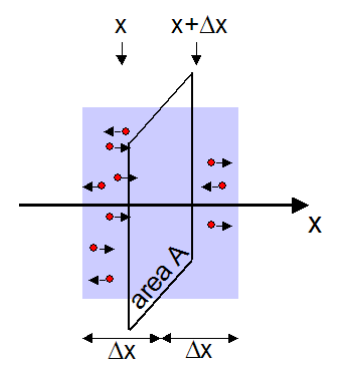
\includegraphics[scale=0.7]{Figures/ficks_diffusion_law.png}
    \caption{Τυχαία κίνηση σωματιδίων σε μία διάσταση, διερχόμενα από επιφάνεια $A$.}
    \label{fig:ficks_diffusion_law}
\end{figure}

Η διάδοση ενέργειας με ακτινοβολία μπορεί να προσεγγιστεί ως μια διαδικασία διάχυσης (diffusion) όπως θα δείξουμε. Έστω μοναδιαία επιφάνεια και σωματίδια (π.χ. φωτόνια) τα οποία διέρχονται διαμέσου αυτής της επιφάνειας κατά μία διεύθυνση $x$ (στην περίπτωσή μας αυτή η διεύθυνση θα ήταν η ακτινική και το $\Delta x = \ell$), όπως φαίνεται στο σχήμα \ref{fig:ficks_diffusion_law}. Αριστερά της επιφάνειας η αριθμητική πυκνότητα των σωματιδίων είναι $n(x)$ και δεξιά $n(x+\Delta x)$. Υποθέτοντας ότι οι ταχύτητες στις τρεις διευθύνσεις του χώρου είναι κατανεμημένες ισοτροπικά ώστε $u_x = u_y = u_z$, προκύπτει ότι για μία από τις τρεις διευθύνσεις, $u_x = \frac{1}{3} \langle u \rangle$. Το ερώτημα είναι πόσα σωματίδια διέρχονται από την επιφάνεια $A$. Διαστασιακά, η ροή των σωματιδίων μπορεί να γραφτεί ως $F = n \,u$, και επειδή τα σωματίδια έχουν την ίδια πιθανότητα να κινούνται είτε προς τα αριστερά είτε προς τα δεξιά, τα μισά σωματίδια θα κινούνται προς τη μία κατεύθυνση και τα άλλα μισά προς την άλλη. Έτσι, η ροή για τα σωματίδια που κινούνται διαμέσου της επιφάνειας $A$, από τα αριστερά προς τα δεξιά θα είναι
\begin{equation*}
    F(x) = \frac{1}{2} n(x) \,\frac{1}{3} \langle u \rangle = \frac{1}{6} n(x) \,\langle u \rangle
\end{equation*}
Αντίστοιχα, η ροή των σωματιδίων που κινούνται διαμέσου της επιφάνειας $A$, από τα δεξιά προς τα αριστερά θα είναι
\begin{equation*}
    F(x + \Delta x) = \frac{1}{6} n(x+\Delta x) \,\langle u \rangle
\end{equation*}
Έτσι, η θετική (net) ροή θα είναι
\begin{equation*}
    F = \frac{1}{6} \langle u \rangle \left[ n(x+\Delta x) - n(x) \right]
\end{equation*}
Επειδή οι αριθμοί $n(x), \,n(x + \Delta x)$ δεν είναι σταθεροί αλλά μεταβάλλονται ανάλογα με τον αριθμό των σωματιδίων που διαπερνούν την επιφάνεια και καταλήγουν είτε αριστερά είτε δεξιά, η τελευταία σχέση γράφεται
\begin{align}
    \nonumber F &= \frac{1}{6} \langle u \rangle \left[ n - \frac{dn}{dx}\Delta x - \left( n + \frac{dn}{dx}\Delta x \right) \right] = - \frac{1}{3} \langle u \rangle \Delta x \frac{dn}{dx} \Rightarrow \\ \nonumber \\
    &\Rightarrow F = -D \frac{dn}{dx}
\end{align}
όπου ο συντελεστής $D = \frac{1}{3} \langle u \rangle \Delta x$ ονομάζεται "διαχυσιμότητα" (diffusivity) και αποτελεί μέτρο του ρυθμού με τον οποίο τα σωματίδια διασκορπίζονται. Το παραπάνω αποτέλεσμα γενικεύεται στις τρεις διαστάσεις
\begin{equation}
    \label{eq:ficks_diffusion_law}
    F = - D \nabla n
\end{equation}
και είναι γνωστό ως \textbf{νόμος διάχυσης του Fick}.

Αντί της αριθμητικής πυκνότητας $n$, μπορούμε να γράψουμε κατά αντιστοιχία ότι η ροή ενέργειας λόγω διάχυσης είναι
\begin{equation}
    \label{eq:energy_density_diffusion}
    F = -D \nabla u \xrightarrow{1D} F = -D \frac{du}{dr}
\end{equation}
όπου $u$ η πυκνότητα ενέργειας. Χρησιμοποιοώντας τον κανόνα αλυσίδας $\frac{du}{dT} \,\frac{dT}{dr}$, μπορούμε να γράψουμε την σχέση \eqref{eq:energy_density_diffusion} ως
\begin{equation}
    \label{eq:temperature_gradient_diffusion_law}
    F = -D \underbrace{\frac{du}{dT}}_{= \,C_{\text{V}}} \,\frac{dT}{dr} = - K\frac{dT}{dr} \xrightarrow{3D} \boxed{F = -K \nabla T}
\end{equation}
όπου ο συντελεστής 
\begin{equation}
    \label{eq:conductivity_diffusion_coefficient}
    K = \frac{1}{3} \langle u \rangle \ell C_{\text{V}} = \frac{1}{3 \kappa_\nu \rho} \langle u \rangle C_{\text{V}}
\end{equation}
ονομάζεται "αγωγιμότητα" (conductivity) και 
\begin{equation}
    \label{eq:specific_heat_capacity}
    C_{\text{V}} = \left( \frac{du}{dT} \right)_{\text{V}}
\end{equation}
η ειδική θερμοχωρητικότητα (specific heat capacity). Αυτή η περιγραφή ισχύει για όλα τα σωματίδια σε τοπική θερμοδυναμική ισορροπία, συμπεριλαμβανομένων και των φωτονίων. 

Για ένα αέριο φωτονίων, μπορούμε να θέσουμε $\langle u \rangle = c$, όπου $c$ η ταχύτητα του φωτός στο κενό. Η πυκνότητα ενέργειας δίνεται από τη σχέση \eqref{eq:photon_energy_density} και άρα η ειδική θερμοχωρητικότητα είναι
\begin{equation*}
    C_{\text{V}} = \left( \frac{du}{dT} \right)_{\text{V}} = 4 \alpha T^3
\end{equation*}
ενώ η μέση ελεύθερη διαδρομή σχετίζεται με την αδιαφάνεια μέσω της σχέσης \eqref{eq:mean_free_path}, όπου αν πάρουμε την μέση τιμή για όλες τις συχνότητες ($\langle \kappa \rangle \equiv \kappa$) μπορεί να γραφτεί
\begin{equation*}
    \ell_{\text{ph}} = \frac{1}{\kappa \rho}
\end{equation*}
Συνδυάζοντας όλα τα παραπάνω, μπορούμε να γράψουμε τον \textbf{συντελεστή αγωγιμότητας ακτινοβολίας} \eqref{eq:conductivity_diffusion_coefficient} ως
\begin{equation}
    \label{eq:radiation_conductivity_coefficient}
    K_{\text{rad}} = \frac{4}{3} \frac{\alpha \,c \,T^3}{\kappa \rho}
\end{equation}

Σε αυτό το σημείο αξίζει να αναφέρουμε ότι και η διάδοση ενέργειας μέσω αγωγής μπορεί να περιγραφεί ως μία διαδικασία διάχυσης με την ίδια συναρτησιακή μορφή της σχέσης \eqref{eq:temperature_gradient_diffusion_law} ώστε η συνδυαστική ροή ενέργειας να είναι
\begin{equation}
    \label{eq:radiative_and_conduction_flux}
    F = - \frac{4\alpha c T^3}{3\rho}\left( \frac{1}{\kappa_{\text{rad}}} + \frac{1}{\kappa_{\text{cd}}} \right) \nabla T
\end{equation}
όπου ορίσαμε την \textbf{αδιαφάνεια αγωγής}, $\kappa_{\text{cd}}$, σε αναλογία με την αδιαφάνεια ακτινοβολίας $\kappa_{\text{rad}}$. Αυτό το αποτέλεσμα σημαίνει απλά ότι ο μηχανισμός διάδοσης ενέργειας με τη μεγαλύτερη ροή θα είναι ο κυριάρχος, ή με άλλα λόγια, ο μηχανισμός για τον οποίο η αστρική ύλη παρουσιάζει τη μεγαλύτερη διαφάνεια.

Για έναν σφαιρικά συμμετρικό αστέρα, η τοπική λαμπρότητα σχετίζεται με την ροή μέσω της σχέσης 
$$F = \frac{l}{4\pi r^2}$$
και άρα η εξίσωση \eqref{eq:radiative_and_conduction_flux} γράφεται
\begin{align}
    \label{eq:energy_transport_radiation_eulerian_diff}
    \nonumber F_{\text{rad}} &= - \frac{4}{3} \frac{\alpha \,c \,T^3}{\kappa_{\text{rad}} \rho} \frac{dT}{dr} = \frac{l}{4\pi r^2} \Rightarrow \\ \nonumber \\
    &\Rightarrow \boxed{\frac{dT}{dr} = - \frac{3\kappa \rho}{16 \pi \alpha c T^3} \frac{l}{r^2}}
\end{align}
ή στο σύστημα συντεταγμένων του Lagrange
\begin{equation}
    \label{eq:energy_transport_radiation_lagrangian_diff}
    \boxed{\frac{dT}{dm} = - \frac{3}{64\pi^2 \alpha c} \frac{\kappa l}{r^4 T^3}}
\end{equation}
Αυτή είναι η θερμοβαθμίδα που απαιτείται ώστε όλη η λαμπρότητα $l$ να μεταφερθεί μέσω ακτινοβολίας και αποτελεί την τέταρτη διαφορική εξίσωση που περιγράφει τη δομή ενός αστέρα στην περίπτωση που έχουμε διάδοση ενέργειας μόνο μέσω ακτινοβολίας. Ένα αστέρι ή μια περιοχή ενός αστεριού στην οποία ισχύει αυτή η εξίσωση ονομάζεται ζώνη ακτινοβολίας (radiative).

Η εξίσωση \eqref{eq:energy_transport_radiation_lagrangian_diff} ισχύει όσο $\ell_{\text{ph}} \ll R$, δηλαδή όσο υπάρχει τοπική θερμοδυναμική ισορροπία. Αυτή η συνθήκη σταματάει να ισχύει όσο πλησιάζουμε την επιφάνεια του αστέρα, την φωτόσφαιρα, από την οποία διαφεύγουν φωτόνια ($\ell_{\text{ph}} \gtrsim R$). Κοντά στην φωτόσφαιρα, η προσέγγιση της διάχυσης παύει να ισχύει και πρέπει να λύσουμε την --πολύ πιο δύσκολη-- εξίσωση μεταφοράς. Ευτυχώς, συνθήκες τοπικής θερμοδυναμικής ισορροπίας και η προσέγγιση της διάχυσης ισχύουν σχεδόν για όλο το εσωτερικό των αστέρων.

Για έναν αστέρα που βρίσκεται σε υδροστατική ισορροπία, μπορούμε συνδυάζοντας τις εξισώσεις \eqref{eq:hydrostatic_equilibrium_lagrangian_coordinate} και \eqref{eq:energy_transport_radiation_lagrangian_diff} να γράψουμε την θερμοβαθμίδα ως
\begin{equation*}
    \frac{dT}{dm} = \frac{dP}{dm} \,\frac{dT}{dP} = - \frac{Gm}{4\pi r^4} \,\frac{T}{P} \,\frac{d\log T}{d\log P}
\end{equation*}
ώστε να ορίσουμε την αδιάστατη θερμοβαθμίδα ακτινοβολίας (radiative temperature gradient)
\begin{eqnarray}
    \label{eq:radiative_temperature_gradient}
    \nabla_{\text{rad}} = \left(\frac{d\log T}{d\log P} \right)_{\text{rad}} = \frac{3}{16\pi \alpha c G} \frac{\kappa l P}{m T^4}
\end{eqnarray}
Η σχέση \eqref{eq:radiative_temperature_gradient} περιγράφει την λογαριθμική μεταβολή της θερμοκρασίας με το βάθος (όπου το βάθος είναι εκφρασμένο μέσω της πίεσης) σε έναν αστέρα σε υδροστατική ισορροπία, αν η ενέργεια μεταφέρεται μόνο μέσω ακτινοβολίας.
%% ---------------------------------------------------------------------------------------------------- %%
%% ---------------------------------------------------------------------------------------------------- %%
%% ---------------------------------------------------------------------------------------------------- %%
\subsubsection{Η αδιαφάνεια στο εσωτερικό των αστέρων}
Οι εξισώσεις που περιγράφουν την διάχυση της ακτινοβολίας είναι ανεξάρτητες της συχνότητας $\nu$, αφού η ροή $F$ ολοκληρώνεται ως προς όλες τις συχνότητες. Γενικά όμως, ο συντελεστής αδιαφάνειας $\kappa_\nu$ εξαρτάται από την συχνότητα, οπότε η ποσότητα $\kappa$ που εμφανίζεται στην σχέση \eqref{eq:energy_transport_radiation_lagrangian_diff}
πρέπει να παριστάνει έναν μέσο όρο ως προς τη συχνότητα.

Αν με $F_\nu d\nu$ θεωρήσουμε την ροή ακτινοβολίας στο διάστημα συχνοτήτων $[\nu, \nu+d\nu]$, τότε η εξίσωση \eqref{eq:ficks_diffusion_law} πρέπει να αντικατασταθεί με
\begin{equation}
    \label{eq:ficks_diffusion_law_frequency_dependent}
    F_\nu = -D_\nu \nabla u_\nu = -D_\nu \frac{\partial u_\nu}{\partial T} \nabla T
\end{equation}
όπου $D_\nu = \frac{1}{3} c l_{\text{ph}} = \frac{c}{3 \kappa_nu \rho}$.  Επειδή θεωρούμε ότι η ακτινοβολία βρίσκεται σε θερμική ισορροπία με το αέριο, η πυκνότητα ενέργειας στο ίδιο διάστημα, συνδέεται με την ένταση της ακτινοβολίας που δίνεται από τον νόμο του Planck μεσω της σχέσης
\begin{equation}
    \label{eq:energy_density_intensity_correlation}
    B_\nu (T) = \frac{u_\nu (T) \,c}{4\pi}
\end{equation}
Η ολική ροή προκύπτει από την ολοκλήρωση της σχέσης \eqref{eq:ficks_diffusion_law_frequency_dependent} σε όλες τις συχνότητες
\begin{equation*}
    F = - \left[\frac{c}{3 \rho} \int_{0}^{\infty} \frac{1}{\kappa_\nu} \frac{\partial u_{\nu}}{\partial T} d\nu \right] \nabla T
\end{equation*}
η οποία έχει την ίδια μορφή με τη σχέση \eqref{eq:temperature_gradient_diffusion_law} όπου 
\begin{equation*}
    K_{\text{rad}} = \frac{c}{3 \rho} \int_{0}^{\infty} \frac{1}{\kappa_\nu} \frac{\partial u_{\nu}}{\partial T} d\nu
\end{equation*}
Συγκρίνοντας το παραπάνω αποτέλεσμα με τη σχέση \eqref{eq:radiation_conductivity_coefficient} καταλήγουμε ότι
\begin{equation}
    \frac{1}{\kappa} = \frac{1}{4\alpha T^3} \int_{0}^{\infty} \frac{1}{\kappa_\nu} \frac{\partial u_{\nu}}{\partial T} d\nu
\end{equation}
όπου ο παράγοντας $4 \alpha T^3$ ισούται με $\int_{0}^{\infty} \frac{\partial u_\nu}{\partial T} d\nu$ ώστε η παραπάνω σχέση να γράφεται γενικά
\begin{equation}
    \label{eq:rosseland_mean_opacity_energy_density}
    \frac{1}{\kappa} = \frac{\int_{0}^{\infty} \frac{1}{\kappa_\nu} \frac{\partial u_{\nu}}{\partial T} d\nu}{\int_{0}^{\infty} \frac{\partial u_\nu}{\partial T} d\nu}
\end{equation}
Η ποσότητα $\kappa$ ονομάζεται \textbf{μέση αδιαφάνεια κατά Rosseland} και είναι η αρμονική μέση τιμή της αδιαφάνεια ενός αερίου συγκεκριμένης σύστασης, θερμοκρασίας και πυκνότητας, ως προς όλες τις συχνότητες της ακτινοβολίας που απορροφάται ή σκεδάζεται (σταθμισμένη με στατιστικό βάρος τη συνάρτηση $\partial u_\nu / \partial T$). Συχνά η μέση αδιαφάνεια κατά Rosseland εμφανίζεται με τον όρο της έντασης της ακτινοβολίας αντί της πυκνότητας ενέργειας, ώστε χρησιμοποιώντας την σχέση \eqref{eq:energy_density_intensity_correlation} να γράφεται και
\begin{equation*}
    \frac{1}{\kappa} = \frac{\pi}{\alpha c T^3} \int_{0}^{\infty} \frac{1}{\kappa_\nu} \frac{\partial B_{\nu} (T)}{\partial T} d\nu
\end{equation*}
ή γενικά

\begin{equation}
    \label{eq:rosseland_mean_opacity_intensity}
    \boxed{\frac{1}{\kappa} \int_{0}^{\infty} \frac{\partial B_{\nu} (T)}{\partial T} d\nu = \int_{0}^{\infty} \frac{1}{\kappa_\nu} \frac{\partial B_{\nu} (T)}{\partial T} d\nu}
\end{equation}

Όταν μελετάμε το εσωτερικό των αστέρων, δεν ενδιαφερόμαστε ιδιαίτερα για την ειδική ένταση $I_\nu$ (και την αντίστοιχη λαμπρότητα $L_\nu$), αφού δεν είναι δυνατόν να παρατηρήσουμε την κατανομή της λαμπρότητας με τη συχνότητα. Αντίθετα, ενδιαφερόμαστε για την ολική λαμπρότητα, $L$, η οποία συνδέεται άμεσα με το ενεργειακό ισοζύγιο του αστέρα (αφού σε κατάσταση ισορροπίας, η ενέργεια που ακτινοβολείται ως λαμπρότητα αναπληρώνεται από τις πηγές ενέργειας του αστέρα). Η μέση αδιαφάνεια κατά Rosseland είναι χρήσιμη όταν θέλουμε να υπολογίσουμε τη συνολική ενέργεια που απορροφήθηκε σε όλα τα μήκη κύματος, κάτι που απαιτείται στους υπολογισμούς της αστρικής δομής.


Ο συντελεστής αδιαφάνειας στο εσωτερικό των αστέρων οφείλεται στους μηχανισμούς που περιγράψαμε στο Κεφάλαιο \ref{ch:Chapter4}, δηλαδή σε φωτοϊονισμό (bound-free transition), σε πέδηση (free-free transition) ή σε σκεδάσεις (Thomson και Compton). Ο συντελεστής αδιαφάνειας που οφείλεται σε σκεδάσεις φωτονίων από ηλεκτρόνια, $\kappa_{\text{scat}}$, αποδεικνύεται ότι εξαρτάται μόνο από τη χημική σύσταστη της ύλης του αστέρα, και δίνεται από τη σχέση
\begin{equation}
    \label{eq:opacity_scattering}
    \kappa_{\text{scat}} = 0.2 (1+X) \,\text{cm$^2$/gr}
\end{equation}
όπου $X$ είναι η περιεκτικότητα της ύλης σε υδρογόνο. Παρατηρούμε ότι ο συντελεστής απορρόφησης λόγω σκέδασης από ηλεκτρόνια είναι ανεξάρτητος από τη συχνότητα των φωτονίων.

Οι συντελεστές απορρόφησης των δύο άλλων μηχανισμών, $\kappa_{\nu}^{\text{bf}}$ και $\kappa_{\nu}^{\text{ff}}$, είναι συναρτήσεις \textit{και} της συχνότητας, και επομένως χρειαζόμαστε τις αντίστοιχες αδιαφάνειες κατά Rosseland, $\kappa_{\text{bf}}$ και $\kappa_{\text{ff}}$. Αυτές έχουν υπολογιστεί από τον Kramer και δίνονται από τις σχέσεις
\begin{align}
    \kappa_{\text{bf}} &= a(X,Z,g_a,t) \rho T^s \label{eq:opacity_bound_free} \\ \nonumber \\
    \kappa_{\text{ff}} &= b(X,Z,g_b) \rho T^s \label{eq:opacity_free_free}
\end{align}
όπου ο εκθέτης, $s$, είναι συνάρτηση της θεμοκρασίας. Για τις υψηλές θερμοκρασίες που επικρατούν στο εσωτερικό των αστέρων ($T \geq 10^5$) αποδεικνύεται ότι $s = -3.5$, ενώ για σχετικά χαμηλές θερμοκρασίες ($T \approx 10^4$) αποδεικνύεται ότι $s = 10$. Οι συναρτήσεις $a, b$, στην περίπτωση που $s=-3.5$, ορίζονται από τις σχέσεις
\begin{align}
    a &= 4.34 \times 10^{25} \,\frac{g_a}{t} Z(1 + X) \label{eq:gaunt_factor_bf} \\ \nonumber \\
    b &= 3.68 \times 10^{22} \,g_b (1 + X) (1 - Z) \label{eq:gaunt_factor_ff}
\end{align}
Στις παραπάνω σχέσεις, οι συντελεστές $g_a, g_b$ και $t$ ονομάζονται \textbf{συντελεστές Gaunt} και \textbf{συντελεστής αποκοπής} (guillotine factor) αντίστοιχα. Οι συντελεστές Gaunt διορθώνουν τις αποκλίσεις μεταξύ της κλασικής και κβαντομηχανικής λύσης, ενώ ο συντελεστής αποκοπής διορθώνει τα σφάλματα των προσεγγίσεων κατά τον υπολογισμό της σχέσης \eqref{eq:gaunt_factor_bf}. Συνηθισμένες τιμές για τους συντελεστές αυτούς είναι $g_a \approx g_b \approx 3$ και $t \approx 10$. Το $X$ αντιπροσωπεύει την περιεκτικότητα (κατά μάζα) της ύλης του αστέρα σε υδρογόνο και το $Z$ την περιεκτικότητα της ύλης του αστέρα σε στοιχεία βαρύτερα από το ήλιο ("μέταλλα"), γι΄ αυτό και ονομάζεται και "metallicity".

Είθισται, οποιαδήποτε σχέση για την αδιαφάνεια έχει τη μορφή
\begin{equation}
    \label{eq:kramers_opacity_law_form}
    \kappa \propto \rho T^{-7/2}
\end{equation}
να ονομάζεται \textbf{αδιαφάνεια κατά Kramer}.

Από τους ορισμούς των $\kappa_{\text{bf}}, \kappa_{\text{ff}}$ παρατηρούμε ότι η αδιαφάνεια κατά Kramer είναι φθίνουσα συνάρτητη της θερμοκρασίας. Έτσι, σε αρκετά μεγάλες θερμοκρασίες ($T > 10^8 \,\text{K}$) η τιμή της τείνει στο μηδέν και επομένως γίνεται μικρότερη από την αδιαφάνεια σκέδασης απο ηλεκτρόνια $\kappa_{\text{scat}}$ (που είναι ανεξάρτητη της θερμοκρασίας). Από το αποτέλεσμα αυτό συμπεραίνουμε ότι η αδιαφάνεια κατά Kramer (μηχανισμοί bound-free και free-free) κυριαρχεί στους (ψυχρότερους) αστέρες μεταγενέστερων φασματικών τύπων, ενώ η αδιαφάνεια σκέδασης από ηλεκτρόνια κυριαρχεί στους (θερμότερους) αστέρες των προγενέστερων φασματικών τύπων.
%% ---------------------------------------------------------------------------------------------------- %%
%% ---------------------------------------------------------------------------------------------------- %%
%% ---------------------------------------------------------------------------------------------------- %%
\subsubsection{Το όριο Eddington}
Είδαμε ότι η διάδοση ενέργειας μέσω ακτινοβολίας μέσα σε έναν αστέρα απαιτεί μία θερμοβαθμίδα $dT/dr$, το μέγεθος της οποίας δίνεται από την εξίσωση \eqref{eq:energy_transport_radiation_eulerian_diff}. Η πίεση της ακτινοβολίας δίνεται από τη σχέση \eqref{eq:radiation_pressure_black_body} και άρα η βαθμίδα της πίεσης της ακτινοβολίας είναι
\begin{equation}
    \label{eq:radiation_pressure_gradient}
    \frac{dP_{\text{rad}}}{dr} = \frac{4}{3} \alpha T^3 \,\frac{dT}{dr} = - \frac{\kappa \rho}{4\pi c} \frac{l}{r^2}
\end{equation}
Αυτή η πίεση της ακτινοβολίας παριστάνει μία δύναμη που ασκείται προς το εξωτερικό του αστέρα λόγω της ροής των φωτονίων προς αυτή την κατεύθυνση. Φυσικά, για έναν αστέρα που βρίσκεται σε υδροστατική ισορροπία, αυτή η δύναμη πρέπει να είναι μικρότερη από τη δύναμη της βαρύτητας, όπως αυτή δίνεται από τη βαθμίδα της πίεσης που είναι απαραίτητη για την εδραίωση της υδροστατικής ισορροπίας (σχέση \ref{eq:hydrostatic_equilibrium_eulerian coordinates}). Αυτό σημαίνει ότι
\begin{align}
    \label{eq:eddington_limit}
    \nonumber \left| \frac{dP_{\text{rad}}}{dr} \right| &< \left| \left( \frac{dP}{dr} \right)_{\text{HE}} \right| \Rightarrow \frac{\kappa \rho}{4 \pi c} \frac{l}{r^2} < \frac{G m \rho}{r^2} \\ \nonumber \\
    &\Rightarrow l < \frac{4\pi G m c}{\kappa} = l_{\text{Edd}}
\end{align}
Η ποσότητα $l_{\text{Edd}} = \frac{4\pi G m c}{\kappa}$ ονομάζεται (τοπική) \textbf{λαμπρότητα Eddington} και παριστάνει τη μέγιστη λαμπρότητα που μπορεί να μεταφερθεί από την ακτινοβολία σε έναν αστέρα που βρίσκεται σε υδροστατική ισορροπία.

Το όριο Eddington που παριστάνεται από την ανισότητα \eqref{eq:eddington_limit} μπορεί να παραβιαστεί σε περιπτώσεις πολύ μεγάλων ροών θερμότητας (μεγάλα $l$), οι οποίες προκαλούνται από έντονη "καύση" των πυρηνικών καυσίμων, ή από πολύ μεγάλες αδιαφάνειες $\kappa$. Όπως αναφέραμε παραπάνω, υψηλές τιμές αδιαφάνειας εμφανίζονται σε σχετικά χαμηλές θερμοκρασίες, κοντά στην θερμοκρασία ιονισμού του υδρογόνου και του ηλίου (π.χ. εξωτερικά στρώματα του Ήλιου). Σε αυτές τις περιπτώσεις, η υδροστατική ισορροπία (σχέση \ref{eq:hydrostatic_equilibrium_eulerian coordinates}) και η ισορροπία λόγω της μεταφοράς ενέργειας με ακτινοβολία (radiative equilibrium, σχέση \ref{eq:energy_transport_radiation_eulerian_diff}) δεν μπορούν να ισχύουν ταυτόχρονα. Γι' αυτό, προκειμένου ο αστέρας να παραμείνει σε υδροστατική ισορροπία, η ενέργεια πρέπει να μεταφερθεί με άλλον τρόπο εκτός της διάχυσης ακτινοβολίας. Αυτός ο τρόπος είναι μέσω ρευμάτων μεταφοράς που θα αναλύσουμε παρακάτω. Ισχύει ότι η ανισότητα \eqref{eq:eddington_limit} είναι αναγκαία, αλλά όχι ικανή συνθήκη για μία ζώνη ενός αστέρα να είναι σταθερή ενάντια στα ρεύματα μεταφοράς.

Τα επιφανειακά στρώματα ενός αστέρα διαδίδουν πάντα την ενέργεια μέσω ακτινοβολίας αφού είναι εκείνη η περιοχή από την οποία η ενέργεια διαφεύγει με τη μορφή φωτονίων. Εφαρμόζοντας τη σχέση \eqref{eq:eddington_limit} στην επιφάνεια του αστέρα όπου $m=M$ προκύπτει
\begin{equation}
    \label{eq:eddington_surface_limit}
    L < L_{\text{Edd}} = \frac{4\pi G M c}{\kappa} 
\end{equation}
όπου $\kappa$ είναι η αδιαφάνεια της φωτόσφαιρας. Η λαμπρότητα Eddington που δίνεται από την σχέση \eqref{eq:eddington_surface_limit} είναι μία κριτική τιμή λαμπρότητας που δεν μπορεί να ξεπεραστεί από έναν αστέρα σε υδροστατική ισορροπία. Παραβίαση αυτής της συνθήκης σημαίνει παραβίαση της υδροστατικής ισορροπίας: η ύλη εκδιώχνεται από τον αστέρα λόγω της πίεσης της ακτινοβολίας, οδηγώντας σε βίαιη απώλεια μάζας. Όπως είδαμε και παραπάνω, σε περιοχές που κυριαρχεί η σκέδαση φωτονίων από ηλεκτρόνια, η αδιαφάνεια είναι σχεδόν σταθερή και άρα η λαμπρότητα Eddington εξαρτάται μόνο από τη μάζα
\begin{equation}
    \label{eq:eddington_luminosity_electron_scattering_opacity}
    L_{\text{Edd}} = \frac{4\pi G M c}{0.2 (1+X)} = \frac{2.52 \times 10^{38}}{1+X} \left( \frac{M}{M_\odot} \right) \,\text{erg/s}
\end{equation}

Επειδή η $L_{\text{Edd}}$ είναι ανάλογη της μάζας $m$, ενώ οι αστέρες της κύριας ακολουθίας ακολουθούν μία σχέση λαμπρότητας-μάζας (Κεφάλαιο \ref{ch:Chapter2}) $L \propto M^x,  \,x>1$, αυτό σημαίνει ότι όσο αυξάνεται η μάζα των αστέρων κάποια στιγμή η λαμπρότητά τους θα ξεπεράσει το όριο Eddington. Άρα, περιμένουμε να υπάρχει κάποιο ανώτερο όριο στη μάζα που μπορούν να έχουν οι αστέρες, το οποίο βρίσκεται με απαλοιφή της λαμπρότητας από τις δύο παραπάνω σχέσεις.

Υιοθετώντας μία σχέση λαμπρότητας-μάζας
\begin{equation}
    \label{eq:observed_mass_luminosity_relation}
    \frac{L}{L_\odot} = 3.013 \left( \frac{M}{M_\odot} \right)^{2.91}
\end{equation}
από τις σχέσεις \eqref{eq:eddington_luminosity_electron_scattering_opacity} και \eqref{eq:observed_mass_luminosity_relation} προκύπτει ότι
\begin{align*}
    11.54 &\times 10^{33} \left( \frac{M}{M_\odot} \right)^{2.91} = \frac{2.52 \times 10^{38}}{1+X} \left( \frac{M}{M_\odot} \right) \Rightarrow \\\\
    &\Rightarrow \left( \frac{M}{M_\odot} \right)^{1.91} = \frac{2.16 \times 10^4}{1+X} \Rightarrow \\\\
    &\Rightarrow M_{\text{max}} = \left(\frac{2.16 \times 10^4}{1+X} \right)^{0.524} \,M_\odot
\end{align*}
Για μία χημική σύσταση με 70\,\% υδρογόνο ($X=1$), έχουμε ότι
\begin{equation}
    M_{\text{max}} \simeq 140 \,M_{\odot}
\end{equation}
τιμή η οποία είναι συμβατή με τις μέχρι τώρα παρατηρήσεις καθώς δεν έχουμε εντοπίσει αστέρες με μάζα μεγαλύτερη των $100 \,M_\odot$.
%% ---------------------------------------------------------------------------------------------------- %%
%% ---------------------------------------------------------------------------------------------------- %%
%% ---------------------------------------------------------------------------------------------------- %%
\subsubsection{Σχέσεις λαμπρότητας-μάζας}
Είδαμε ότι τα φωτόνια που εκπέμπονται από τις πυρηνικές αντιδράσεις που λαμβάνουν χώρα στον πυρήνα ενός αστέρα, απορροφούνται σχεδόν αμέσως και επανεκπέμπονται σε μεγαλύτερα μήκη κύματος\footnote{ Η διαφορά ενέργειας μεταξύ του φωτονίου που απορροφήθηκε και αυτού που εκπέμφθηκε πήγε στην θέρμανση του υλικού.} από ανώτερα στρώματα προς τυχαίες διευθύνσεις, μία διαδικασία που ονομάζεται "\textbf{τυχαίος βηματισμός}" (random walk) και μπορεί να θεωρηθεί ως μια διαδικασία διάχυσης της ακτινοβολίας. Από τη θεωρία του τυχαίου βηματισμού γνωρίζουμε ότι τα βήματα που απαιτούνται για να καλύψει ένα φωτόνιο μία μέση απόσταση ίση με την ακτίνα του αστέρα είναι
\begin{equation}
    \label{eq:random_walk_steps}
    N = \left( \frac{R}{\ell_{\text{ph}}} \right)^2
\end{equation}
Αυτό συνεπάγεται ότι ο μέσος χρόνος που χρειάζονται τα φωτόνια για να διανύσουν απόσταση $\ell_{\text{ph}}$ λόγω διάχυσης είναι
\begin{equation}
    \label{eq:diffusion_time}
    t_{\text{diffusion}} = \frac{\ell_{\text{ph}}}{c} N = \frac{R^2}{\ell_{\text{ph}} c}
\end{equation}

Έστω τώρα ότι η ακτίνα του πυρήνα ενός αστέρα είναι κάποιο κλάσμα της συνολικής ακτίνας του αστέρα $R_c = fR, \,f<1$. Η πυκνότητα ενέργειας που παράγεται στον πυρήνα είναι $u=\alpha T_c^4$ και άρα η συνολική διαθέσιμη ενέργεια του πυρήνα είναι 
\begin{equation}
    E = \frac{4}{3} \pi R_c^3 \,\alpha T_c^4
\end{equation}

Σε πρώτη προσέγγιση, η μέση λαμπρότητα θα είναι τότε
\begin{equation}
    L \approx \frac{E_c}{t_{\text{diffusion}}} = \frac{\frac{4\pi}{3} (fR)^3 \alpha T_c^4}{\left( \frac{R^2}{\ell_{\text{ph}} c} \right)} \Rightarrow \boxed{ L \propto R \ell_{\text{ph}} T_c^4}
\end{equation}

Για να βρούμε μία σχέση $L = f(M)$, πρέπει να βρούμε σχέσεις που να συνδέεουν τις ποσότητες $R, \ell_{\text{ph}}, T_c$ με τη μάζα. Από τις σχέσεις \eqref{eq:mean_free_path}, \eqref{eq:lower_limit_of_central_pressure_for_stars_in_HE} έχουμε ότι
\begin{align*}
    \ell_{\text{ph}} &\propto \frac{1}{\langle \rho \rangle} \\\\
    \langle \rho \rangle &\propto \frac{M}{R^3} \\\\
    P_c &\propto \frac{M^2}{R^4}
\end{align*}

Έτσι, μπορούμε να διακρίνουμε τις εξής περιπτώσεις
\begin{itemize}
    \item Για αστέρες μεγάλης μάζας, $M>30M_\odot$, ο κυρίαρχος μηχανισμός πίεσης είναι η πίεση ακτινοβολίας $P_{\text{rad}} = \frac{1}{3} \alpha T_c^4$ και άρα
    \begin{equation*}
        P_c \propto \frac{M^2}{R^4} \propto T_c^4
    \end{equation*}
    Συνεπώς
    \begin{equation}
        \label{eq:high_mass_LM_relationship}
        L \propto R \frac{1}{\langle \rho \rangle} T_c^4 \Rightarrow \boxed{L \propto M}
    \end{equation}
    
    \item Για αστέρες ενδιάμεσης μάζας, $3M_\odot < M < 30M_\odot$, ισχύουν οι ίδιες σχέσεις με παραπάνω αλλά τώρα ο κυρίαρχος μηχανισμός πίεσης είναι η πίεση του αερίου $P_{\text{gas}} \propto \rho T_c$ και άρα
    \begin{equation*}
        P_c \propto \frac{M^2}{R^4} \propto \rho T_c \longrightarrow T_c \propto \frac{M^2}{R^4} \frac{1}{\langle \rho \rangle}
    \end{equation*}
    Συνεπώς
    \begin{equation}
        \label{eq:intermediate_mass_LM_relationship}
        L \propto R \frac{1}{\langle \rho \rangle} \left(\frac{M^2}{R^4} \frac{1}{\langle \rho \rangle} \right)^4 \Rightarrow \boxed{L \propto M^3}
    \end{equation}
\end{itemize}
%% ---------------------------------------------------------------------------------------------------- %%
%% ---------------------------------------------------------------------------------------------------- %%
%% ---------------------------------------------------------------------------------------------------- %%
\subsubsection{Διάδοση ακτινοβολίας με ρεύματα μεταφοράς}
Στην Αστροφυσική συχνά συναντάμε προβλήματα όπου ένα ρευστό θερμαίνεται από "κάτω" (π.χ. αστέρες, ατμόσφαιρα της Γης όπου ο Ήλιος θερμαίνει την επιφάνεια κτλ). Αυτό οδηγεί σε μια θερμοβαθμίδα: ζεστό στη βάση, πιο ψυχρό προς τα πάνω\footnote{Εδώ ο όρος "πάνω" θα αναφέρεται στην αντίθετη κατεύθυνση από αυτή της βαρύτητας.}. Αν η θερμοβαθμίδα γίνει πολύ μεγάλη, το αέριο αναπτύσσει ένα είδος αστάθειας (convective instability) ώστε "φυσαλίδες" αερίου που είναι πιο θερμές από το περιβάλλον στο οποίο βρίσκονται, μετακινούνται προς τα ανώτερα στρώματα μέχρι να διασκορπίσουν (dissipate) την περίσσεια θερμική ενέργεια που κουβαλούν και να ενσωματωθούν στο καινούργιο περιβάλλον, υιοθετώντας όλες τις ιδιότητες που το χαρακτηρίζουν (πίεση, θερμοκρασία κτλ). 

Έστω ένα στοιχειώδες κομμάτι αερίου με πυκνότητα $\rho_b$ και πίεση $P_b$ το οποίο βρίσκεται μέσα σε υλικό πυκνότητας $\rho$ και πίεσης $P$. Ας υποθέσουμε ότι λόγω κάποιων μικρών διαταραχών, το στοιχειώδες αυτό κομμάτι αερίου μετατοπίζεται προς τα επάνω κατά μία μικρή απόσταση $\delta z \equiv \delta r$. Μετά την μετατόπιση, το κομμάτι αερίου θα έχει συνθήκες ($\rho_b^{\star}, P_b^{\star}$) ενώ το καινούργιο του περιβάλλον θα χαρακτηρίζεται από συνθήκες ($\rho^{\prime}, P^{\prime}$), όπου
\begin{align}
    \rho^{\prime} &= \rho + \frac{d\rho}{dr} \delta r \label{eq:convection:density_perturbation} \\ \nonumber \\
    P^{\prime} &= P + \frac{dP}{dr} \delta r \label{eq:convection:pressure_perturbation}
\end{align}


\begin{figure}[t]
    \centering
    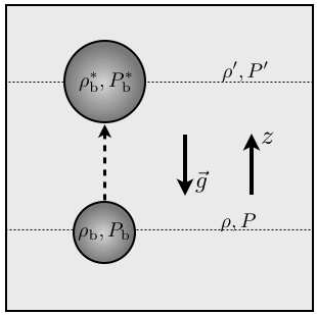
\includegraphics[scale=0.6]{Figures/convection_scheme.png}
    \caption{Σχηματική αναπαράσταση του κριτηρίου Schwarzschild ενάντια στην ύπαρξη ρευμάτων μεταφοράς. Ένα στοιχειώδες κομμάτι αερίου (blob) μετατοπίζεται προς την επιφάνεια του αστέρα όπου διαστέλλεται αδιαβατικά για να διατηρήσει μηχανική ισορροπία με το περιβάλλον του. Αν η πυκνότητα του στοιχειώδους κομματιού είναι μεγαλύτερη από την πυκνότητα του υλικού που το περιβάλλει, θα βυθιστεί πίσω στην αρχική του θέση. Αν όμως η πυκνότητά του είναι μικρότερη από την πυκνότητα του χώρου γύρω του, δυνάμεις άνωσης θα το επιταχύνουν προς τα επάνω και θα δημιουργηθεί ένα ρεύμα μεταφοράς.}
    \label{fig:convection_scheme}
\end{figure}

Αρχικά, το στοιχειώδες κομμάτι αερίου υποθέτουμε ότι βρισκόταν σε κατάσταση μηχανικής και θερμικής ισορροπίας με τον περιβάλλοντα χώρο, ώστε $\rho_b = \rho$ και $P_b = P$. Μετά την μετατόπιση, το κομμάτι πρέπει να επανέλθει σε μία νέα κατάσταση μηχανικής και θερμικής ισορροπίας. Γενικά, ο χρόνος που χρειάζεται για να εδραιώσει μία νέα κατάσταση μηχανικής ισορροπίας είναι ο δυναμικός χρόνος, $\tau_{\text{dyn}}$, ενώ η θερμική ισορροπία επέρχεται πολύ πιο αργά, στον θερμικό χρόνο $\tau_{\text{KH}}$. Επειδή ισχύει ότι $\tau_{\text{dyn}} \ll \tau_{\text{KH}}$, μπορούμε να υποθέσουμε ότι η μηχανική ισορροπία επέρχεται πριν προλάβει να γίνει ανταλλαγή θερμότητας με το περιβάλλον, ώστε η διαδικασία της μετατόπισης να είναι προσεγγιστικά αδιαβατική και να ισχύει $P_b^{\star} = P^{\prime}$ αλλά γενικά $\rho_b^{\star} \neq \rho^{\prime}$. Αυτό σημαίνει ότι η παραπάνω διαδικασία μπορεί να περιγραφεί από μία αδιαβατική καταστατική εξίσωση της μορφής $P \propto \rho^{\gamma}$, όπου $\gamma$ ο αδιαβατικός δείκτης. Έτσι, μπορούμε να γράψουμε

\begin{align*}
    \begin{cases}
        P_b &\propto \rho_b^{\gamma} \\
        P_b^{\star} &\propto {\rho_b^{\star}}^{\gamma}
    \end{cases} &\Rightarrow
    \frac{ P_b^{\star}}{P_b} \propto \left(\frac{\rho_b^{\star}}{\rho_b}\right)^{\gamma} \Rightarrow \rho_b^{\star} \propto \rho_b \left(\frac{P_b^{\star}}{P_b} \right)^{1/\gamma} \Rightarrow \\\\
    &\Rightarrow \rho_b^{\star} \propto \rho_b \left(\frac{P^{\prime}}{P} \right)^{1/\gamma} \xRightarrow{\eqref{eq:convection:pressure_perturbation}}{\rho_b^{\star} = \rho_b \left(1 + \frac{1}{P} \frac{dP}{dr}\delta r \right)^{1/\gamma}}
\end{align*}

Στο όριο των μικρών μετατοπίσεων $\delta r$, μπορούμε να χρησιμοποιήσουμε ανάπτυγμα Taylor για να δείξουμε ότι
\begin{eqnarray}
    \label{eq:convection:new_blob_density_expression}
    \rho_b^{\star} = \rho + \frac{\rho}{\gamma P} \frac{dP}{dr} \delta r
\end{eqnarray}
όπου χρησιμοποίησαμε την αρχική συνθήκη $\rho_b = \rho$, και ότι το ανάπτυγμα Taylor της συνάρτησης $f(x) = (1+x)^{1/\gamma}$ δίνεται προσεγγιστικά από $f(x) \simeq 1 + \frac{1}{\gamma}x + \dots$.

Έστω ένα στρωματοποιημένο (stratified) υλικό στο οποίο $d\rho/dr < 0$ και $dP/dr < 0 $. Σε αυτή την περίπτωση, εαν $\rho_b^{\star} > \rho^{\prime}$ τότε το στοιχειώδες κομμάτι αερίου είναι πιο βαρύ από τον περιβάλλοντα χώρο στον οποίο βρίσκεται και θα βυθιστεί στην αρχική του θέση. Τότε το σύστημα είναι σταθερό ως προς τη δημιουργία ρεύματος μεταφοράς. Αν όμως $\rho_b^{\star} < \rho^{\prime}$, τότε δημιουργείται αστάθεια καθώς δυνάμεις άνωσης θα το επιταχύνουν προς τα επάνω. Από τις σχέσεις \eqref{eq:convection:density_perturbation} και \eqref{eq:convection:new_blob_density_expression} προκύπτει ότι η ευστάθεια απαιτεί
\begin{equation}
    \label{eq:convection:schwarzschild_density_pressure}
    \rho_b^{\star} > \rho^{\prime} \Rightarrow \boxed{\frac{d\rho}{dr} < \frac{\rho}{\gamma P} \frac{dP}{dr}}
\end{equation}
ή ισοδύναμα, διαιρώντας με $dP/dr$ (το οποίο είναι αρνητικό)
\begin{equation}
    \label{eq:convection:schwarzschild_log_density_log_pressure}
    \boxed{\frac{d\log \rho}{d\log P} > \frac{1}{\gamma}}
\end{equation}
Η σχέση \eqref{eq:convection:schwarzschild_log_density_log_pressure} ονομάζεται \textbf{κριτήριο ευστάθειας Schwarzschid}, και αν παραβιαστεί τότε έχουμε την δημιουργία ρευμάτων μεταφοράς.

Παρόλα αυτά, οι σχέσεις \eqref{eq:convection:schwarzschild_density_pressure} και \eqref{eq:convection:schwarzschild_log_density_log_pressure} απαιτούν τον υπολογισμό βαθμίδας πυκνότητας που δεν είναι μέρος των διαφορικών εξισώσεων που περιγράφουν την αστρική δομή. Θα προτιμούσαμε να εκφράσουμε το κριτήριο του Schwarzschild με τη μορφή θερμοβαθμίδας, όπως αυτή εμφανίζεται στην εξίσωση μεταφοράς ενέργειας με ακτινοβολίας (σχέσεις \ref{eq:energy_transport_radiation_eulerian_diff} -- \ref{eq:radiative_temperature_gradient}).
Χρησιμοποιώντας ότι 
\begin{equation*}
    \rho = \rho(P,T) = \frac{\mu m_H}{kT}P
\end{equation*}
μπορούμε να δείξουμε οτι
\begin{align}
    \label{eq:convection:dRho_dr}
    \nonumber \frac{d\rho}{dr} &= \frac{\mu m_H}{k} \left(\frac{1}{T} \frac{dP}{dr} - \frac{P}{T^2}\frac{dT}{dr} \right) = \underbrace{\frac{\mu m_H}{kT}P}_{= \,\rho} \left(\frac{1}{P} \frac{dP}{dr} - \frac{1}{T} \frac{dT}{dr} \right) \Rightarrow \\\nonumber\\
    &\Rightarrow \frac{d\rho}{dr} = \frac{\rho}{P} \frac{dP}{dr} - \frac{\rho}{T} \frac{dT}{dr}
\end{align}
Από τις σχέσεις \eqref{eq:convection:density_perturbation} και \eqref{eq:convection:dRho_dr} προκύπτει ότι
\begin{align*}
    \rho^{\prime} &= \rho + \frac{d\rho}{dr} \delta r = \rho + \left(\frac{\rho}{P} \frac{dP}{dr} - \frac{\rho}{T} \frac{dT}{dr} \right)\delta r \Rightarrow \\\\
    &\Rightarrow \rho^{\prime} - \rho = \left(\frac{\rho}{P} \frac{dP}{dr} - \frac{\rho}{T} \frac{dT}{dr} \right)\delta r \xRightarrow{\eqref{eq:convection:new_blob_density_expression}} \\\\
    &\Rightarrow \rho^{\prime} - \rho_b^{\star} + \frac{\rho}{\gamma P} \frac{dP}{dr} \delta r = \left(\frac{\rho}{P} \frac{dP}{dr} - \frac{\rho}{T} \frac{dT}{dr} \right)\delta r \Rightarrow \\\\
    &\Rightarrow \rho_b^{\star} - \rho^{\prime} = \left(- \frac{\gamma - 1}{\gamma}\frac{\rho}{P} \frac{dP}{dr} + \frac{\rho}{T} \frac{dT}{dr} \right)\delta r
\end{align*}

Η ευστάθεια απαιτεί $\rho_b^{\star} - \rho^{\prime} > 0$, άρα αφού $dP/dr < 0$ και $dT/dr < 0$, θα έχουμε
\begin{align}
    \label{eq:convection:schwarzschild_criterion_dT_dr}
    \nonumber \rho_b^{\star} &- \rho^{\prime} > 0 \Rightarrow \left(- \frac{\gamma - 1}{\gamma}\frac{1}{P} \frac{dP}{dr} + \frac{1}{T} \frac{dT}{dr}\right) \rho \delta r > 0 \xRightarrow{\rho > 0, \delta r > 0} \\\nonumber \\
    \nonumber &\Rightarrow - \frac{\gamma - 1}{\gamma}\frac{1}{P} \frac{dP}{dr} + \frac{1}{T} \frac{dT}{dr} > 0 \Rightarrow \\\nonumber\\
    &\Rightarrow \boxed{\left| \frac{dT}{dr} \right| < \frac{\gamma - 1}{\gamma} \frac{T}{P} \left| \frac{dP}{dr}\right|}
\end{align}
Η τελευταία μορφή του κριτηρίου Schwarzschild μας δείχνει ότι όταν η θερμοβαθμίδα γίνει πολύ μεγάλη, τότε το σύστημα γίνεται ασταθές ως προς την εμφάνιση ρευμάτων μεταφοράς, και μαζί με την σχέση \eqref{eq:energy_transport_radiation_eulerian_diff} για την περίπτωση μεταφοράς ενέργειας με ακτινοβολία, αποτελεί την τέταρτη διαφορική εξίσωση που περιγράφει τη δομή ενός αστέρα (αν αντί για ανισότητα πάρουμε ισότητα), στην περίπτωση που έχουμε μεταφορά ενέργειας μέσω δινορευμάτων.

Παρόλα αυτά, υπάρχει ακόμα ένας τρόπος να γράψουμε το κριτήριο του Schwartzschild και η οποία θα μας επιτρέψει να αντιληφθούμε καλύτερα το πότε η μεταφορά ενέργειας μέσω δινορευμάτων υπερισχύει αυτής της ακτινοβολίας.
Γράφοντας την καταστατική εξίσωση σε διαφορική μορφή (δες Παράρτημα \ref{apx:kinetic_theory}), η διακύμανση της πυκνότητας ως προς την πίεση σε όλον τον αστέρα θα είναι
\begin{align}
    \label{eq:convection:dlogRho_dlogP_actual_temp_gradient}
    \nonumber \frac{dP}{P} &= \chi_\rho \frac{d\rho}{\rho} + \chi_T \frac{dT}{T} \Rightarrow \\\nonumber\\
    \nonumber &\Rightarrow d\log P = \chi_\rho d\log \rho + \chi_T d\log T \Rightarrow \\\nonumber\\
     &\Rightarrow \frac{d\log \rho}{d \log P} = \frac{1}{\chi_\rho} \left( 1 - \chi_T \nabla \right)
\end{align}
όπου χρησιμοποιήσαμε το γεγονός ότι $d\log P = dP/P$, $d\log \rho = d\rho/\rho$ και $d\log T = dT/T$. Η ποσότητα $\displaystyle \nabla = \frac{d\log T}{d \log P}$ ονομάζεται \textbf{πραγματική θερμοβαθμίδα} (actual temperature gradient).

Για μια αδιαβατική μεταβολή ($dT = 0$), ισχύει 
\begin{equation}
    \frac{dP}{P} = \underbrace{\chi_\rho}_{= \,\gamma} \frac{d\rho}{\rho} + \chi_T \frac{\cancelto{0}{dT}}{T} \Rightarrow \frac{dP}{P} = \gamma \frac{d\rho}{\rho} \Rightarrow \frac{d\log P}{d\log \rho} = \gamma 
\end{equation}
και άρα συνδυάζοντας το παραπάνω αποτέλεσμα με τη σχέση \eqref{eq:convection:dlogRho_dlogP_actual_temp_gradient}, μπορούμε να γράψουμε για το στοιχειώδες κομμάτι αερίου που μετατοπίστηκε ότι
\begin{equation}
    \label{eq:convection:nabla_ad}
    \frac{1}{\gamma} = \frac{1}{\chi_\rho} \left(1 - \chi_T \nabla_{\text{ad}} \right) \Rightarrow \nabla_{\text{ad}} = \frac{\gamma - \chi_\rho}{\gamma \chi_T}
\end{equation}
όπου η ποσότητα $\displaystyle \nabla_{\text{ad}} = \left(\frac{\partial \log T}{\partial \log P} \right)_{\text{ad}}$ είναι η \textbf{αδιαβατική θερμοβαθμίδα}. Επειδή για το ιδανικό αέριο ισχύει $\chi_{\rho} = \chi_T = 1$, έχουμε ότι
\begin{equation}
    \nabla_{\text{ad}} = \frac{\gamma - 1}{\gamma}
\end{equation}

Συνδυάζοντας όλα τα παραπάνω, η έκφραση του κριτηρίου Schwartzschild \eqref{eq:convection:schwarzschild_log_density_log_pressure} γράφεται
\begin{align}
    \label{eq:convection:schwartzscild_criterion_actual_temp_gradient}
    \nonumber \frac{d\log \rho}{d\log P} &> \frac{1}{\gamma} \Rightarrow \frac{1}{\chi_\rho} \left( 1 - \chi_T \nabla \right) > \frac{1}{\chi_\rho} \left(1 - \chi_T \nabla_{\text{ad}} \right) \\\nonumber\\
    \nonumber &\Rightarrow 1 - \chi_T \nabla > 1 - \chi_T \nabla_{\text{ad}} \Rightarrow \chi_T \nabla < \chi_T \nabla_{\text{ad}} \Rightarrow \\\nonumber\\
    &\Rightarrow \boxed{\nabla < \nabla_{\text{ad}}}
\end{align}

Αν όλη η ενέργεια μεταφέρεται μέσω ακτινοβολίας, τότε $\nabla = \nabla_{\text{rad}}$, όπως δίνεται από την σχέση \eqref{eq:radiative_temperature_gradient} και άρα καταλήγουμε στο ότι
\begin{equation}
    \label{eq:convection:schwarzschild_criterion_nabla_rad_nabla_ad}
    \boxed{\nabla_{\text{rad}} < \nabla_{\text{ad}}}
\end{equation}
Σημασία πρέπει να δοθεί στα διάφορα $\nabla$ σύμβολα που εμφανίζονται στις διάφορες μορφές του κριτηρίου Schwarzschild. Το $\nabla_{\text{rad}}$ παριστάνει την \textit{χωρική θερμοβαθμίδα}, ενώ το $\nabla_{\text{ad}}$ παριστάνει την μεταβολή της θερμοκρασίας σε ένα στοιχειώδες κομμάτι αερίου που υπόκειται σε μια μεταβολή πίεσης.

Σύμφωνα λοιπόν με το κριτήριο Schwarzschild, περιμένουμε να έχουμε μεταφορά ενέργειας μέσω δινορευμάτων εαν
\begin{equation*}
    \nabla_{\text{rad}} = \frac{3}{16\pi \alpha c G} \frac{\kappa l P}{m T^4} > \nabla_{\text{ad}}
\end{equation*}
Αυτό προϋποθέτει ένα από τα ακόλουθα
\begin{itemize}
    \item Μία μεγάλη τιμή του $\kappa$, δηλαδή έχουμε ρεύματα μεταφοράς σε περιοχές όπου η αδιαφάνεια είναι μεγάλη. Παραδείγματα τέτοιων περιοχών είναι τα εξωτερικά στρώματα του Ήλιου και άλλων ψυχρών αστέρων, καθώς η αδιαφάνεια αυξάνεται όσο μειώνεται η θερμοκρασία (δες αδιαφάνεια κατά Kramer). Αφού αστέρες χαμηλής μάζας (μεταγενέστερου φασματικού τύπου) είναι πιο ψυχροί από αστέρες μεγάλης μάζας (προγενέστερου φασματικού τύπου), περιμένουμε αστέρες χαμηλής μάζας να έχουν εξωτερικά στρώματα που εμφανίζουν δινορεύματα.
    
    \item Μία μεγάλη τιμή του $l/m$, δηλαδή περιοχές με μεγάλη ροή ενέργειας. Σύμφωνα με τη σχέση \eqref{eq:thermal_equilibrium_lagrangian_form}, προς τον πυρήνα έχουμε $l/m \approx E_{\text{nuc}}$, έτσι αστέρες που έχουν παραγωγή ενέργειας στο κέντρο τους αναμένεται να έχουν πυρήνες που εμφανίζουν δινορεύματα. Αυτό συμβαίνει σε αστέρες σχετικά μεγάλης μάζας. 
    
    \item Μία μικρή τιμή του $\nabla_{\text{ad}}$, κάτι που συμβαίνει σε περιοχές μερικού ιονισμού σε σχετικά χαμηλές θερμοκρασίες (partial ionization zones). Έτσι, ακόμα κι αν η αδιαφάνεια δεν είναι πολύ μεγάλη, τα στρώματα της επιφάνειας ενός αστέρα μπορεί να είναι ασταθή όσον αφορά την δημιουργία δινορευμάτων. Αποδεικνύεται ότι αστέρες ανεξαρτήτου μάζας έχουν ρηχές επιφανειακές περιοχές στις οποίες εμφανίζονται δινορεύματα, σε θερμοκρασίες όπου το υδρογόνο και το ήλιο είναι μερικώς ιονισμένα. 
\end{itemize}

Τέλος, πρέπει να αναφέρουμε ότι δεν είναι καθόλου εύκολο να αναπτύξουμε μία αναλυτική θεωρία για τα ρεύματα μεταφοράς και ότι αποτελεί ένα πολύ ενεργό πεδίο έρευνας της Αστροφυσικής. Προκειμένου να έχουμε μία εκτίμηση για το πόση ενέργεια μπορεί να μεταφερθεί μέσω των δινορευμάτων, καταφεύγουμε σε μία απλή μονοδιάστατη "θεωρία" που βασίζεται σε πολλές προσεγγίσεις και είναι γνωστή ως "mixing length theory" (MLT)\footnote{Συχνά η MLT προσεγγίζεται ως μία διαδικασία διάχυσης.}. Σύμφωνα με αυτή, το στοιχειώδες κομμάτι αερίου ταξιδεύει μία χαρακτηριστική απόσταση $\ell_m$ (το mixing length) πάνω ή κάτω, μετά το πέρας της οποίας το κομμάτι αερίου έχει υιοθετήσει τα χαρακτηριστικά του μέσου που το περιβάλλει. Το χαρακτηριστικό αυτό μήκος είναι της τάξης του τοπικού pressure scale height, $H_P$, ($\ell_m \sim H_P$) όπου είναι η ακτινική απόσταση κατά την οποία η πίεση αλλάζει κατά έναν παράγοντα $e$.

\begin{equation}
    H_P = \left|\frac{dr}{d\ln P} \right| = \frac{P}{\rho g}
\end{equation}
Η τελευταία ισότητα ισχύει στην περίπτωση που ο αστέρας βρίσκεται σε κατάσταση υδροστατικής ισορροπίας. Η ροή των δινορευμάτων αποδεικνύεται ότι συνδέεται με την υπεραδιαβατικότητα (superadiabaticity), $\nabla - \nabla_{\text{ad}}$, η οποία δείχνει τον βαθμό στον οποίο η πραγματική θερμοβαθμίδα $\nabla$, ξεπερνάει την αδιαβατική τιμή

\begin{equation}
    F_{\text{conv}} = \rho \,c_P T \left( \frac{\ell_m}{H_P} \right)^2 \sqrt{\frac{1}{2} g H_P} \left(\nabla - \nabla_{\text{ad}} \right)^{3/2}
\end{equation}

Όσο προσεγγίζουμε την επιφάνεια του αστέρα, τα δινορεύματα γίνονται πολύ αναποτελεσματικά στην μεταφορά ενέργειας. Τότε $F_{\text{conv}} \ll F_{\text{rad}}$ ώστε η ακτινοβολία να μεταφέρει πρακτικά όλη την ενέργεια, και $\nabla \approx \nabla_{\text{rad}}$ παρά την παρουσία δινορευμάτων.
%% ---------------------------------------------------------------------------------------------------- %%
%% ---------------------------------------------------------------------------------------------------- %%
%% ---------------------------------------------------------------------------------------------------- %%
\subsubsection{Σύνοψη εξισώσεων αστρικής δομής}
\begin{itemize}
    \item Εξίσωση συνέχειας
    
    \begin{equation*}
        \frac{dm}{dr} = 4\pi r^2 \, \rho(r)
    \end{equation*}
    
    \item Εξίσωση υδροστατικής ισορροπίας
    
    \begin{equation*}
        \frac{dP}{dr} = - G \frac{m(r) \,\rho(r)}{r^2}
    \end{equation*}
    
    \item Εξίσωση θερμικής ισορροπίας
    
    \begin{equation*}
        \frac{dl}{dr} = 4\pi r^2 \,\rho(r) \left(\epsilon_{\text{nuc}} - \epsilon_\nu - T \frac{ds}{dt} \right)
    \end{equation*}
    
    \item Εξίσωση διάδοσης ενέργειας
    Γενικά, η στρωματοποίηση της θερμοκρασίας (temperature stratification) μπορεί να περιγραφεί από 
    \begin{align*}
        \nabla &= \frac{\partial \ln \,T}{\partial \ln \,P} = \frac{P}{T} \frac{\partial T}{\partial P} = \frac{P}{T} \frac{\partial T}{\partial r} \frac{\partial r}{\partial P}  \Rightarrow \\\\
        & \Rightarrow \frac{\partial T}{\partial r} = \nabla \frac{T}{P} \frac{\partial P}{\partial r} \Rightarrow \boxed{\frac{\partial T}{\partial r} = \nabla \frac{T}{P} \frac{Gm \rho}{r^2}}
    \end{align*}
    
    Αν η ενέργεια μεταφέρεται με ακτινοβολία ($\nabla = \nabla_{\text{rad}}$):
    \begin{equation*}
        \frac{dT}{dr} = - \frac{3 \,\kappa(r) \,\rho(r) \,l}{16 \,\pi \,\alpha \,c \,r^2 \,T^3}
    \end{equation*}
    
    Αν η ενέργεια μεταφέρεται με ρεύματα μεταφοράς ($\nabla = \nabla_{\text{ad}}$):
    \begin{equation*}
        \frac{dT}{dr} = \frac{\gamma - 1}{\gamma} \frac{T}{P} \frac{dP}{dr} = - \frac{\gamma - 1}{\gamma} \frac{G \,m(r) \,\rho(r)}{r^2} \frac{T}{P}
    \end{equation*}
    
    Σε κάθε φλοιό πρέπει να ελέγχουμε αν $\nabla_{\text{rad}} < \nabla_{\text{ad}}$, στην οποία περίπτωση πρέπει να χρησιμοποιηθεί η εξίσωση που περιγράφει την μεταφορά ενέργειας με ακτινοβολία αλλιώς πρέπει να χρησιμοποιήθει η εξίσωση μεταφοράς ενέργειας με δινορεύματα. Σε περιοχές χαμηλής πυκνότητας πρέπει να υπολογίζουμε το $\nabla_{\text{conv}}$ χρησιμοποιώντας τη θεωρία των ρευμάτων μεραφοράς.
\end{itemize}

Οι παραπάνω εξισώσεις πρέπει να συνοδεύονται από συμπληρωματικές σχέσεις, όπως η καταστική εξίσωση $P(\rho, T)$, η αδιαφάνεια $\kappa(\rho, T)$, και ο ρυθμός παραγωγής ενέργειας $\epsilon(\rho, T, X_i)$, καθώς και τέσσερις συνοριακές συνθήκες (δύο στην επιφάνεια: $L = 4\,\pi \,R^2 \,\sigma \,T_{\text{eff}}^4$ και $P=\frac{2GM}{3 R^2 \kappa}$, και δύο στο κέντρο: $M(r) = 0$ και $L(r) = 0$) ώστε να έχουμε συνολικά εφτά εξισώσεις για εφτά άγνωστες μεταβλητές ($P, \,\rho, \,T, \,m(r), \,L(r), \,\kappa, \,\epsilon$) ως συναρτήσεις της ανεξάρτητης μεταβλητής $r$ (ή της $m$ αν επιλέξουμε να εκφράσουμε τις παραπάνω σχέσεις στο σύστημα συντεταγμένων του Lagrange).
%% ---------------------------------------------------------------------------------------------------- %%
%% ---------------------------------------------------------------------------------------------------- %%
%% ---------------------------------------------------------------------------------------------------- %%
\section{Εξέλιξη αστέρων}
Ο κόσμος γύρω μας, καθώς και εμείς οι ίδιοι είμαστε φτιαγμένοι από πάνω από εκατό διαφορετικά χημικά στοιχεία. Σήμερα γνωρίζουμε ότι ζούμε σε ένα σύμπαν πλούσιο σε χημικά στοιχεία που απαρτίζουν όλες τις γνωστές κοσμικές δομές που μπορούμε να παρατηρήσουμε. Έχουμε εντοπίσει περισσότερα από 118 τέτοια στοιχεία, τα οποία από τον 19ο αιώνα κιόλας, είναι κομψά ταξινομημένα σε γραμμές και σε στήλες του περιοδικού πίνακα από τον Dmitri Mendeleev. Από αυτά όμως, λίγα είναι σε αφθονία, όπως το υδρογόνο, ο άνθρακας, το πυρίτιο και ο σίδηρος. Άλλα στοιχεία πάλι, όπως ο χρυσός και το ουράνιο είναι σπάνια και για αυτό η αξία τους είναι μεγάλη και άλλα είναι τεχνητά κι έχουν δημιουργηθεί αποκλειστικά σε εργαστήρια. Ωστόσο, το 99\% της συνηθισμένης βαρυονικής ύλης του σύμπαντος αποτελείται από δύο μόνο στοιχεία: το υδρογόνο και το ήλιο. Για το υδρογόνο, όλες οι ενδείξεις καταδεικνύουν ότι δημιουργήθηκε κατά τις πρώτες στιγμές του σύμπαντος. Το ήλιο ακολούθησε μεταγενέστερα, μέσα στα πρώτα λεπτά μετά την Μεγάλη Έκρηξη.
Για τα υπόλοιπα στοιχεία όμως η διαδικασία της δημιουργίας τους διαφέρει. Για πολλά χρόνια η εξήγηση της προέλευσης των βαρύτερων χημικών στοιχείων ήταν μια μεγάλη πρόκληση για την επιστημονική κοινότητα, όπως και το να εξηγήσουν την αναλογία τους. Στην αρχή αυτής της αναζήτησης, πριν την ανάπτυξη της πυρηνικής φυσικής και της κβαντικής θεωρίας, κανένας δεν γνώριζε την προέλευση τους. Όμως, από τις αρχές της δεκαετίας του 1940 γνωρίζουμε πλέον ότι σημαντικό ρόλο στη δημιουργία των χημικών στοιχείων παίζει η δημιουργία, η εξέλιξη και ο θάνατος των άστρων.  
%% ---------------------------------------------------------------------------------------------------- %%
%% ---------------------------------------------------------------------------------------------------- %%
%% ---------------------------------------------------------------------------------------------------- %%
\subsection{Αφθονία Χημικών Στοιχείων στο Σύμπαν}
Πριν ξεκινήσουμε τη μελέτη μας σχετικά με την δημιουργία των βαρέων στοιχείων στο σύμπαν αξίζει να κοιτάξουμε την κατανομή των χημικών στοιχείων σε αυτό όπως τη βλέπουμε σήμερα. Η συλλογή αυτών των πληροφοριών γίνεται με διάφορους τρόπους όπως μέσα από φασματοσκοπικές παρατηρήσεις, ανάλυση της σύστασης μετεωριτών κ.α. και εκφράζεται από την \textbf{αφθονία} των χημικών στοιχείων στο σύμπαν. Με τον όρο αφθονία ενός στοιχείου ορίζουμε το πόσο συχνά εμφανίζεται ένα στοιχείο σε δεδομένο περιβάλλον σε σύγκριση με τα υπόλοιπα. Για να υπολογίσουμε όμως με ακρίβεια αυτή την αναλογία συνήθως χρησιμοποιούμε ως βάση μας το λόγο μάζας (mass fraction) ή τα ποσοστιαία mole αυτού του στοιχείου, δηλαδή τον λόγο της μάζας του ή τα mole του στοιχείου που θέλουμε να μελετήσουμε ως προς τη συνολική μάζα/mole του ρευστού. Αποφεύγουμε να χρησιμοποιήσουμε τον όγκο, γιατί ειδικά σε μορφές ρευστών όπως τα αέρια και το πλάσμα η συστολή - διαστολή του όγκου τους είναι συχνό φαινόμενο. Η σχετική μάζα για το μίγμα του κοσμικού ρευστού, όπως γνωρίζουμε από την Χημεία ορίζεται ως

\begin{equation}
X_{i}=\frac{m_{i}}{m_{\text{tot}}}
\end{equation}
όπου το σύνολο των σχετικών μαζών του κοσμικού ρευστού είναι:

\begin{equation}
\sum\limits_{i=1}^N m_{i} = m_{\text{tot}} \Rightarrow \sum\limits_{i=1}^N X_{i} =1
\end{equation}
Μια ποσότητα που δεν εκφράζει την συνολική μάζα αλλά την την αριθμητική πυκνότητα ενός πυρήνα είναι η αναλογία:

\begin{equation}
Y_{i}= \frac{X_{i}}{A_{i}}
\end{equation}
όπου $X_i$ ο αριθμός των πρωτονίων ή των νετρονίων και $A_{i}$ o μαζικός αριθμός του πυρήνα. Αν η πυκνότητα μάζας ενός πυρήνα $\rho X_{i}$ διαιρεθεί με τη μάζα ενός πυρήνα $A_{i} m_{u}$, η οποία περιέχει την αριθμητική πυκνότητα:

\begin{equation}
n_{i}= \frac{\rho}X_{i}{A_{i}m_{u}}= \frac{\rho Y_{i}}{m_{u}}=\rho N_{A} Y_{i}
\end{equation}
όπου $N_{A}$ ο αριθμός Avogadro και γνωρίζουμε ότι ισχύει: $N_{A}= 1/ m_{u}$ και $X_{i}$ . Η συνολική αφθονία ηλεκτρονίων (electron-fraction) εκφράζεται ακριβώς όπως εκείνη των ελεύθερων πρωτονίων σε σχέση με τους πυρήνες και είναι της μορφής:

\begin{equation}
Y_{e} = \sum\nolimits_{i} Z_{i} Y_{i}
\end{equation}
όπου $Z_{i}$ το φορτίο του σωματίου. Ο λόγος των ηλεκτρονίων ανά νουκλεόνιο στην ύλη είναι καθοριστικός παράγοντας σε πολλές αστροφυσικές και πυρηνικές μελέτες. Η τιμή αυτού του λόγου μεταβάλλεται όταν ένα πρωτόνιο "αιχμαλωτίζει" ένα ηλεκτρόνιο για τον σχηματισμό ενός νετρονίου.
Ισοδύναμα, έχουμε και τον συνολικό λόγο πρωτονίων ανά νουκλεόνιο:

\begin{equation}
\frac{\sum\nolimits_{i} Z_{i} Y_{i}}{ \sum\nolimits_{i} Y_{i}(Z_{i}+N_{i})}=\frac{\sum\nolimits_{i} Z_{i} Y_{i}}{ \sum\nolimits_{i} A_{i} Y_{i}}= \frac{\sum\nolimits_{i} Z_{i} Y_{i}}{\sum\nolimits_{i} X_{i}}
\end{equation}

Οι αλλαγές στην αφθονία ($\dot{Y_{i}}$) μπορούν να εκφραστούν από μια διαφορική εξίσωση για κάθε πυρηνική αναλογία $Y_{i}$, που θα εκφράζει τις διασπάσεις, πυρηνικές συντήξεις και αντιδράσεις. Σε γενικές γραμμές, η διαφορική εξίσωση που μας δείχνει την αλλαγή στη χημική σύσταση ενός αστέρα μπορεί να γραφτεί ως
\begin{eqnarray}
    \label{eq:composition_differential_equation}
    \boxed{\frac{\partial X_i}{\partial t} = \frac{m_i}{\rho} \left(\sum_j r_{ji} - \sum_k r_{ik} \right), \,i=1,\dots,n}
\end{eqnarray}
όπου $X_i$ είναι ο λόγος μάζας (mass fraction) όλων των ατομικών πυρήνων που παίρνουν μέρος στην διαδικασία της πυρηνοσύνθεσης ($i = 1,\dots,n$), με μάζα $m_i$. Αυτό το σύνολο διαφορικών εξισώσεων περιγράφει την εξέλιξη του αστέρα σε όρους χημικής σύστασης και έρχεται να συμπληρώσει τις τέσσερις γνωστές διαφορικές εξισώσεις που περιγράφουν την δομή του αστέρα.

Η σχετική αφθονία κάθε στοιχείου στο σύμπαν, όπως προκύπτει από τις σημερινές παρατηρήσεις, φαίνεται στο ραβδόγραμμα του σχήματος \ref{fig:abundace_of_elements}.

\begin{figure}
    \centering
    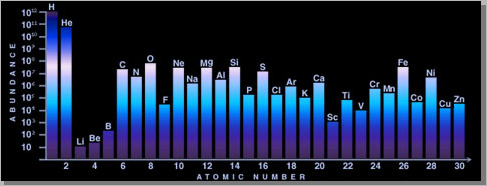
\includegraphics[scale=0.75]{Figures/atomic1.jpg} 
    \caption{Η αφθονία των χημικών στοιχείων στο σύμπαν.}  
    \label{fig:abundace_of_elements}
\end{figure}

Το αποτύπωμα της κοσμικής πυρηνοσύνθεσης βαρέων στοιχείων βρίσκεται και μέσα στην αφθονία των στοιχείων του ηλιακού συστήματος (σχήμα \ref{fig:solar_abundance_of_elements}). Η ηλιακή φωτόσφαιρα και οι μετεωρίτες αντικατοπτρίζουν την χημική υπογραφή του νέφους μέσα από το οποίο γεννήθηκε ο ήλιος. Αυτή η αφθονία όμως, φαίνεται να εκφράζει την γενικότερη συμπεριφορά της δημιουργίας των πυρήνων στο σύμπαν. Αξίζει να παρατηρήσουμε τις κορυφές στα στοιχεία με ατομικούς αριθμούς $A =$ 80, 130 και 195 --οι οποίοι αντιστοιχούν σε μαγικούς αριθμούς-- καθώς η σύνθεση αυτών των στοιχείων προέρχεται αποκλειστικά μέσω των διεργασιών που αναλύουμε στο παράρτημα \ref{apx:nucleosynthesis}.

\begin{figure}
    \centering
    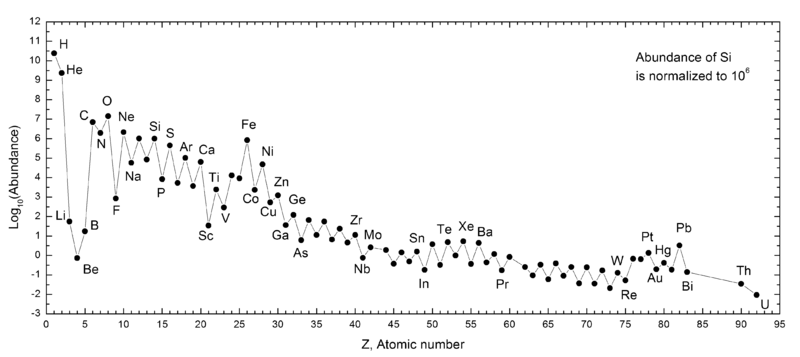
\includegraphics[scale=0.45]{Figures/SolarSystemAbundances.png} 
    \caption{Η αφθονία των χημικών στοιχείων στο ηλιακό μας σύστημα.}
    \label{fig:solar_abundance_of_elements}
\end{figure}

Σχεδόν όλη μάζα των στοιχείων συγκεντρώνεται στα στοιχεία του υδρογόνου και του ηλίου, τα οποία φαίνεται να παρήχθησαν κατά τη γέννηση του σύμπαντος. Η επικράτηση των πυρήνων μικρού ατομικού αριθμού $A$ έναντι των μεγαλυτέρων δεν είναι τυχαία και φαίνεται να οφείλεται σε δυο παράγοντες. Ο ένας παράγοντας είναι ότι σε μεγαλύτερους πυρήνες, η διαδικασία της σύντηξης απαιτεί μεγαλύτερη ενέργεια έτσι ώστε να ξεπεραστεί το απωστικό δυναμικό Coulomb καθώς η πιθανότητα μιας τέτοιας σύντηξης παρουσιάζει εκθετική εξάρτηση του προϊόντος από τα φορτισμένα αντιδρώντα. Για παράδειγμα, η σύντηξη δυο πυρήνων οξυγόνου θα  μας δώσει έναν πυρήνα 64 φορές μεγαλύτερο από εκείνον που θα μας δώσει η σύντηξη δυο πυρήνων υδρογόνου. Ο άλλος παράγοντας φαίνεται να είναι ο αριθμός των νουκλεονίων του πυρήνα. Όπως έχουμε δει και στα παραπάνω διαγράμματα, ο επόμενος εμφανιζόμενος πυρήνας με μονό αριθμό νουκλεονίων μετά το $^{1}$H είναι το $^{25}$Mg που είναι πολύ χαμηλός σε ποσοστά εμφάνισης. Με μια προσεκτικότερη ματιά στις χημικές αναλογίες είναι προφανές ότι υπάρχει μια προτίμηση στη δημιουργία πυρήνων με ζυγό αριθμό νουκλεονίων έναντι σε εκείνους με μονό αριθμό. Επίσης, φαίνεται να υπάρχει σαφής προτίμηση δημιουργίας πυρήνων που έχουν ζυγό-ζυγό αριθμό νουκλεονίων. Για παράδειγμα, στα πρώτα 25 στοιχεία μόνο το $^{14}$N δεν είναι ζυγός-ζυγός πυρήνας, δηλαδή δεν έχει ζυγό αριθμό πρωτονίων και ζυγό αριθμό νετρονίων. Επιπλέον εκτός από τον $^{56}$Fe όλοι οι υπόλοιποι συχνά εμφανιζόμενοι πυρήνες έχουν ζυγούς- ζυγούς πυρήνες αλλά και $Z=N$. Τους πυρήνες με αυτή την ιδιότητα τους ονομάζουμε \textbf{alpha-particle nuclei} εξαιτίας της ομοιότητάς του με τον πρώτο εμφανιζόμενο ζυγό-ζυγό πυρήνα, τον πυρήνα του $^{4}$He. Αυτό εξηγείται μέσω του πυρηνικού μοντέλου φλοιών, δηλαδή στο ότι οι ατομικοί πυρήνες αυξάνουν τις διαστάσεις τους σχηματίζοντας κελύφη γεμάτα με πρωτόνια και νετρόνια. Μόνο συγκεκριμένοι συνδυασμοί αριθμών πρωτονίων και νετρονίων φαίνεται να εμφανίζουν τους ισχυρότερους δεσμούς σύνδεσης και άρα ευσταθή στοιχεία. Τους συνδυασμούς αυτούς τους ονομάζουμε \textbf{μαγικούς αριθμούς}. Πλέον είναι προφανές ότι τα στοιχεία σε μεγαλύτερη αφθονία είναι εκείνα που έχουν διπλά μαγικούς όπως τα: $^{4}$He με $Z = N = 2$, $^{16}$O με $Z = N = 8$, $^{40}$Ca με $Z = N = 20$ και ακόμα και για τον σίδηρο $^{56}$Fe φαίνεται ότι αρχικά δημιουργήθηκε ως τον alpha-particle πυρήνα $^{56}$Ni με $Z = N = 28$. Μετά όμως από τη δημιουργία αυτού του στοιχείου, η διαδιακασία δημιουργίας βαρύτερων στοιχείων φαίνεται να αλλλάζει χαρακτήρα και να προέρχεται από μια διαφορετική διαδιακασία από εκείνη της σύντηξης. Την διαδικασία αυτή θα την αναλύσουμε εκτενώς παρακάτω και δεν είναι άλλη από εκείνη της αρπαγής νετρονίων. Τέλος, στο παρακάτω διάγραμμα Segre (σχήμα \ref{fig:segre_diagram}) φαίνεται μια ολοκληρωμένη εικόνα της τελικής εξέλιξης της πυρηνοσύνθεσης.

\begin{figure}
    \centering
    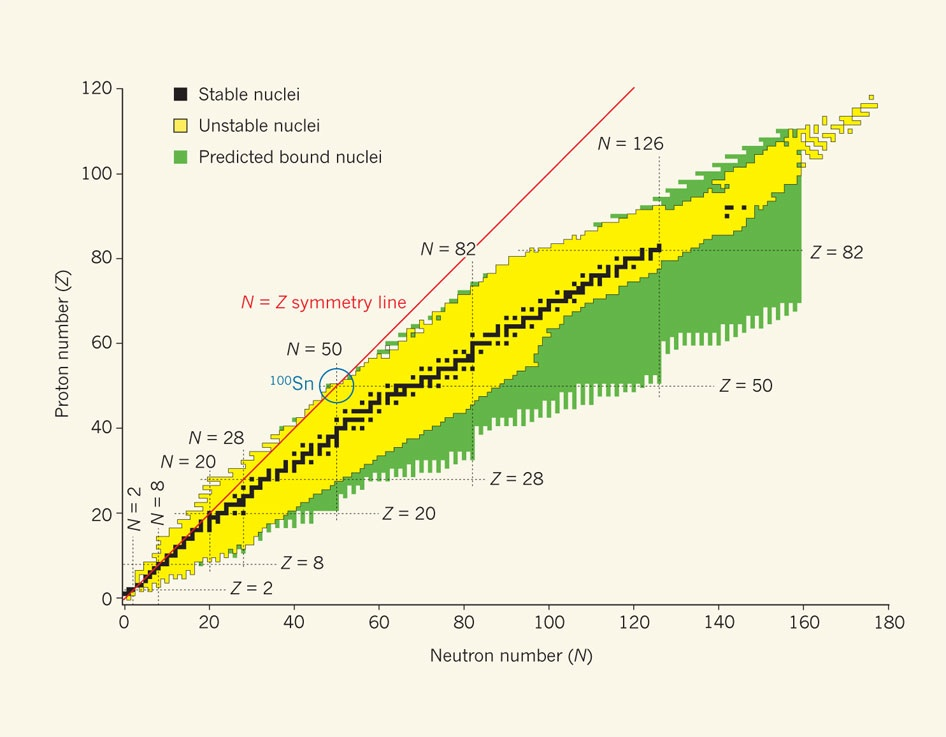
\includegraphics[scale=0.3]{Figures/Nuclei-as-function-of-N-Z.jpg} 
     \caption{Διάγραμμα Segre. Τα στοιχεία που εμφανίζονται με μαύρες κουκκίδες είναι σταθερά ισότοπα και αποτελούν την κοιλάδα σταθερότητας.} 
     \label{fig:segre_diagram}
\end{figure}
%% ---------------------------------------------------------------------------------------------------- %%
%% ---------------------------------------------------------------------------------------------------- %%
%% ---------------------------------------------------------------------------------------------------- %%
\subsection{Δημιουργία πρωτοαστέρων}
Τα άστρα δημιουργούνται κατά κανόνα από τη μεσοαστρική ύλη που υπάρχει στους γαλαξίες και η οποία αποτελείται κυρίως από υδρογόνο, ήλιο, και μοριακή σκόνη. Η ύλη αυτή, όπως και στο αρχέγονο σύμπαν, συχνά σχηματίζει νέφη τεραστίων διαστάσεων και χαμηλής πυκνότητας, τα νεφελώματα. Αυτά τα νέφη εξαιτίας της μεγάλης μάζας τους έχουν και την αντίστοιχη βαρυτική δυναμική ενέργεια, η οποία όμως λόγω της χαμηλής τους πυκνότητας, δεν είναι ικανή να υπερνικήσει τις θερμικές κινήσεις των μορίων και να προκαλέσει τη βαρυτική συστολή και συμπύκνωση.
Ο Jeans έδειξε ότι η δύναμη της πίεσης παύει να αντισταθμίζει τη βαρυτική έλξη, όταν οι διαστάσεις του νέφους είναι μεγαλύτερες, σε τάξη μεγέθους, από το \textbf{μήκος Jeans} που δίνεται απο τη σχέση
\begin{eqnarray}
    \label{eq:jeans_length}
    L_{\text{J}} = \left(\frac{14}{4\pi} \right)^{1/2} \left(\frac{kT}{\mu m_{\text{H}} G \rho} \right)^{1/2}
\end{eqnarray}
Στην περίπτωση αυτή όλη η ύλη, $M_{\text{J}}$, που περιέχεται σε μία σφαίρα με ακτίνα $L_{\text{J}}$, η οποία ισούται με
\begin{equation}
    \label{eq:jeans_mass}
    M_{\text{J}} = \frac{4}{3} \pi \rho L_{\text{J}} = \left(\frac{3}{4\pi \rho} \right)^{1/2} \left( \frac{5kT}{\mu m_{\text{H}} G} \right)^{3/2}
\end{equation}
συμπυκνώνεται και δημιουργεί ένα αστρικό αντικείμενο. Συμπερασματικά, η συμπύκνωση ευνοείται όταν η θερμοκρασία είναι μικρή, και η πυκνότητα μεγάλη. Ανάλογα με το μέγεθος της μάζας (το οποίο εξαρτάται από τη θερμοκρασία, την πυκνότητα και το μέσο μοριακό βάρος του αερίου), το αντικείμενο αυτό μπορεί να είναι ένας αστέρας, ένα σμήνος αστέρων ή και ένας γαλαξίας.

Για να εγκαταλείψει το νεφος την ισορροπία και να αρχίσει η συστολή απαιτείται μια αρχική διαταραχή, μήκους κύματος μεγαλύτερου ή ίσου με το χαρακτηριστικό μήκος Jeans γι' αυτό το νέφος. Διάφοροι παράγοντες μπορεί να επιφέρουν την βαρυτική κατάρρευση, μερικοί από τους οποίους είναι
  
  \begin{itemize}
  \item \textbf{Σύγκρουση Νεφών}\\
  Κατά τη σύγκρουση δυο ή περισσοτέρων νεφών η πυκνότητά τους αυξάνεται τοπικά δημιουργώντας έτσι περιοχές αστρογέννησης.
  
  \item \textbf{Έκρηξη Υπερκαινοφανούς Αστέρα (supernova)}\\
Όπως θα αναφέρουμε και παρακάτω, το τέλος ενός αστέρα μεγάλης μάζας συνοδεύται από την έκρηξή του. Σε μία τέτοια έκρηξη, το μεγαλύτερο μέρος ενός αστεριού (ή και ολόκληρο το αστέρι) διαλύεται και η ύλη του εκσφενδονίζεται βίαια στο διάστημα. Το ωστικό κύμα αυτής της έκρηξης συμπιέζει τα γειτονικά νέφη και δίνει το έναυσμα για τη βαρυτική συστολή.

  \item \textbf{Ύπαρξη νεαρών αστέρων μεγάλης μάζας}\\
 Όταν στην περιοχή των νεφών έχουν ήδη σχηματισθεί νέα μεγάλα αστέρια, αυτά εκπέμπουν τεράστια ποσά ακτινοβολίας η πίεση της οποίας επιδρά πάνω στην ύλη των γειτονικών νεφών και κάτω από τις κατάλληλες συνθήκες μπορεί να επιφέρει βαρυτική κατάρρευση.
 
 \item \textbf{Σπειροειδή Κύματα Πυκνότητας}\\
Σύμφωνα με τη θεωρία κυμάτων πυκνότητας (Lin και Shu, 1963), σπειροειδή κύματα πυκνότητας ξεκινούν από τον πυρήνα του γαλαξία και ξετυλίγονται προς τα έξω στον γαλαξιακό δίσκο. Τα κύματα αυτά συμπιέζουν το αέριο του δίσκου στα σημεία διεύλευσής τους προκαλώντας τη βαρυτική συστολή των μεσοαστρικών νεφών και τη δημιουργία νέων άστρων. Σε κάθε περίπτωση η παρουσία της πίεσης είναι απαραίτητη για να υπερνικηθούν οι τυχαίες θερμικές κινήσεις των μορίων.
\end{itemize}

Αυτή η βαρυτική κατάρρευση έχει ως επακόλουθο την εξώθερμη σύντηξη του υδρογόνου. Από τη στιγμή που σε ένα αστέρι ξεκινήσουν οι  θερμοπυρηνικές αντιδράσεις στον πυρήνα του, αρχίζει να ακτινοβολεί έντονα και ξεκινάει τη "ζωή" του. Αστέρια με μεγάλη μάζα έχουν μεγάλη βαρύτητα, συνεπώς μεγάλη πίεση και θερμοκρασία στον πυρήνα τους. Έτσι, οι συγκρούσεις μεταξύ των πυρήνων υδρογόνου είναι συχνότερες με αποτέλεσμα ο ρυθμός μεταστοιχείωσης του υδρογόνου να είναι μεγάλος. Επομένως, η παραγωγή και η ακτινοβολία ενέργειας είναι επίσης μεγάλες, έτσι ώστε τα αστέρια με μεγάλη μάζα να έχουν μεγάλη επιφανειακή θερμοκρασία και λαμπρότητα. Αντιθέτως, αστέρια με μικρή μάζα ακτινοβολούν λιγότερο. Οι μάζες των αστεριών ποικίλουν αλλά εντός συγκεκριμένων ορίων ($0.08 M_{\odot}<M<150 M_{\odot}$).
%% ---------------------------------------------------------------------------------------------------- %%
%% ---------------------------------------------------------------------------------------------------- %%
%% ---------------------------------------------------------------------------------------------------- %%
\subsubsection{Γραμμή Hayashi}
Η γενικά παραδεκτή σήμερα θεωρία εξέλιξης των πρωτοαστέρων είναι αυτή που πρότεινε ο Ιάπωνας αστρονόμος Hayashi. Στην αρχή το μεσοαστρικό νέφος που συστέλελται είναι οπτικά διαφανές (οπτικό βάθος $\tau \ll 1$) επειδή η πυκνότητά του είναι μικρή. Έτσι η ενέργεια που παράγεται στο εσωτερικό του, λόγω της βαρυτικής συστολής, ακτινοβολείται ελεύθερα στο μεσοαστρικό χώρο. Κατά τη διάρκεια αυτής της φάσης η θερμοκρασία στο εσωτερικό του νέφους παραμένει σταθερή και ίση με την αρχική, δηλαδή της τάκης των $10 \,\text{K}$. Γρήγορα, όμως, η πυκνότητα αυξάνει σημαντικά (καταρχήν στο κέντρο και αργότερα στις υπόλοιπες περιοχές), οπότε η ύλη παύει να είναι πια διαφανής. Στις περιοχές που η πυκνότητα ξεπερνά κάποια οριακή τιμή, η ύλη γίνεται αδιαφανής ($\tau \approx 1$) και η θερμοκρασία αυτών των περιοχών αρχίζει να αυξάνει, επειδή η παραγόμενη, λόγω συστολής, ενέργεια δεν μπορεί να ακτινοβοληθεί ελεύθερα στο μεσοαστρικό χώρο. Έτσι αυξάνει, καταρχήν, η θερμοκρασία της επιφάνειας του "πυρήνα" του νέφους, από όπου προέρχεται και η ακτινοβολία που εκπέμπει ο πρωτοαστέρας.

Σύμφωνα λοιπόν με τα παραπάνω, το αρχικό νέφος αρχίζει να εκπέμπει φως, ενώ έχει ακόμη μεγάλες διαστάσεις και είναι ακόμη ψυχρό. Επομένως βρίσκεται στην επάνω δεξιά γωνία του διαγράμματος H-R. Καθώς το νέφος συστέλλεται, η λαμπρότητά του ελλατώνεται (επειδή ελλατώνεται η ακτίνα του) η δε θερμοκρασία της ακτινοβολούσας επιφάνειας παραμένει περίπου σταθερή (αρχική καθοδική πορεία στο σχήμα \ref{fig:hayashi_tracks}). Καθώς όμως η βαρυτική κατάρρευση συνεχίζεται, κάποτε η θερμοκρασία της ακτινοβολούσας επιφάνειας αρχίζει να αυξάνει σημαντικά, οπότε μεγαλώνει και η φωτεινότητα του πρωτοαστέρα. Στο διάγραμμα H-R ο αστέρας ακολουθεί την ανοδική πορεία της καμπύλης στο σχήμα \ref{fig:hayashi_tracks}.
\begin{figure}[h!]
    \centering
    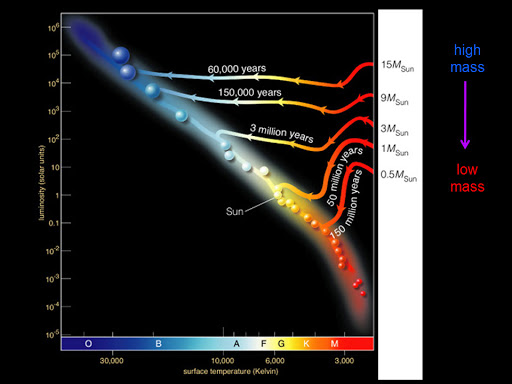
\includegraphics[scale=0.5]{Figures/hayashi_tracks.jpg}
    \caption{Πορείες Hayashi για πρωτοαστέρες διαφόρων μαζών και εγκατάστασή τους στην κύρια ακολουθία.}
    \label{fig:hayashi_tracks}
\end{figure}

Με την πάροδο του χρόνου αυξάνει και η πυκνότητα των εξωτερικών στρωμάτων, με αποτέλεσμα να γίνουν αδιαφανή σε οπτικά μήκη κύματος, ώστε η ακτινοβολία του πυρήνα να μην μπορεί να τα διαπεράσει πλέον. Επομένως, η ακτινοβολούσα επιφάνεια τείνει να συμπέσει με την τελική επιφάνεια του αστέρα. Από τη στιγμή αυτή και μετά, συμβαίνουν δύο βασικά γεγονότα:
\begin{enumerate}
    \item Η συστολή του πρωτοαστέρα συνεχίζεται, αν και με βραδύτερο ρυθμό, και επομένως η επιφάνειά του και η φωτεινότητά του ελλατώνονται (καθοδικό τμήμα της καμπύλης για πρωτοαστέρες με μικρή μάζα στο σχήμα \ref{fig:hayashi_tracks}.
    \item Η θερμοκρασία του πυρήνα αυξάνει σημαντικά, με αποτέλεσμα να αρχίσουν οι πρώτες θερμοπυρηνικές αντιδράσεις.
\end{enumerate}

Κατά τη διάρκεια της καύσης των διάφορων στοιχείων έχουμε ανάσχεση της βαρυτικής συστολής, επειδή η θερμική πίεση του αερίου αντισταθμίζει τη βαρυτική πίεση. Τα ελαφρά στοιχεία D, Li, Be, και B, τα οποία μεταστοιχειώνονται σε χαμηλές θερμοκρασίες, εξαντλούνται γρήγορα επειδή, όπως γνωρίζουμε από μετρήσεις της σχετικής αφθονίας των διάφορων στοιχείων στη φύση, είναι πολύ σπάνια. Όταν η θερμοκρασία φτάσει τους $\sim 10^7 \,\text{K}$, αρχίζει η καύση του άφθονου υδρογόνου σύμφωνα με τη σχέση \eqref{eq:4p_he4} και επιτυγχάνεται θερμική και υδροστατική ισορροπία. Ο αστέρας αρχίζει τη σταδιοδρομία του στην κύρια ακολουθία. Όσο πιο μεγάλη μάζα έχει ένας αστέρας όταν φτάσει στην κύρια ακολουθία, τόσο πιο θερμός και πιο φωτεινός είναι. Επομένως οι αστέρες μεγάλης μάζας εγκαθίστανται στο πάνω αριστερό τμήμα της κύριας ακολουθία, ενώ οι αστέρες μικρής μάζας στο κάτω δεξιό.

Η στιγμή της έναρξης της μεταστοιχείωσης του υδρογόνου στον πυρήνα ενός αστέρα, που συμπίπτει με την εγκατάστασή του στην κύρια ακολουθία, θεωρείται ως η αρχή της ζωής του, αντιστοιχεί δηλαδή σε μηδενική ηλικία. Η πορεία, στο διάγραμμα H-R, που ακολούθησε ο πρωτοαστέρας από τη στιγμή της δημιουργίας του μέχρι να φθάσει στη φάση ενός αστέρα μηδενικής ηλικίας ονομάζεται \textbf{πορεία Hayashi} (Hayashi track). Ο γεωμετρικός τόπος των θέσεων όλων των αστέρων μηδενικής ηλικίας στο διάγραμμα H-R ονομάζεται \textbf{κύρια ακολουθία μηδενικής ηλικίας} (zero age main sequence -- ZAMS). Το χρονικό διάστημα που μεσολαβεί από τη στιγμή της δημιουργίας του πρωτοαστέρα μέχρι τη στιγμή της εγκατάστασής του στην κύρια ακολουθία εξαρτάται από τη μάζα του: είναι μεγάλο για πρωτοαστέρες μικρής μάζας και μικρό για πρωτοαστέρες μεγάλης μάζας. Για τον Ήλιο αυτό το διάστημα υπολογίζεται ότι ήταν $\sim 2 \times 10^7 \,\text{yr}$. Από τα παραπάνω γίνεται σαφής και η διαφορά της ZAMS από την κύρια ακολουθία ενός σμήνους αστέρων: η ZAMS αποτελείται από τις θέσεις των αστέρων \textit{τη στιγμή της δημιουργίας τους}, ενώ η κύρια ακολουθία ενός συνόλου αστέρων (π.χ. ενός σμήνους) αποτελείται από θέσεις αστέρων \textit{διάφορων ηλικιών}, έστω και αν οι αστέρες αυτοί προέρχονται από πρωτοαστέρες που δημιουργήθηκαν ταυτόχρονα, αφού αστέρες διαφόρων μαζών χρειάζονται διαφορετικά χρονικά διαστήματα για να εγκατασταθούν στην κύρια ακολουθία. Επομένως, η ZAMS είναι ένα από πρότυπο χρήσιμο κυρίως για θεωρητικούς υπολογισμούς.
%% ---------------------------------------------------------------------------------------------------- %%
%% ---------------------------------------------------------------------------------------------------- %%
%% ---------------------------------------------------------------------------------------------------- %%
\subsection{Εξέλιξη μετά την κύρια ακολουθία}
Στο μεγαλύτερο μέρος της ζωής τους, οι αστέρες "καίνε" το υδρογόνο τους μετατρέποντάς το σε ήλιο σύμφωνα με τον κύκλο "πρωτονίου-πρωτονίου" (proton-proton chain) ή με τον κύκλο άνθρακα (κύκλος CNO). Όταν ένα σημαντικό ποσοστό του $^1$H μεταστοιχειωθεί σε $^4$He, ο ρυθμός των θερμοπυρηνικών αντιδράσεων ελαττώνεται και γίνεται μικρότερος από το ρυθμό ακτινοβολίας της επιφάνειας του άστρου. Έτσι, υπό την επίδραση της βαρύτητας και μέσω του μηχανισμού Kelvin-Helmholtz, η θερμοκρασία αυξάνεται και ξεκινά  η καύση του $^4$He προς $^{12}$C, με την προϋπόθεση η μάζα του αστέρα να είναι μεγαλύτερη των 0.4 ηλιακών μαζών.

 Η ενέργεια που παράγεται στον πυρήνα εξωθεί τα υπερκείμενα στρώματα με αποτέλεσμα την τεράστια διόγκωση του αστέρα και τη μετατροπή του σε ερυθρό γίγαντα. Αστέρες με μάζα ίση περίπου με την ηλιακή, κατά τη φάση του ερυθρού γίγαντα, χάνουν σε διάστημα 1000 ετών το 20\% με 30\% της μάζας τους σχηματίζοντας τελικά ένα \textit{πλανητικό νεφέλωμα}. Από την φάση του ερυθρού γίγαντα και μετά, ανάλογα με την μάζα ενός αστέρα διαφοροποιείται και η εξέλιξή του. 
%% ---------------------------------------------------------------------------------------------------- %%
%% ---------------------------------------------------------------------------------------------------- %%
%% ---------------------------------------------------------------------------------------------------- %%
\subsubsection{Αστέρες μικρής μάζας}
H συρρίκνωση του αδρανή (αστρικού) πυρήνα $^4$He συνεχίζεται με ταυτόχρονη παραγωγή ενέργειας, μέσω του μηχανισμού Kelvin-Helmholtz, μέχρι τη στιγμή που η αριθμητική πυκνότητα των ηλεκτρονίων σε αυτόν γίνει τόση ώστε αυτά να βρίσκονται σε κατάσταση εκφυλισμού. Για αστέρες με μάζα μικρότερη των $0.8 M_{\odot}$ αυτό συμβαίνει όσο η θερμοκρασία του πυρήνα είναι μικρότερη από τη θερμοκρασία "ανάφλεξης" του $^4$He. Ο αστρικός πυρήνας σταθεροποιείται σε αυτή την κατάσταση και μετατρέπεται σε έναν λευκό νάνο ηλίου. Τα υπόλοιπα στρώματα του αστέρα συνεχίζουν τη διαστολή τους με επιταχυνόμενο ρυθμό,  αντλώντας ενέργεια από την καύση του $^1$H στον φλοιό του αστέρα. Ταυτόχρονα όμως, η βαρυτική έλξη του πυρήνα γίνεται ασθενέστερη καθώς αυτά απομακρύνονται. Σε αυτό το σημείο, ο αστέρας περνά στην φάση του ερυθρού υπεργίγαντα. Κατά τη διάρκεια αυτού του σταδίου, ο αστέρας "σκορπίζεται" στην ευρύτερη περιοχή μέσω του έντονου αστρικού ανέμου που εμφανίζει, δημιουργώντας γύρω του ένα πλανητικό νεφέλωμα. To τελικό αποτέλεσμα είναι ένας λευκός νάνος θερμοκρασίας της τάξης των $30000 \,\text{K}$ που αποτελείται κυρίως από $^4$He και λίγο $^1$H.

%% ---------------------------------------------------------------------------------------------------- %%
%% ---------------------------------------------------------------------------------------------------- %%
%% ---------------------------------------------------------------------------------------------------- %%
\subsubsection{Αστέρες ενδιάμεσης μάζας}
Σε αυτή την κατηγορία έχουμε αστέρες με μάζα που βρίσκεται στο εύρος $0.8 \,M_{\odot} < M < 3 \,M_{\odot}$.
H εξέλιξη αυτών των αστέρων ακολουθεί την πορεία αυτών των μικρότερης μάζας εώς το στάδιο του ερυθρού γίγαντα. Σε αυτή την περίπτωση όμως, η δύναμη της βαρύτητας είναι σημαντικά ισχυρότερη με αποτέλεσμα τα ηλεκτρόνια του αδρανούς πυρήνα $^4$He να εκφυλίζονται και η θερμοκρασία του πυρήνα να ξεπερνά τη θερμοκρασία ανάφλεξης του $^4$He ($2\times 10^{8}K$). Τότε αρχίζει η καυση του $^4$He μέσω της διαδικασίας τριων-α που συζητήσαμε παραπάνω. Όταν όλο το $^4$He που βρίσκεται στον πυρήνα εξαντληθεί έχοντας μετατραπεί σε $^{12}$C και $^{16}$O, ξεκινά η καύση του $^4$He που εντοπίζεται στον εξωτερικό φλοιό του αστρικού πυρήνα, ενώ αυτός περιβάλλεται από έναν φλεγόμενο φλοιό $^1$H ακολουθώντας στο διάγραμμα H-R τον ασυμπτωτικό κλάδο των ερυθρών γιγάντων. Η τελική κατάσταση ενός τέτοιου αστέρα είναι η δημιουργία ενός λευκού νάνου άνθρακα-οξυγόνου.
%% ---------------------------------------------------------------------------------------------------- %%
%% ---------------------------------------------------------------------------------------------------- %%
%% ---------------------------------------------------------------------------------------------------- %%
\subsubsection{Αστέρες μεγάλης μάζας}
Η εξέλιξη αστέρων με μάζα μεγαλύτερη των $3M_{\odot}$ διαφέρει πλέον σημαντικά. Η χαρακτηριστικότερη διαφορά είναι ότι, μετά την εξάντληση των αποθεμάτων άνθρακα και οξυγόνου η θερμοκρασία του πυρήνα είναι πολύ υψηλή και ξεκινάει η μεταστοιχείωσή τους στο επόμενο βαρύτερο στοιχείο, το πυρίτιο (Si). Όσο μεγαλύτερη είναι η μάζα του πυρήνα, οι διαδοχικές μεταστοιχειώσεις προχωρούν μέχρι τη δημιουργία του σιδήρου (Fe). Σε αυτό το σημείο, η διαδικασία διακόπτεται καθώς η περαιτέρω μεταστοιχείωση του σιδήρου είναι μια ενδόθερμη αντίδραση και έτσι η αλυσίδα των συντήξεων σταματά. Σε αυτό το στάδιο, η δομή ενός αστέρα θυμίζει αυτή ενός κρεμμυδιού (onion-like structure) καθώς αποτελείται από πολλά διαφορετικά στρώματα-φλοιούς.
\begin{figure}[h!]
    \centering
    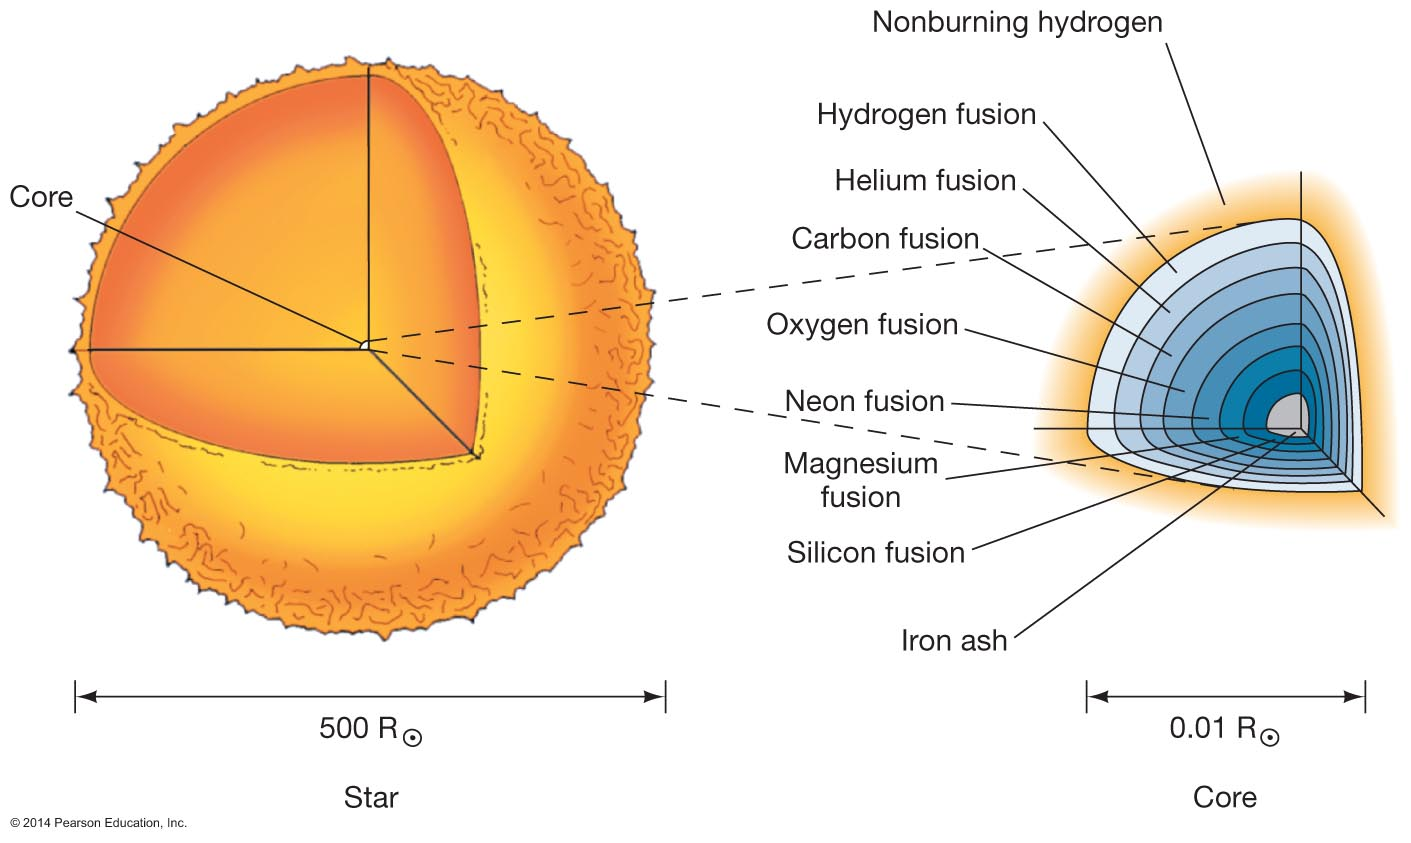
\includegraphics[scale=0.4]{Figures/onion_stellar_structure.jpg}
    \caption{Η δομή "κρεμμυδιού" και η καύση στοιχείων ανά φλοιό κατά τα τελευταία στάδια ζωής ενος αστέρα.}
    \label{fig:onion_stellar_structure}
\end{figure}

Η συνέχεια είναι σε κάθε περίπτωση --κυριολεκτικά-- καταστροφική για τον αστέρα. Με τις σημερινές γνώσεις που έχουμε στην αστροφυσική πιστεύουμε ότι μπορούν να υπάρξουν τέσσερις μόνο τελικές καταστάσεις στις οποίες είναι δυνατόν να καταλήξει ένας αστέρας όταν σταματήσει οριστικά η παραγωγή ενέργειας στον πυρήνα του: 

\begin{itemize}
\item Πλήρης διάλυση του αστέρα
\item Δημιουργία λευκού νάνου
\item Δημιουργία αστέρα νετρονίων
\item Δημιουργία μελανής οπής
\end{itemize}

 Η παραγωγή βαρύτερων στοιχείων του σιδήρου ξεκινά σε κάποιο από τα παραπάνω τελικά στάδια του αστέρα, με διάφορες διεργασίες που μπορούν να λάβουν χώρα και στις οποίες αναφερόμαστε εκτενώς στο παράρτημα \ref{apx:nucleosynthesis}.
%% ---------------------------------------------------------------------------------------------------- %%
%% ---------------------------------------------------------------------------------------------------- %%
%% ---------------------------------------------------------------------------------------------------- %%
\subsubsection{Εξέλιξη στο διάγραμμα H-R}
Η εξέλιξη αστέρων χαμηλής μάζας μπορεί να περιγραφεί ποιοτικά με τη βοήθεια του διαγράμματος H-R ενός σφαιρωτού σμήνους (σχήμα \ref{fig:hrd_evolution}. Παρόλο που το διάγραμμα H-R ενός σμήνους αποτελεί ένα στιγμιότυπο σε μία συγκεκριμένη χρονική στιγμή, παρουσιάζει όλα τα εξελικτικά στάδια στη ζωή ενός αστέρα καθώς η διάρκεια παραμονής ενός αστέρα σε κάθε εξελικτική φάση εξαρτάται από τη μάζα του.

\begin{figure}
    \centering
    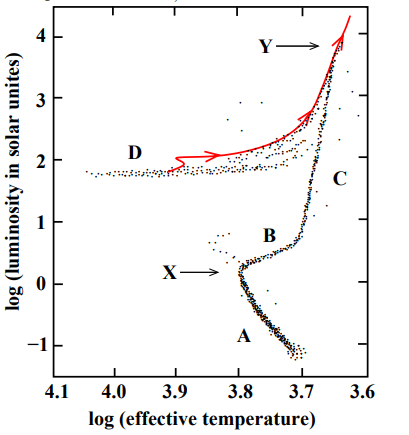
\includegraphics[scale=0.6]{Figures/hrd_evolution.png}
    \caption{Εξέλιξη αστέρων χαμηλής μάζας σε ένα σφαιρωτό σμήνος.}
    \label{fig:hrd_evolution}
\end{figure}

\begin{itemize}
    \item \textbf{Περιοχή A}: Παριστάνει την κύρια ακολουθία. Όλα τα αστέρια σε αυτή την περιοχή είναι στη φάση της κεντρικής καύσης του υδρογόνου, η οποία είναι και η μεγαλύτερη σε χρονική διάρκεια φάση στην ζωή του αστέρα. Αστέρες με χαμηλότερη λαμπρότητα κατά μήκος της κύριας ακολουθίας έχουν χαμηλότερη μάζα καθώς εγκαταστάθηκαν εκεί από διαφορετική πορεία Hayashi.
    \item \textbf{Σημείο στροφής X}: Αστέρες κοντά σε αυτό το σημείο έχουν (σχεδόν) εξαντλήσει το απόθεμα του υδρογόνου στον πυρήνα τους και είναι έτοιμα να αναπτύξουν, πρώτα έναν ισοθερμικό, και έπειτα έναν ηλεκτρονιακά εκφυλισμένο πυρήνα, αφήνωντας πίσω τους την κύρια ακολουθία με το να μετακινηθούν προς χαμηλότερες θερμοκρασίες (δηλαδή την περιοχή B). Παρατηρήστε ότι υπάρχουν μερικά άστρα στην προέκταση της κύριας ακολουθίας, μετά το σημείο στροφής X. Αυτοί οι αστέρες ονομάζονται "κυανοί περιπατητές" (blue stragglers) και είναι ελαφρώς πιο μεγάλοι (σε μάζα) αστέρες που δεν έχουν εξελιχθεί ακόμα πέρα από την κύρια ακολουθία. Αυτά τα αστέρια είναι πιθανόν το αποτέλεσμα των αλληλεπιδράσεων με κάποιο συνοδό αστέρα, ή δημιουργήθηκαν με τη σύγκρουση και συγχώνευση με κάποιο άλλο άστρο στο σφαιρωτό σμήνος (κάτι που συμβαίνει αρκετά συχνά στα πυκνά σφαιρωτά σμήνη).
    \item \textbf{Περιοχές B και C}: Με την έξοδό τους από την κύρια ακολουθία, οι αστέρες γίνονται μεγαλύτεροι (σε διαστάσεις) και πιο λαμπροί και μεταμορφώνονται σε υπογίγαντες (περιοχή B) και τελικά σε γίγαντες (περιοχή C). Στη φάση των γιγάντων, εξελίσσονται με σχεδόν σταθερή ενεργό θερμοκρασία $T_{\text{eff}}$. Σε αυτή τη φάση, οι αστέρες έχουν έναν εκφυλισμένο συμπαγή πυρήνα ο οποίος περιτριγυρίζεται από μία ατμόσφαιρα (convective envelope) που καταλαμβάνει τον μεγαλύτερο όγκο του αστέρα. Η καύση του υδρογόνου συνεχίζεται σε έναν φλοιό που περιβάλλει τον πυρήνα.  
    \item \textbf{Σημείο στροφής Y}: Σε αυτό το σημείο ξεκινάει η καύση του ηλίου στον πυρήνα του αστέρα. Επειδή ο πυρήνας αποτελείται από εκφυλισμένο αέριο ηλεκτρονίων, η ανάφλεξη του ηλίου είναι βίαιη και οδηγεί σε αναπροσαρμογή της δομής του αστέρα (έκλαμψη ηλίου -- helium flash). Παρόλα αυτά, η εκλαμψη δεν είναι αρκετά εκρηκτική για να διαλύσει τον αστέρα. Αντ' αυτού, ο αστέρας επαναπροσαρμόζει τη δομή του και καταλήγει στον οριζόντιο κλάδο του διαγράμματος (περιοχή D). Γι' αυτό, η έκλαμψη ηλίου σηματοδοτεί μία προσωρινή αύξηση στην λαμπρότητα του αστέρα, ορίζοντας την κορυφή του κλάδου των γιγάντων.
    \item \textbf{Περιοχή D}: Αφού επανέλθει σε κατάσταση υδροστατικής και θερμικής ισορροπίας, ο αστέρας περνάει σημαντικό μέρος της ζωής του στον οριζόντιο κλάδο, όπου καίει τα αποθέματα ηλίου στον πυρήνα του, ο οποίος είναι περιτριγυρισμένος από έναν φλοιό στον όποιο πραγματοποιείται καύση υδρογόνου (αυτή είναι συνήθως και η κύρια πηγή ενέργειας). Όταν εξαντληθούν τα αποθέματα του ηλίου στο κέντρο του αστέρα, επιστρέφει στη φάση του ερυθρού γίγαντα με την πορεία που ακολουθεί να προσεγγίζει ασυμπτωτικά τον αρχικό κλάδο των γιγάντων. Σε αυτή την ασυμπτωτική φάση (AGB phase), ο αστέρας έχει έναν εκφυλισμένο πυρήνα που αποτελείται από άνθρακα και οξυγόνο, και περιτριγυρίζεται από έναν φλοιό πλούσιο σε ήλιο και μία πλούσια σε υδρογόνο ατμόσφαιρα. Η πηγή ενέργειας είναι η θερμοπυρηνική σύντηξη του υδρογόνου και του ηλίου που συμβαίνουν σε λεπτούς σφαιρικούς φλοιούς γύρω από τον αδρανή εκφυλισμένο πυρήνα. 
    Επειδή σε αυτό το στάδιο, η ένταση του αστρικού ανέμου είναι πολύ μεγάλη, ο αστέρας χάνει τα εξωτερικά του στρώματα εκθέτοντας τους φλοιούς στους οποίους έχουμε ακόμα καύση. Ο αστέρας έχει πλέον περάσει στη φάση του πλανητικού νεφελώματος στο διάγραμμα H-R και αρζίσει να κινείται προς υψηλότερες θερμοκρασίες με περίπου σταθερή λαμπρότητα. Αυτό συμβαίνει επειδή αρχίζουμε και βλέπουμε πλέον τον πυρήνα του αστέρα που είναι θερμός ενώ η παραγωγή ενέργειας στους φλοιούς παραμένει η ίδια.
    Σε κάποια φάση, η πυρηνική καύση στους φλοιούς θα σταματήσει και ο αστέρας θα αποτινάξει τελείως την ατμόσφαιρά του εκθέτοντας τον πυρήνα του (λευκός νάνος), ο οποίος θα συνεχίσει να ψύχεται εως ότου φτάσει σε θερμική ισορροπία με το υπόλοιπο Σύμπαν.
\end{itemize}
%% ---------------------------------------------------------------------------------------------------- %%
%% ---------------------------------------------------------------------------------------------------- %%
%% ---------------------------------------------------------------------------------------------------- %%